\documentclass[11pt]{article} % Set to 11pt as per the requirements of the teachers
\usepackage{hyperref} % For creating hyperlinks in the table of contents
\usepackage{graphicx}
\usepackage[numbers]{natbib}
\RequirePackage{listings}
\RequirePackage{xcolor}

\usepackage{style/code_style} %Custome style for code highlighting

\linespread{1.38} %The default line spacing for 11pt font size is 1.2, multiplying this by 1.38 gives approximately 1.5 spacing which is required for the report

% Hyperref settings to customize link appearance
\hypersetup{
    colorlinks=true, % Enable colored links
    linkcolor=black, % Color for internal links
    citecolor=green, % Color for citations
    urlcolor=blue % Color for URLs
}

\begin{document}
\begin{titlepage}
    \begin{center}
            
        \Huge
        \textbf{Inventory Management System}
            
        \vspace{0.3cm}
        \Large
        Making Renting and Charching effortless
            
        \vspace{1.0cm}
            
        \textbf{
        Felix Huther,
        Jingya Zhao,
        Kandaker Majharul Islam,
        Philipp Becker,
        Sven Lepper }
          
        \vfill            
        A collaborative project involving\\
        Hochschule Darmstadt (Germany) \\\& Centria University of Applied Sciences (Finnland)

        \vspace{0.5cm}
            
        
\includegraphics[width=0.5\textwidth]{images/logo.png}

            
        \Large
      
        Spring/Summer Term 2024
            
    \end{center}
\end{titlepage}


\tableofcontents
\section{Quote example}
According to \citet{einstein1905}, ...

\section{Content page Ifdi}


\section{Introduction}
{\tiny Written by: Philipp Becker}\\
\subsection{Main Vision}
This Inventory Management System simplifies the process of renting out lockers within educational institutions. Users can easily search for and rent lockers to charge their devices, as well as essential items such as laptops and chargers. Meanwhile, administrators benefit from device tracking, and comprehensive reporting tools. All of these contribute to increased efficiency and convenience for all stakeholders.

Option:
Our Inventory Management System revolutionizes the way educational institutions manage and rent lockers, promoting efficiency, inclusivity, and sustainability. Users can effortlessly search for and rent lockers to charge their devices or store essential items like laptops and chargers. This system not only simplifies the process for users but also provides administrators with advanced device tracking and comprehensive reporting tools. These features collectively contribute to a seamless, stress-free experience, enhancing productivity and convenience for all stakeholders.

\subsection{Core Values and Project Goals}
Core values are fundamental principles and beliefs that guide the behavior and decision-making process within an organization. They represent the essence of what the organization stands for and help shape its culture and identity. Our chosen core values are Sustainability, Equality, and Stress-less. We selected these values because they align with our vision of creating a responsible, inclusive, and user-friendly Inventory Management System.

\begin{enumerate}
\item Sustainability: We aim to incorporate eco-friendly practices in our system, such as promoting the use of energy-efficient devices and reducing waste. Our goal is to ensure that our operations have a positive impact on the environment, contributing to a healthier planet and setting a positive example for others.
\item Equality: We are committed to providing equal access and opportunities for all users, regardless of their background or circumstances. This involves ensuring our system is accessible to everyone, offering fair rental terms, and fostering an inclusive environment. Our goal is to support equal education by making essential tools and resources available to all students.

\item Stress-less: Our objective is to create a user-friendly system that minimizes the stress associated with managing and renting equipment. By streamlining processes, offering intuitive interfaces, and providing timely maintenance reminders, we make it easier for both users and administrators to interact with our system. A stress-free experience enhances satisfaction and productivity for all parties involved.
\end{enumerate}

By adhering to these core values, our project goals focus on achieving a sustainable, equitable, and user-friendly system that meets the needs of all stakeholders.

\subsection{Core Functionalitys}
\subsubsection{Renting Devices and Lockers}
\begin{itemize}
\item \textbf{Renting Devices:} Users can rent devices through an intuitive interface, which allows them to select, reserve, and access devices based on availability and specific needs. The devices available for rent are stored in lockers and can be picked up using a provided access code.
\item \textbf{Renting Lockers:}  The system provides capabilities for users to rent lockers, facilitating a secure and convenient way to store personal devices within the facility. Additionally, users can charge their devices in the rented locker and monitor the wattage flow through the frontend interface.
\end{itemize}

\subsubsection{Managing Devices \& Lockers}
\begin{itemize}
\item \textbf{Manage Devices:} Administrators can create, categorize, and manage devices. They have the ability to oversee all device allocations, track device status, update device information, and view all bookings.

\item \textbf{Manage Lockers:} This feature allows administrators to create and manage lockers and monitor their status. Administrators can also view and manage all locker bookings.
\end{itemize}

\subsubsection{Reporting and Manage Problems}
\begin{itemize}

\item \textbf{Report Problems: }Users can report any issues they encounter with the devices or lockers, such as malfunctions or access problems. The problems, along with all relevant booking information, are sent to the administrator.

\item \textbf{Manage Problems: }Enables the administration to efficiently handle and resolve reported problems related to devices or lockers, improving service quality and user satisfaction.
\end{itemize}


\subsection{Team Composition and Responsibilities}
In this project, members were divided into specific teams based on their interests and expertise. Each team was assigned specific components of the project, ensuring that their distinct expertise contributed to the comprehensive development and integration of the system, while also collaborating effectively to meet the project's overarching goals. This section outlines the team structure, member assignments, and their respective responsibilities. 
\newpage
\subsection{Team Introduction}
\subsubsection{Jingya Zhao}
Centria University of Applied Sciences \\
Degree Program: Information Technology
\begin{figure}[h]
    \centering
    
\includegraphics[width=0.2\textwidth]{images/jingya.JPG}
\end{figure}

\subsubsection{Kandaker Majharul Islam}
Centria University of Applied Sciences \\
Degree Program: Information Technology
\begin{figure}[h]
    \centering
    
\includegraphics[width=0.2\textwidth]{images/ifty.JPG}
\end{figure}

\subsubsection{Felix Huther}
Hochschule Darmstadt, University of Applied Sciences \\
Degree Program: Computer Science
\begin{figure}[h]
    \centering
    
\includegraphics[width=0.2\textwidth]{images/felix.JPG}
\end{figure}

\subsubsection{Sven Lepper}
Hochschule Darmstadt, University of Applied Sciences \\
Degree Program: Computer Science
\begin{figure}[h]
    \centering
    
\includegraphics[width=0.2\textwidth]{images/sven.JPG}
\end{figure}

\subsubsection{Philipp Becker}
Hochschule Darmstadt, University of Applied Sciences \\
Degree Program: Computer Science
\begin{figure}[h]
    \centering
    
\includegraphics[width=0.2\textwidth]{images/philipp.JPG}
\end{figure}
\newpage
\subsection{Workload Definition}

Each team in our project defined their own set of work packages using ClickUp, a versatile tool designed to manage task-based work through a Kanban board visualization. Afterward, we collaboratively addressed cross-team responsibilities and integration tasks. Every three days, we discussed these tasks together, ensuring continuous alignment with project goals and effective problem-solving.

info: better ?

\begin{figure}[h]
    \centering
    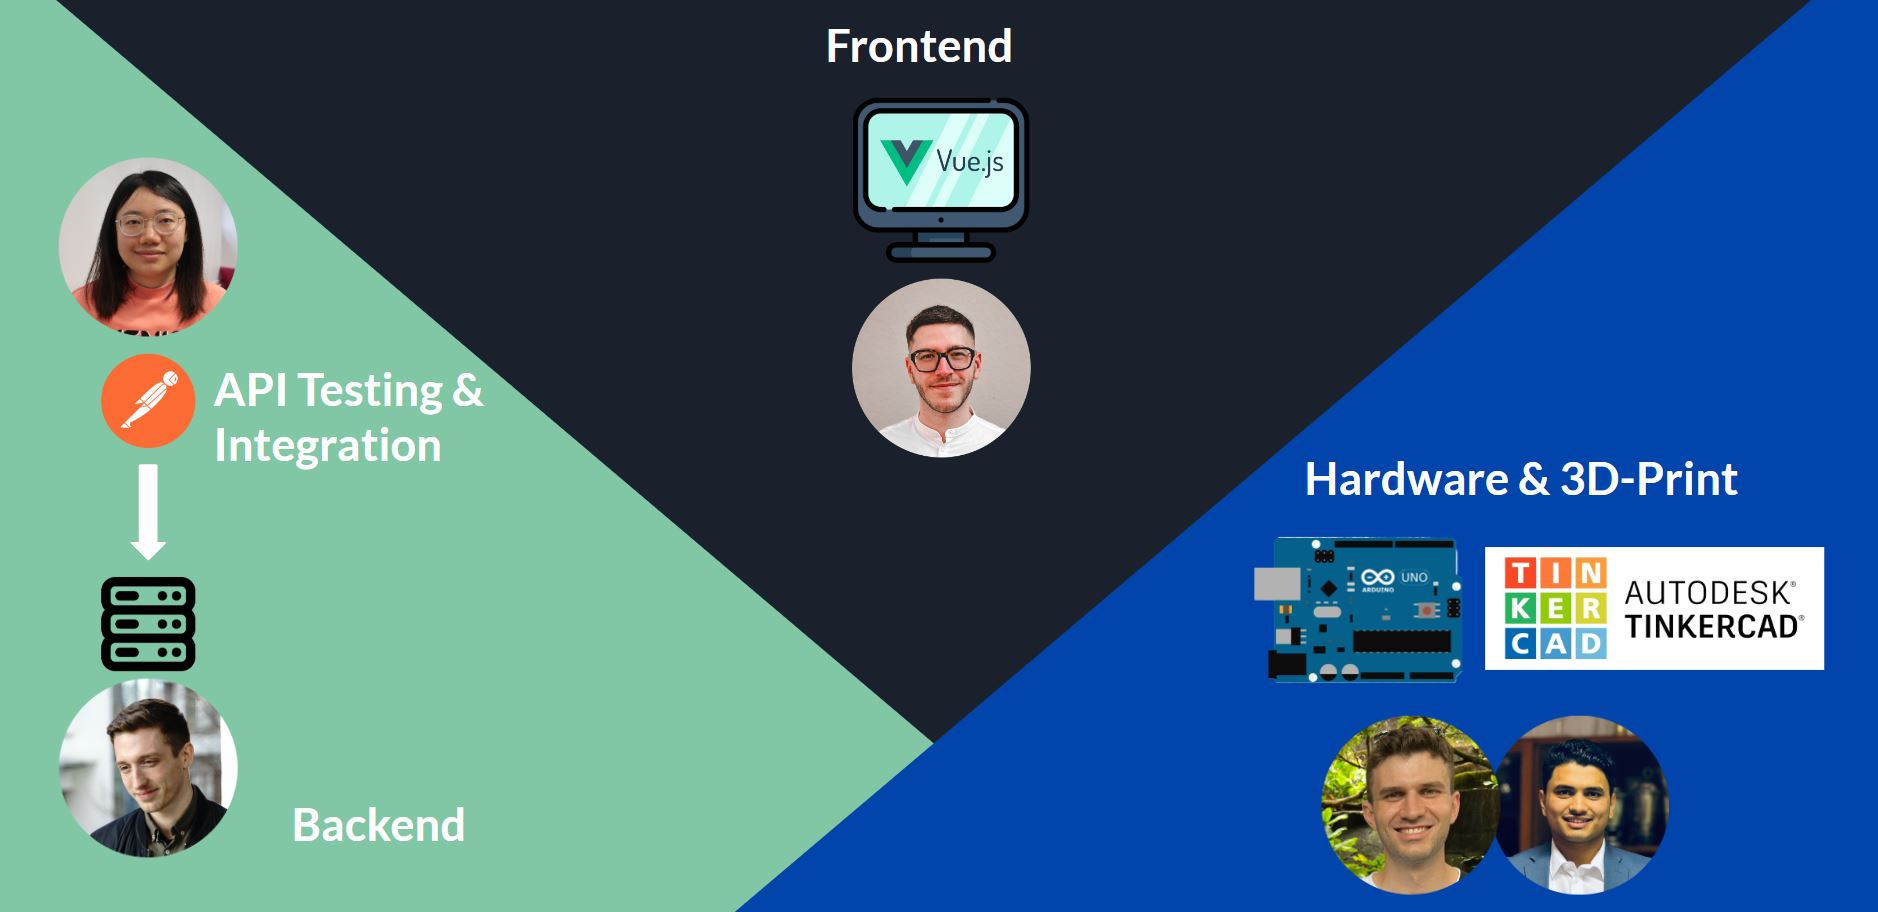
\includegraphics[width=0.8\textwidth]{images/workload.JPG}
    \caption{Team Composition and Responsibilities}
\end{figure}


%Each team in our project independently defined their own set of work packages using ClickUp, a versatile tool designed to manage task-based work through a Kanban board visualization. This approach allowed every team member to clearly see their tasks and responsibilities, facilitating better planning and coordination. To maintain momentum and ensure continuous alignment with project goals, the teams reviewed the board every three days. These meetings served as mini-sprints, akin to the Scrum methodology, where progress was assessed, and adjustments were made as necessary.

\clearpage
\subsubsection{Hardware and 3D Print}
The Hardware and 3D Printing team was led by Felix Huther, with significant assistance from Kandaker Majharul Islam. Felix was primarily responsible for designing the 3D models, overseeing the prototype printing, and managing the hardware assembly. Kandaker supported Felix in all these tasks and was introduced to programming the Arduino device, where he implemented several smaller functions. This team also integrated REST APIs for real-time data transmission, sending live data to the frontend via ThingSpeak and ensuring backend communication.

\begin{figure}[htbp]
    \centering
    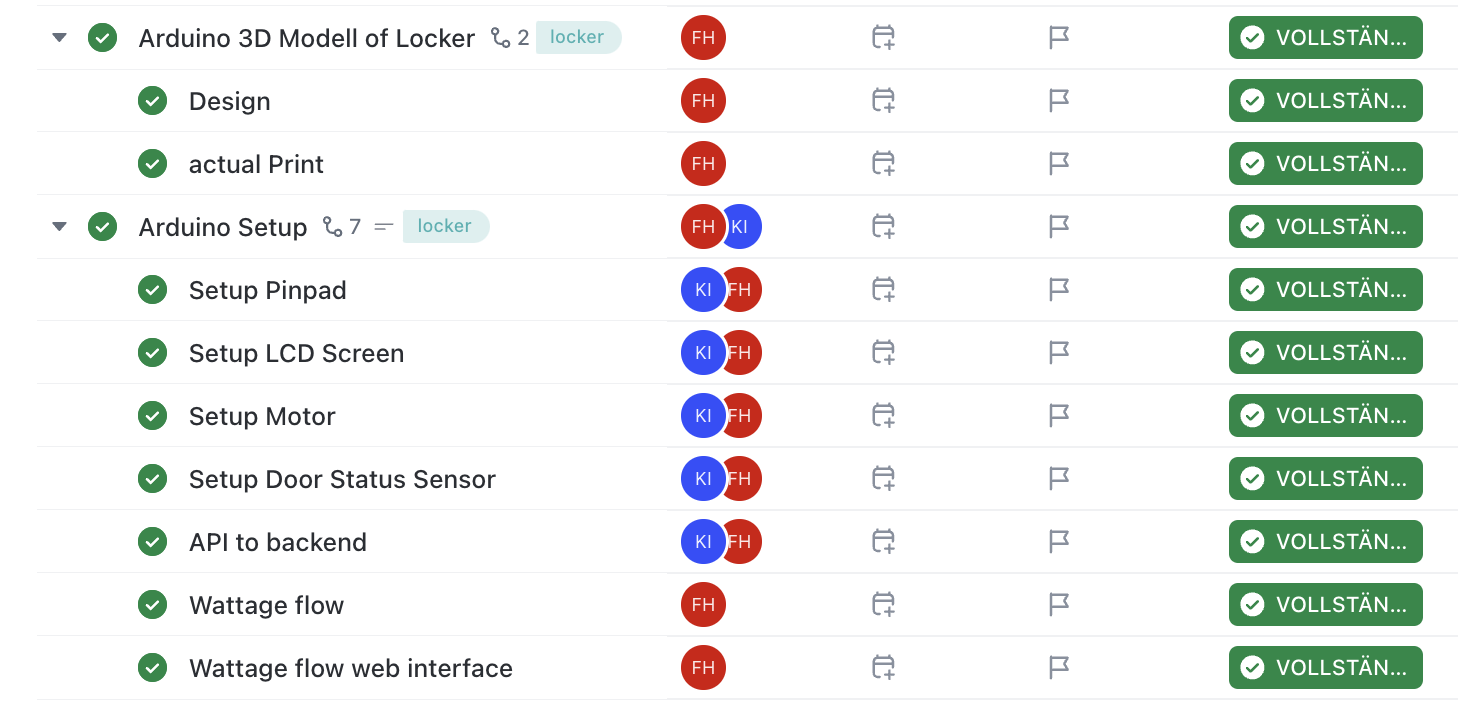
\includegraphics[width=0.9\textwidth]{images/hardware and print.png}
    \caption{Hardware and 3D Model Tasks}
    \label{fig:myimage}
\end{figure}

\subsubsection{Frontend Development}
Philipp Becker was responsible for the Frontend development, utilizing Vue.js in TypeScript, styled with Tailwind CSS and Vue-Bootstrap. This setup facilitated a robust and responsive user interface. Philipp also integrated the Google Maps API to show the current location of the locker on a map. The frontend implementation was split into two tasks: Admin-Frontend for administrative tasks such as management, reports, and bookings, and User-Frontend for locker rentals, device rentals, and problem reporting.


\begin{figure}[htbp]
    \centering
    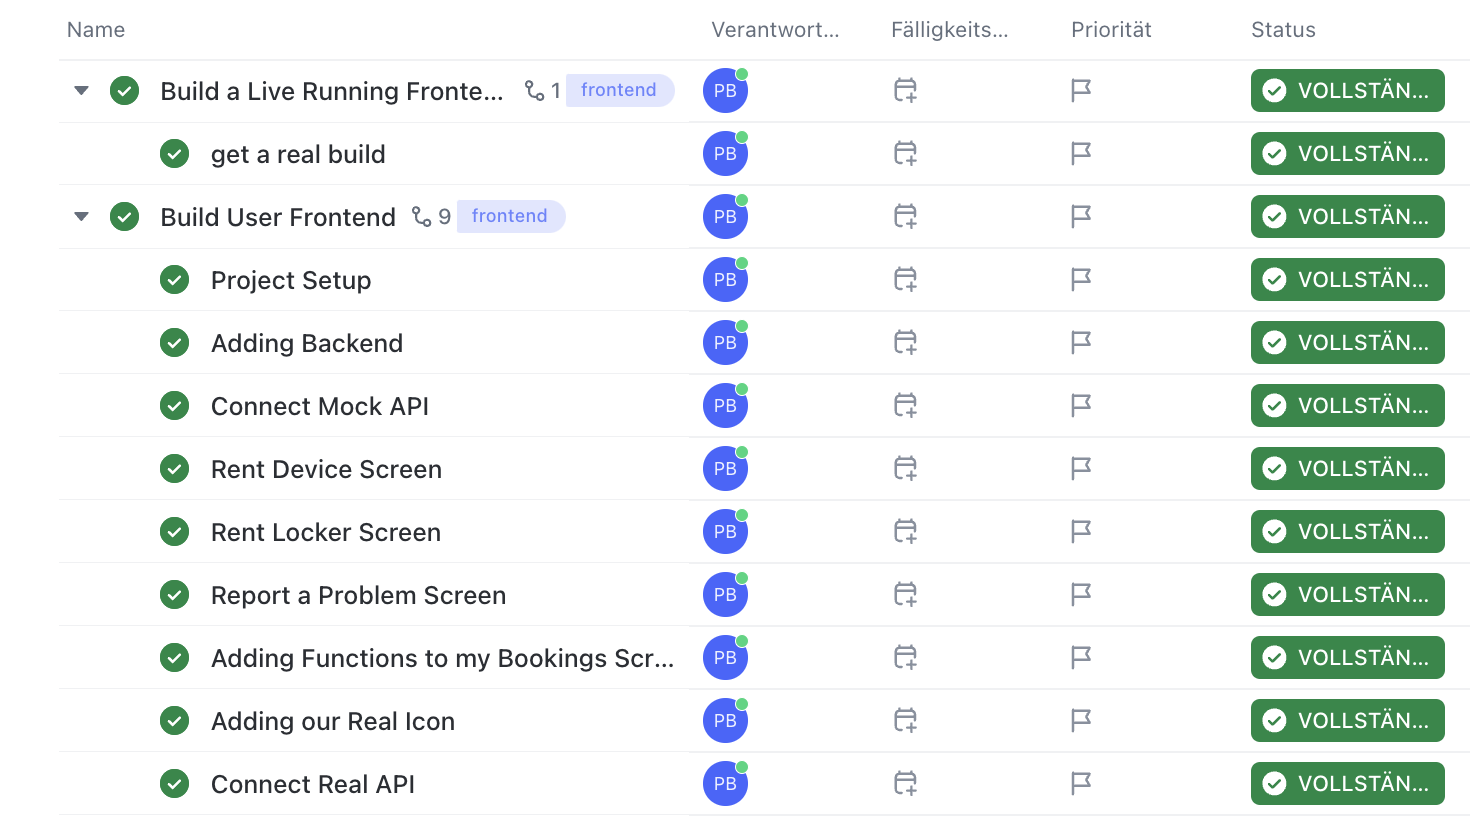
\includegraphics[width=0.9\textwidth]{images/user-frontend.png}
    \caption{User-Frontend Tasks}
    \label{fig:myimage}
    \vspace{1cm}
    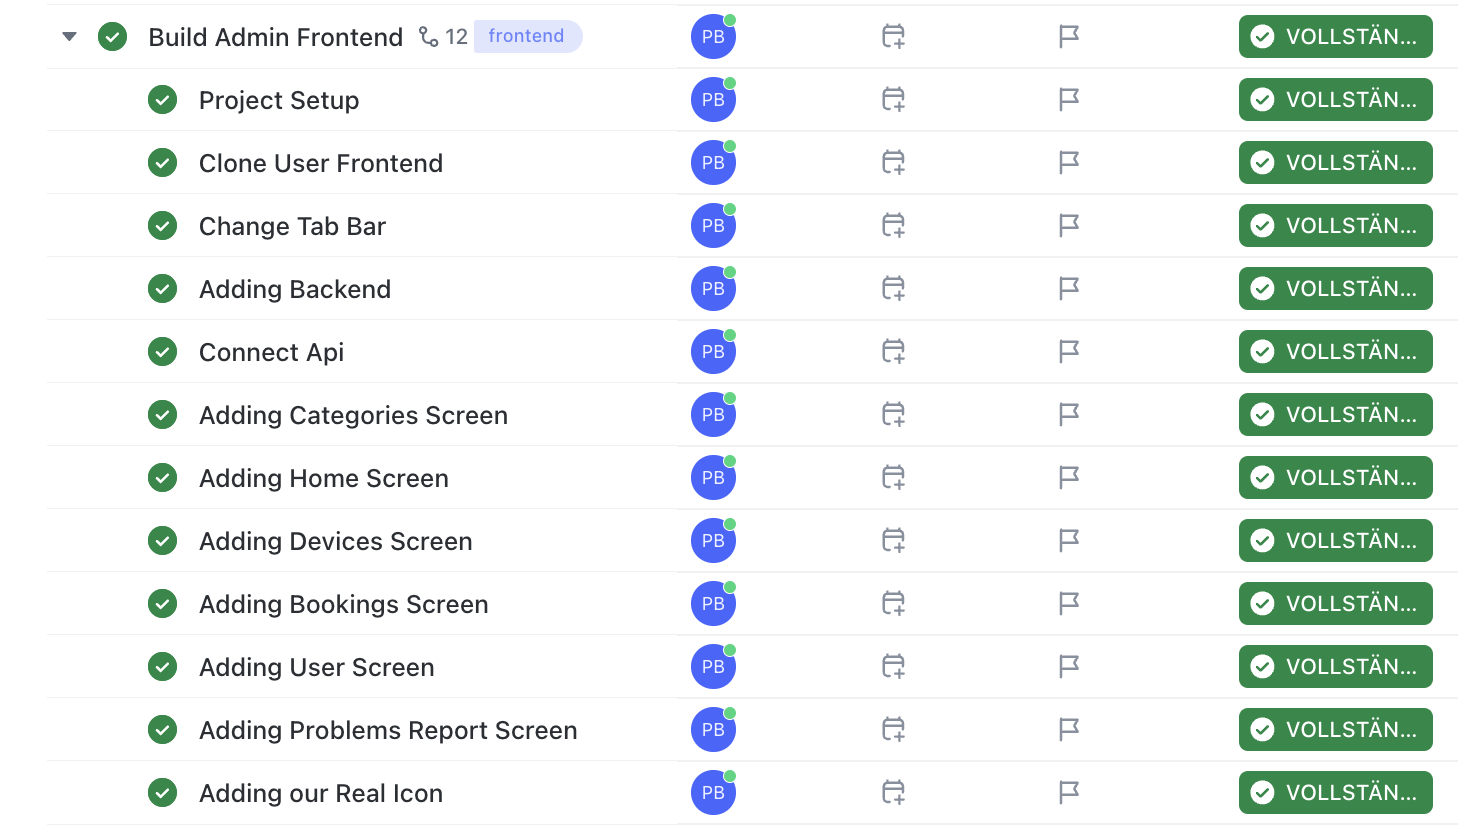
\includegraphics[width=0.8\textwidth]{images/admin-frontend.png}
    \caption{Admin-Frontend Tasks}
    \label{fig:myimage}
\end{figure}
\clearpage
\subsubsection{Backend Development}
Sven Lepper handled Backend development, employing Alembic with SQL Alchemy as the Object-Relational Mapper (ORM) and PostgreSQL for database management. Fast API was used to create a RESTful interface, enabling efficient communication between all components and the database. This setup provided a solid backbone for the application's data handling requirements.

\begin{figure}[h]
    \centering
    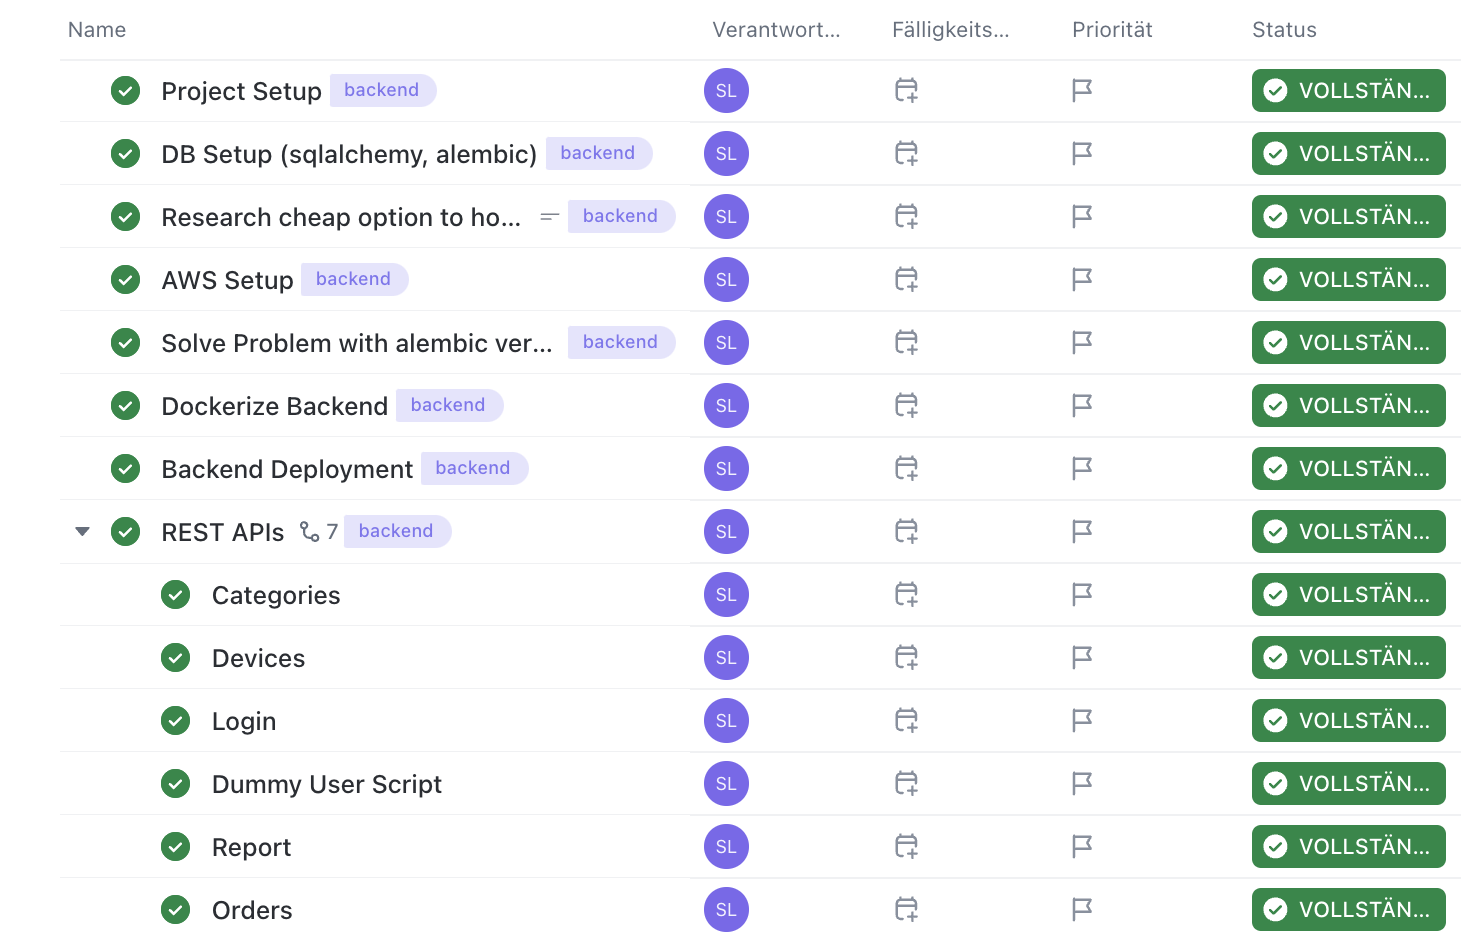
\includegraphics[width=0.9\textwidth]{images/backend.png}
    \caption{User-Frontend Tasks}
    \label{fig:myimage}
\end{figure}
\clearpage
\subsubsection{API Testing and Hardware Research}
Jingya Zhao took charge of API Testing and Hardware Research. She developed automated tests using Postman, which validated the correctness of data across all backend endpoints. Additionally, Jingya conducted research on live tracking technologies for monitoring the energy usage of devices, which was crucial for the real-time data feature in the project.

\begin{figure}[h]
    \centering
    
\includegraphics[width=0.9\textwidth]{images/R&d.png}
    \caption{Hardware Research Tasks}
    \label{fig:myimage}
    \vspace{1cm}
    
\includegraphics[width=0.9\textwidth]{images/testing.png}
    \caption{API Testing Tasks}
    \label{fig:myimage}
\end{figure}


\section{Motivation}
{\tiny Written by: Jingya Zhao}\\

This project was inspired by a presentation on a equipment database, which addressed functionalities for adding equipment data, searching the database, and managing equipment borrowing and returns. The presentation highlighted the importance of some features:
\begin{itemize}
    \item Tracking equipment details (owner, purchase date, location)
    \item Searching equipment by type, brand, and location
    \item Reserving equipment
    \item Reporting equipment issues
\end{itemize}

These functionalities match perfectly with the challenges faced by universities in managing tech equipment. Universities typically rely on manual processes, leading to limited access for students, difficulties managing device charging, and a burden on IT staff for equipment tracking and maintenance.

We saw an opportunity to utilise the principles underlying equipment databases. This led us to develop a locker system that could address these limitations. The locker system would provide:
\begin{itemize}
    \item Easy access for students: Allowing them to reserve and pick up equipment through a user-friendly interface.
    \item Uninterrupted use for professors: Offering dedicated lockers for charging personal devices.
    \item Efficient management for IT administrators: Providing an automated system for booking and device tracking, eliminating manual processes.
\end{itemize}

To ensure a smooth experience for all users, we decided to design four key functions for the locker system:

\begin{enumerate}
    \item \textbf{Device Rental}: Users can browse and reserve equipment through a user-friendly website. Once reserved, a unique code is provided for locker access. This same code allows them to retrieve the equipment and return it. Users can easily report any broken or malfunctioning equipment directly through the website.
    \item \textbf{Device Charging}: Lockers can be used to conveniently charge personal devices. The system displays real-time power consumption information, allowing users to monitor their device's charging status.
    \item \textbf{IT Admin Management}: IT administrators can efficiently manage all devices and bookings within the system. This includes adding new equipment, tracking reservations, and overseeing overall system operations.
    \item \textbf{Equipment Issue Reporting}: Users can easily report any broken or malfunctioning equipment directly through the website. This ensures prompt maintenance and helps maintain the quality and availability of the equipment.
\end{enumerate}

By creating this university locker system, we aimed to improve accessibility, convenience, and overall equipment management for the university community.

\section{Methodology}
{\tiny Written by: Felix}\\

\begin{enumerate}
    \item which are the steps that are taken 
    in which order to reach the result
    \item which steps are taken
    \item which tools were used (keep this short)
    \item always give reasons for WHY you chose 
    certain steps
    \item always give reasons for WHY you 
    chose certain tools
\end{enumerate}

In this section, we outline the methodology used for the project, covering planning, design, development, integration, and deployment phases.

\subsection{Planning Phase}

Effective planning is crucial for the success of our project, especially considering our unique work arrangement. With only one week of in-person collaboration and the majority of our work conducted online, meticulous planning becomes essential to ensure smooth coordination, clear communication, and efficient task management. This phase lays the groundwork for our project's success by defining roles, establishing communication channels, and outlining our approach to project execution. By emphasizing thorough planning, we aim to maximize productivity, maintain team cohesion, and overcome the challenges posed by our distributed work environment.

\begin{enumerate}
    \item \textbf{Team Building}:
    \begin{itemize}
        \item Formed a collaborative and diverse team through spontaneous selection based on available participants. The team consisted of individuals from various international backgrounds, including Finnish \& German students and other participants, fostering a multicultural and multidisciplinary environment.
        \item Leveraged the diverse composition of the team to promote cross-cultural perspectives and interdisciplinary collaboration, enhancing creativity and problem-solving capabilities during project execution.
    \end{itemize}
    
    \item \textbf{Project Selection}:
    \begin{itemize}
        \item Engaged in a facilitated process where a professor from Centria University presented a range of project topics to the team. Each topic was evaluated based on criteria such as feasibility, innovation potential, and alignment with organizational goals.
        \item Collaboratively deliberated and selected the most promising project topic from the options provided, considering the team's capabilities and interests.
    \end{itemize}
    \textbf{Why we decided for project}
    \begin{enumerate}
        \item The team expressed a strong interest and enthusiasm for topics related to databases, frontend development, and locker systems, reflecting our collective passion and desire to deepen our expertise in these areas.
        \item Recognizing the importance of specialization and professional growth, we chose these topics to leverage our existing skills and gain hands-on experience in critical aspects of modern software development.
        \item By focusing on database management, frontend design, and locker system implementation, we aimed to enhance our proficiency and readiness to tackle real-world challenges in these specialized domains.
        \item Our commitment to professionalism motivated us to select topics that align with our career aspirations and provide valuable learning opportunities to develop industry-relevant skills.
        \item Additionally, we identified strong future perspectives and potential career opportunities associated with database management, frontend development, and smart locker systems, making these topics strategic choices for our educational and professional growth.
    \end{enumerate}
    

    \item \textbf{Project Brainstorm}:
    \begin{itemize}
        \item Conducted facilitated brainstorming sessions to generate creative ideas and identify key project features and requirements based on stakeholder inputs.
        \item \textbf{Why we conducted brainstorming sessions}:
            \begin{enumerate}
                \item Emphasized inclusivity and openness to ensure all team members could freely contribute their ideas without constraints.
                \item Focused on capturing a wide range of ideas and perspectives to explore innovative solutions and address diverse project requirements.
                \item Encouraged collaborative idea generation to foster team cohesion and collective ownership of project concepts.
                \item Recognized the importance of comprehensive planning and idea exploration to minimize the risk of overlooking critical aspects of the project.
            \end{enumerate}
    \end{itemize}



    \item \textbf{Organizational Structure}:
    \begin{itemize}
        \item Defined clear roles and responsibilities within the team and established communication channels to ensure effective collaboration and coordination throughout the project lifecycle.
        \item \textbf{Why we defined the organizational structure}:
            \begin{enumerate}
                \item Facilitated clear understanding of individual roles and responsibilities, promoting accountability and ownership within the team.
                \item Established efficient communication channels and workflows to facilitate seamless collaboration and coordination among team members.
                \item Enhanced project management and coordination by assigning specific tasks and defining decision-making processes.
                \item Ensured smooth project execution by clarifying who organizes meetings, manages tasks, and facilitates team interactions.
            \end{enumerate}
            \item \textbf{Communication Tools Used}:
            \begin{enumerate}
                \item \textbf{ClickUp (Kanban Board)}: Implemented ClickUp as a Kanban board tool to manage tasks, track progress, and visualize workflow stages, enabling efficient project planning and task management.
                \item \textbf{GitHub}: Utilized GitHub for version control and collaboration on project repositories, allowing team members to share and synchronize code, track changes, and manage project documentation.
                \item \textbf{Discord}: Utilized Discord as a primary platform for organizing project discussions, sharing updates, and facilitating real-time communication among team members.
                \item \textbf{WhatsApp}: Leveraged WhatsApp for conducting polls, scheduling meetings, and exchanging short messages for quick updates and coordination.
                \item \textbf{Google Calendar}: Used Google Calendar as a centralized platform for scheduling meetings and appointments, ensuring consistency across different time zones and facilitating team coordination.
                \item \textbf{Google Drive}: Utilized Google Drive for organizing presentations, documents, and images, providing a collaborative workspace for sharing and accessing project-related resources.
            \end{enumerate}        
    \end{itemize}
\end{enumerate}


\subsection{Design Phase}

\begin{enumerate}
    \item \textbf{Personas}:
    \begin{itemize}
        \item Developed user personas based on target audience demographics, behaviors, and needs to guide design decisions and prioritize features.
        \item \textbf{Why we developed user personas}:
            \begin{enumerate}
                \item Gained insights into the preferences, behaviors, and needs of our target audience to inform design decisions and feature prioritization.
                \item Enabled a user-centered design approach by creating fictional representations of potential users, ensuring that our solutions address real-world user requirements.
                \item Facilitated empathy and understanding among team members by visualizing and empathizing with user personas, enhancing our ability to design intuitive and user-friendly interfaces.
                \item Supported stakeholder engagement and decision-making processes by aligning design choices with identified user preferences and challenges.
            \end{enumerate}
    \end{itemize}

    
    \item \textbf{Use Cases}:
    \begin{itemize}
        \item Defined use cases to capture interactions between users and the system, facilitating a clear understanding of functional requirements and user workflows.
        \item \textbf{Why we defined use cases}:
            \begin{enumerate}
                \item Enhanced clarity and specificity in defining system functionalities and user interactions, ensuring alignment with project objectives.
                \item Enabled systematic validation of system behavior against user requirements, identifying potential mistakes and gaps in functionality.
                \item Provided a clear and structured representation of user workflows, guiding the design and development process to meet user expectations.
                \item Supported effective communication among team members and stakeholders by visualizing user-system interactions and functional requirements.
            \end{enumerate}
    \end{itemize}

    \item \textbf{Wireframes}:
    \begin{itemize}
        \item Created wireframes using \textbf{Miro} to visualize the user interface layout and navigation structure, allowing for early feedback and iteration on design concepts.
        \item \textbf{Why we created wireframes}:
            \begin{enumerate}
                \item Facilitated the rapid prototyping of frontend design concepts, enabling quick visualization and validation of UI layout and navigation.
                \item Provided a tangible representation of the user interface, allowing for early feedback and iteration to refine design concepts and improve usability.
                \item Supported user testing activities by presenting a preliminary version of the UI, enabling stakeholders and end-users to provide valuable feedback.
                \item Enhanced collaboration among team members and stakeholders by aligning design expectations and ensuring a shared vision of the final product.
            \end{enumerate}
    \end{itemize}
    
    \item \textbf{Wireframe Tool Used}:
        \begin{itemize}
            \item \textbf{Miro (Wireframing)}: Employed Miro for wireframing due to its ease of use and ability to deliver fast results. Miro's online platform facilitated seamless sharing and collaboration among team members, enhancing creativity and enabling remote collaboration on design concepts and workflows.
        \end{itemize}


    \item \textbf{Software Architecture}:
    \begin{itemize}
            \item Designed a scalable and modular software architecture to support future expansion and maintenance of the system.       
    \item \textbf{Architecture Tools Used}:
        \begin{enumerate}
            \item \textbf{Frontend: Tailwind CSS and Vue.js}: Employed Tailwind CSS and Vue.js for frontend development. Tailwind CSS offers utility-first styling, facilitating rapid UI development, while Vue.js provides a reactive framework for building interactive user interfaces.
            \item \textbf{Backend: FASTAPI, SQLAlchemy, Docker}: Implemented the backend using FASTAPI for creating RESTful APIs, SQLAlchemy for database interaction, and Docker for containerization. FASTAPI's asynchronous capabilities and SQLAlchemy's ORM simplifies backend development, while Docker ensures easy deployment and scalability.
            \item \textbf{Hardware Sensors (Refer to Section \ref{sec:ArduinoSensors})}: Utilized various sensors as detailed in Section 7.5.4 for hardware integration within the system, enabling data collection and interaction with physical components.
        \end{enumerate}
    \end{itemize}
    
    
    \item \textbf{3D Modeling}:
    \begin{itemize}
            \item Created 3D models using \textbf{Tinkercad} to visualize physical components and interactions within the system, aiding in the development of prototypes and simulations.
        \item \textbf{3D Modeling Tools Used}:
        \begin{enumerate}
            \item \textbf{Tinkercad \cite{tinkercad}}: Selected Tinkercad as our 3D modeling tool for its intuitive interface and online accessibility, making it ideal for team members new to 3D modeling. The tool's manageable learning curve allowed quick understanding of 3D modeling concepts, facilitating efficient creation of prototypes and simulations. Additionally, Tinkercad's online platform promoted seamless collaboration and sharing of 3D models among team members, enhancing teamwork and productivity.
        \end{enumerate}
    \end{itemize}
\end{enumerate}
   

\subsection{Development Phase}

\begin{enumerate}

    \item \textbf{Implementation}:
    \begin{itemize}
        \item Implemented core features and functionalities based on design specifications, utilizing appropriate programming languages and frameworks.
        \item \textbf{Technologies Used}:
            \begin{enumerate}
                \item \textbf{Frontend (Vue.js)}: Started frontend implementation using Vue.js, a progressive JavaScript framework for building user interfaces. Vue.js was chosen for its simplicity, reactivity, and component-based architecture, allowing rapid development of interactive frontend components.
                \item \textbf{Backend (Python with FASTAPI)}: Developed the backend using Python with FASTAPI, a modern web framework for building APIs with asynchronous support. FASTAPI's performance and ease of use were instrumental in creating scalable backend services.
                \item \textbf{Database (PostgreSQL with SQLAlchemy)}: Integrated PostgreSQL as the database management system, leveraging SQLAlchemy as the ORM (Object-Relational Mapping) tool. PostgreSQL was chosen for its reliability, SQL compliance, and seamless integration with SQLAlchemy, simplifying data modeling and interaction within the application.
                \item \textbf{Hardware (Arduino)}: Arduino emerged as the ideal choice for our project due to its ease of use for our team and the availability of compatible hardware components. This facilitated efficient prototyping and sensor integration.
            \end{enumerate}
    \end{itemize}


    \item \textbf{Bi-weekly Meetings}:
    \begin{itemize}
        \item Conducted regular bi-weekly meetings, modeled after stand-up meetings, to review project progress, address challenges, and align project goals with stakeholders.
        \item \textbf{Meeting Format}:
            \begin{enumerate}
                \item Team members provided updates based on Kanban board tasks:
                    \begin{itemize}
                        \item What they accomplished since the last meeting.
                        \item Current tasks they are working on.
                        \item Planned tasks for the upcoming period.
                        \item Challenges or blockers they are facing.
                    \end{itemize}
                \item Encouraged problem-solving discussions to address challenges collaboratively within the team.
            \end{enumerate}
        \item \textbf{Communication Tools Used}:
            \begin{enumerate}
                \item \textbf{Google Meet or Discord}: Leveraged Google Meet or Discord as the primary platforms for conducting bi-weekly meetings. These tools facilitated real-time communication, screen sharing, and video conferencing, enabling effective discussions and updates among team members located remotely.
            \end{enumerate}
    \end{itemize}


 \item \textbf{Research and Development (R\&D)}:
    \begin{itemize}
        \item Invested time in R\&D to explore innovative solutions and technologies that could enhance project outcomes and performance.
        \item \textbf{R\&D Initiatives}:
            \begin{enumerate}
                \item Explored methods for displaying device battery status, ultimately opting for an intermediate solution that indicates power flow through the cable. This approach addressed immediate needs while paving the way for more sophisticated battery monitoring solutions in the future.
                \item Conducted research on deploying frontend and backend components, leveraging Google as a key tool for accessing documentation, tutorials, and best practices. Google facilitated the acquisition of valuable insights and guidance, aiding in the successful deployment of project components.
            \end{enumerate}
    \end{itemize}

    
\item \textbf{Building Prototype}:
    \begin{itemize}
        \item Developed functional prototypes to validate design assumptions that we can start installing the sensors with the Deployment Phase.
    
    \item \textbf{3D Printing Tool}:
    \begin{enumerate}
        \item Used the Anycubic Kobra 3D \citet{anycubic-kobra} printer to manufacture prototypes, enabling the installation of various sensors and components to support design validation and iterative development.
    \end{enumerate}
    \end{itemize}
\end{enumerate}



\subsection{Integration Phase}

\begin{enumerate}
    \item \textbf{Component Integration}:
    \begin{itemize}
        \item Integrated individual components and subsystems to ensure seamless interoperability and overall system functionality. Testing included using Postman for FastAPI, manual testing for Arduino components, and ESLint for frontend code analysis.
    \end{itemize}

\item \textbf{Usability Test}:
    \begin{itemize}
        \item Conducted usability testing sessions on the frontend to evaluate design and usability aspects. Results from these tests informed UX improvements for enhanced user experience.
    \end{itemize}

\item \textbf{Integration Test}:
    \begin{itemize}
        \item Performed integration testing to validate end-to-end system functionality and identify compatibility issues. Leveraged automated tests with Postman for API interactions to ensure components work together seamlessly.
    \end{itemize}

\end{enumerate}



\subsection{Deployment Phase}

\begin{enumerate}
    \item \textbf{Frontend Deployment}:
        \begin{itemize}
            \item Deployed frontend components of the system to web servers or cloud platforms to make the user interface accessible to end-users. We chose Netlify for frontend deployment due to its simplicity and seamless integration with Git, enabling continuous deployment and easy updates of the user interface.
        \end{itemize}
        Detailed information on the frontend deployment with Netlify can be found in Section \ref{sec:Frontend_Implementation} 

    \item \textbf{Backend Deployment}:
        \begin{itemize}
            \item Deployed backend services and APIs to support the application logic and data processing tasks. The backend, including the database system, was deployed using Google Cloud Run solutions. Google Cloud Run's serverless architecture allowed for scalable and efficient deployment of backend components without managing infrastructure overhead.
        \end{itemize}
        Detailed information on the backend deployment with Google Cloud Run can be found in Section \ref{sec:Implementation_Backend}
\end{enumerate}

This methodology provided a structured approach to project planning, design, development, integration, and deployment, ensuring efficient execution and successful delivery of the project objectives.

\section{Software Design}
{\tiny Written by: Sven}

\subsection{Introduction}

This chapter delves into the intricate details of the software design employed in the
development of the locker system for university environments. A robust and efficient
software architecture is pivotal in ensuring the seamless functioning and user satisfaction
of the system. In this section, we provide an overview of the architectural approach,
technologies, and frameworks chosen for the implementation of the locker system software,
highlighting their significance and relevance to the project objectives.

\begin{figure}[h]
    \centering
    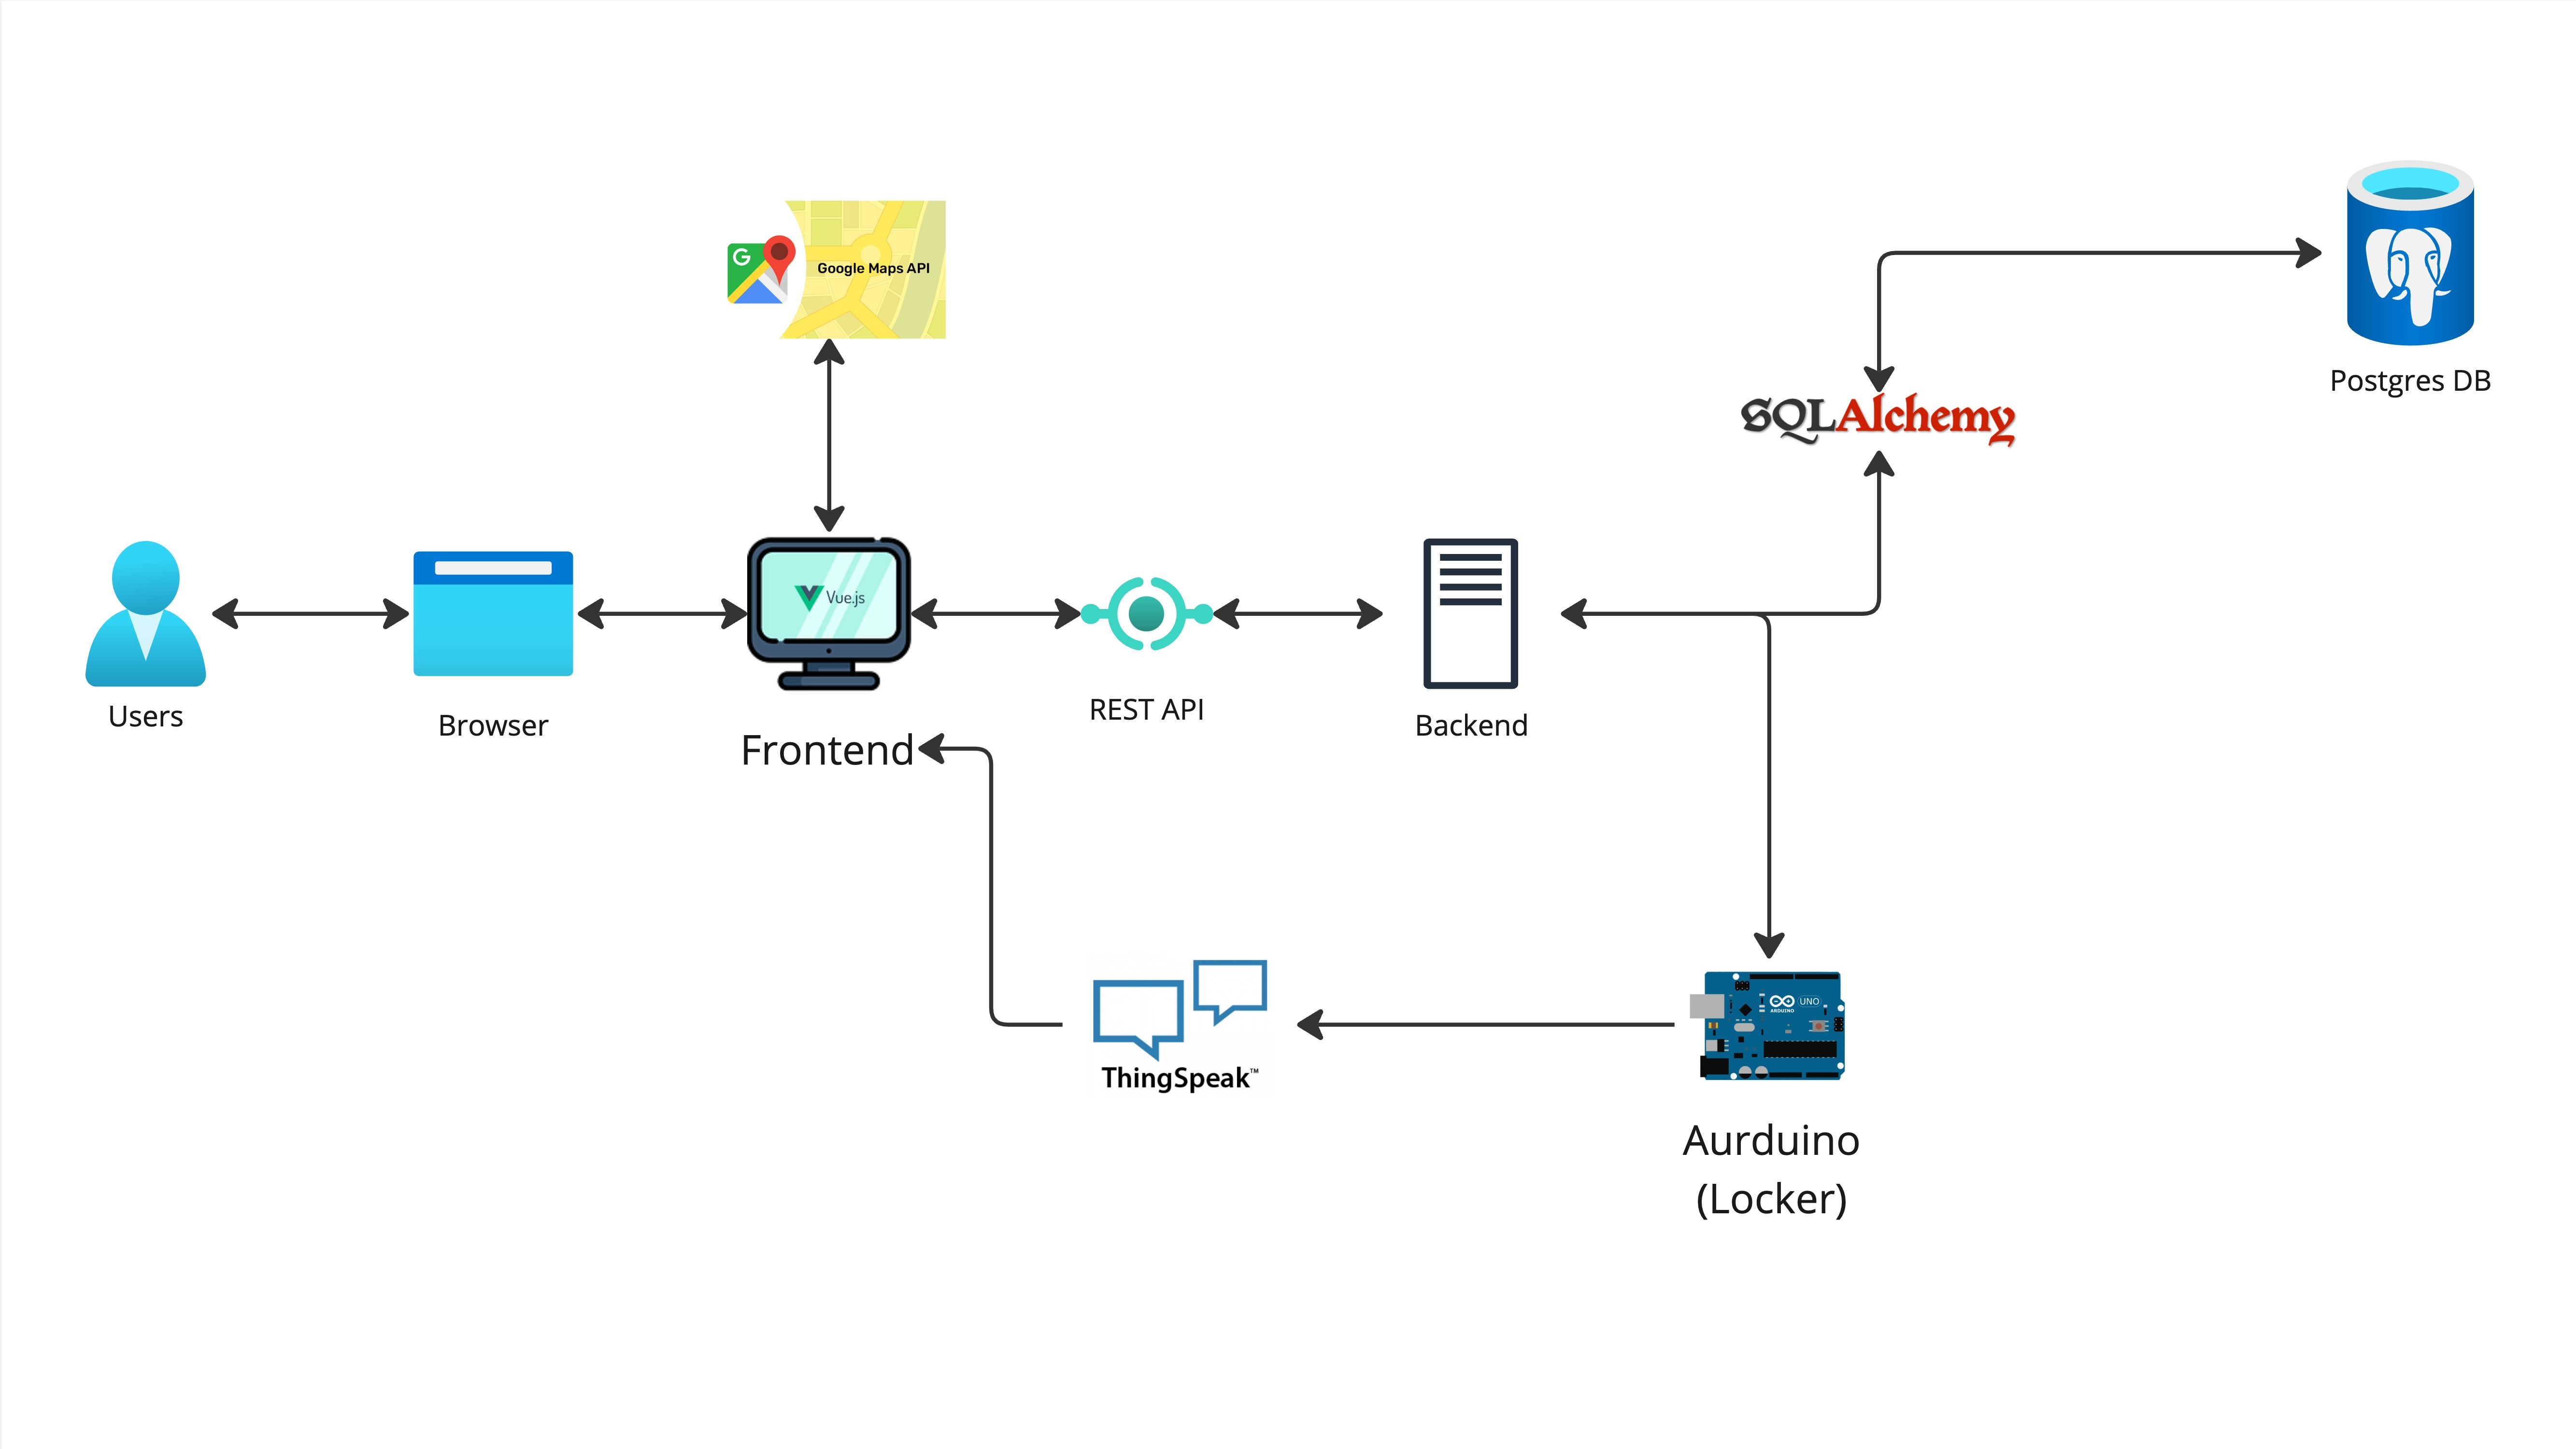
\includegraphics[width=\textwidth]{images/software_design_diagram}
    \caption{Software Design Diagram}
    \label{fig:software_design}
\end{figure}



The image above depicts a high-level overview of the software design architecture,
illustrating the interaction between various components and their roles within the system.
Throughout this chapter, we elucidate the rationale behind each architectural decision
and technology selection, elucidating their benefits and contributions to the overall
functionality and performance of the locker system.

Now, let's delve into the intricacies of the software design, beginning with an exploration
of the architectural approach adopted for the project.


\subsection{Architectural Approach}

The adoption of a modern microservices architecture, with clear separation between
frontend and backend components, offers several advantages for the locker system project.
By decoupling these layers and enabling communication via a RESTful API, we achieve enhanced
modularity, scalability, and flexibility. This modular approach facilitates
independent development and deployment of frontend and backend services, enabling
rapid iteration and evolution of the system. Moreover, the RESTful API design simplifies
integration with third-party services and future expansion of functionality, ensuring
adaptability to changing requirements and technological advancements.

\subsection{Frontend Technologies}

Vue.js was selected as the frontend framework due to its lightweight nature, simplicity,
and extensive ecosystem of plugins and libraries. Its reactive data binding and component-based
architecture enable the creation of dynamic and interactive user interfaces, enhancing
the user experience. Additionally, the integration of Tailwind CSS and Bootstrap provides
a comprehensive set of styling utilities and pre-designed components, enabling rapid
prototyping and ensuring consistent design across different devices and screen sizes.
The use of these frontend technologies not only accelerates development but also enhances
maintainability and scalability, making them well-suited for a complex application like
the locker system.

\subsection{Google Maps Integration}

The integration of the Google Maps API enriches the user experience by providing visual
representation of locker locations. This feature enhances user convenience and navigation,
particularly in large university campuses where locker locations may not be readily apparent.
By leveraging the Google Maps API, users can easily locate their rented devices, thereby
reducing frustration and improving overall satisfaction with the service.

\subsection{Backend Technologies}

FastAPI was chosen as the backend framework due to its high performance,
asynchronous capabilities, and intuitive API design. Its built-in support for
asynchronous programming enables efficient handling of concurrent requests,
ensuring optimal responsiveness and scalability, especially under heavy loads.
Additionally, FastAPI's automatic generation of OpenAPI documentation simplifies
API documentation and client integration, enhancing developer productivity and collaboration.
The use of FastAPI aligns with industry best practices and standards, ensuring the reliability,
security, and maintainability of the locker system backend.

\subsection{Database Management}

The utilization of SQLAlchemy as the ORM tool offers numerous benefits for database management
within the locker system project. By abstracting away the complexities of database interaction,
SQLAlchemy enhances developer productivity and code maintainability,
while also mitigating the risk of SQL injection vulnerabilities. Furthermore,
Alembic provides seamless database schema versioning and migration capabilities,
facilitating continuous evolution and refinement of the database schema over time.
These features ensure data integrity, consistency, and scalability, making SQLAlchemy
and Alembic well-suited for managing the relational database backend of the locker system.

\subsection{Database Choice}

PostgreSQL was selected as the underlying database management system for its robustness,
reliability, and advanced feature set. Its support for ACID transactions,
data integrity constraints, and extensible data types ensures the consistency and
integrity of stored data, critical for a mission-critical application like the locker system.
Additionally, PostgreSQL's scalability and performance optimizations make it capable
of handling large volumes of concurrent transactions and complex queries, making it an ideal
choice for the storage and retrieval of locker rental and user data.

\subsection{Locker Controls}

The integration of Arduino-based locker controls provides a cost-effective and
customizable solution for managing locker access and device rentals. Arduino's open-source
hardware platform, coupled with its rich ecosystem of sensors and actuators, enables the
implementation of tailored locker control mechanisms suited to the specific requirements of
the locker system. By exposing REST APIs for communication with the backend, Arduino controllers
facilitate real-time updates and authentication checks, ensuring secure and reliable access to
rented devices.

\subsection{Charging Data Management}

ThingSpeak serves as an IoT analytics platform for collecting, storing, and visualizing
charging data generated by the Arduino controllers. Its cloud-based infrastructure and
user-friendly interface simplify data management and analysis, enabling administrators to
monitor charging activities and usage patterns in real-time. The integration of ThingSpeak
with the frontend enables the seamless transmission of processed data for visualization,
empowering administrators to make informed decisions regarding resource allocation and system
optimization.

\subsection{Hosting and Deployment}

The successful deployment and hosting of the locker system components are crucial for ensuring accessibility, scalability, and reliability. In this section, we elucidate the deployment strategies employed for the frontend, backend, and database components, leveraging cloud-based solutions and containerization technologies for seamless deployment and management.

\begin{figure}[h]
    \centering
    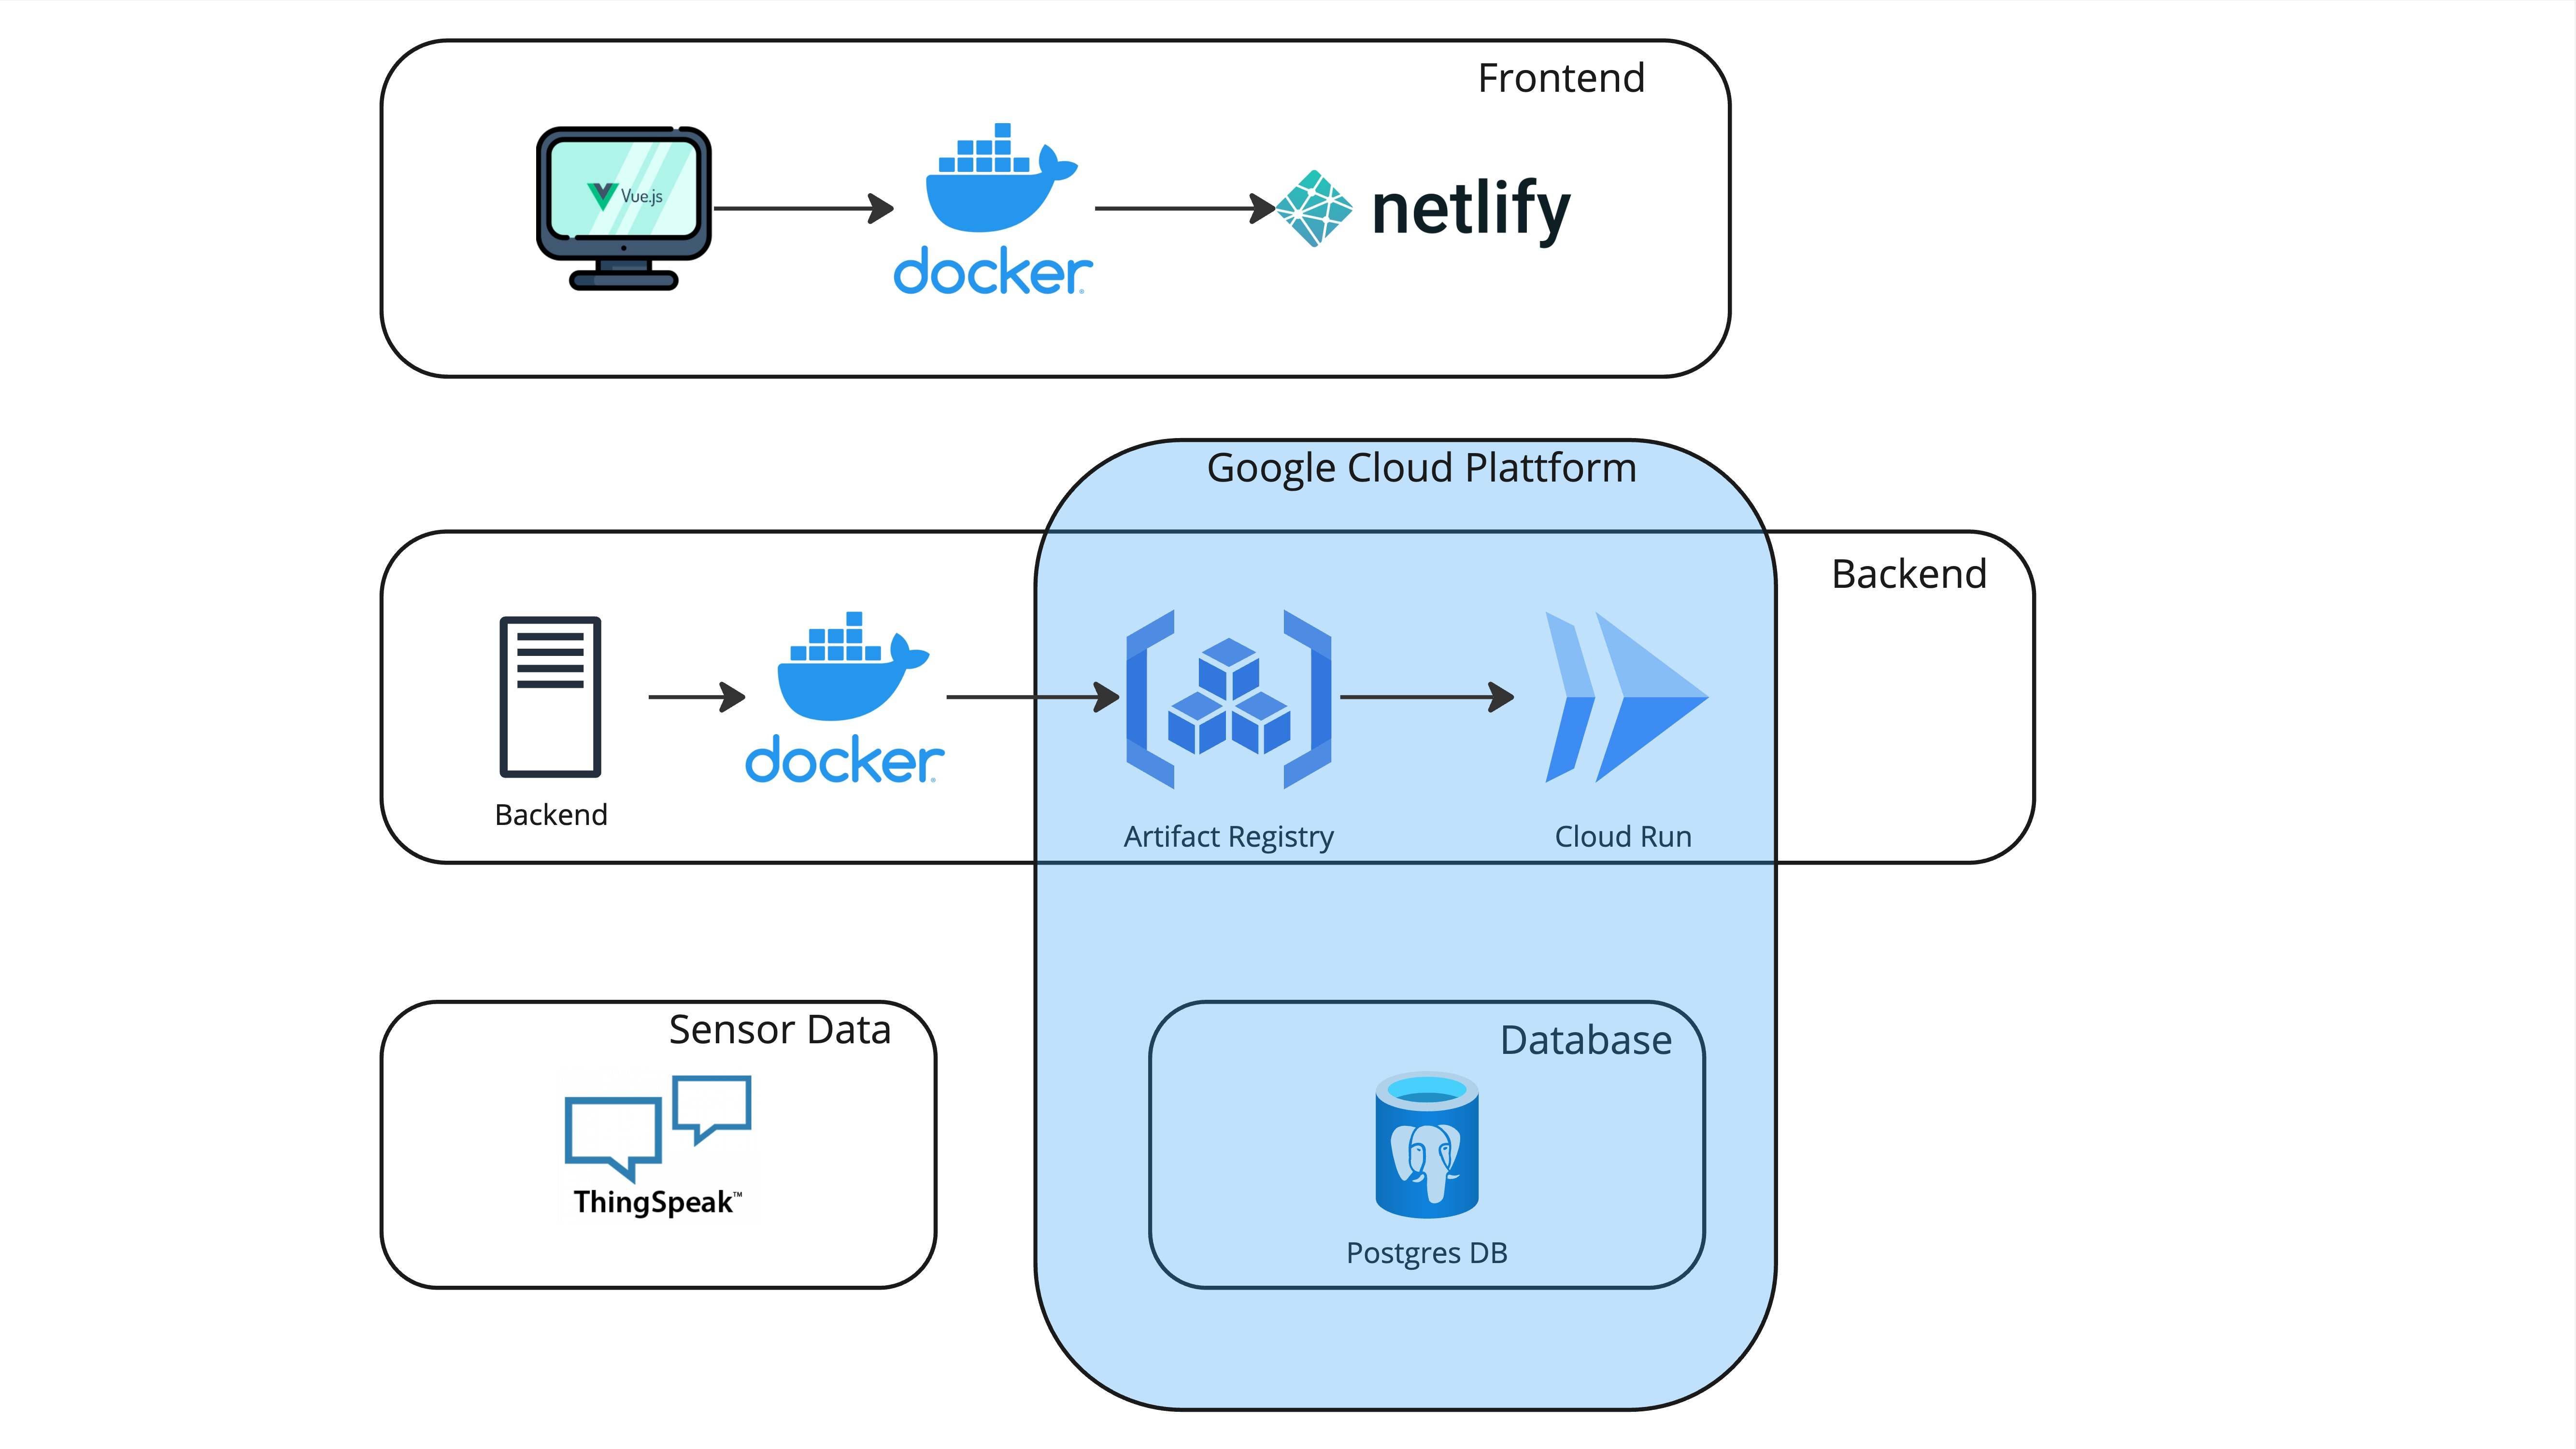
\includegraphics[width=\textwidth]{images/software_design_deployment}
    \caption{Overview of Deployment Processes}
    \label{fig:deployment_overview}
\end{figure}

\subsubsection{Frontend Deployment}

The frontend of the locker system is packaged into a Docker container to encapsulate its dependencies and environment. This containerized approach ensures consistency and portability across different environments, mitigating potential compatibility issues. Subsequently, the Docker container is deployed to Netlify, a popular platform for hosting static websites and web applications. Netlify provides a straightforward deployment process, seamless integration with Git repositories, and automatic build and deployment pipelines. Additionally, Netlify assigns a public address to the deployed frontend, enabling users to access the locker system via the internet with ease.

\subsubsection{Backend Deployment}

Similar to the frontend, the backend services are containerized using Docker to streamline deployment and management. Once the backend Docker image is built, it is pushed to Google Cloud's Artifact Registry, a managed service for storing container images securely. Artifact Registry ensures version control, access control, and image vulnerability scanning, enhancing the security and reliability of the deployment process. Subsequently, the containerized backend services are deployed to Google Cloud Run, a fully managed serverless platform for running containerized applications. Google Cloud Run automatically scales the backend services based on demand, ensuring optimal performance and cost-efficiency. Furthermore, Google Cloud Run assigns a public address to the deployed backend services, facilitating seamless communication with the frontend and other system components over the internet.

\subsubsection{Database Hosting}

The PostgreSQL database used by the locker system is hosted on Google Cloud SQL, a fully managed relational database service. Google Cloud SQL offers automatic backups, high availability, and scalability, relieving the burden of database administration and maintenance. By leveraging Google Cloud SQL, we ensure data durability, reliability, and performance, critical for the storage and retrieval of locker rental and user data. Additionally, Google Cloud SQL provides seamless integration with other Google Cloud services, simplifying data management and access control.

\subsubsection{Sensor Data Management}

The sensor data collected by the Arduino controllers is transmitted to ThingSpeak, a cloud-based IoT analytics platform. ThingSpeak provides a scalable and reliable infrastructure for storing, analyzing, and visualizing sensor data in real-time. As a Software as a Service (SaaS) solution, ThingSpeak eliminates the need for hosting and infrastructure management, allowing developers to focus on application logic and data analysis. By leveraging ThingSpeak, we ensure efficient management and utilization of the sensor data.

\subsection{Conclusion}

In summary, the deployment and hosting of the locker system components leverage cloud-based solutions and containerization technologies to ensure accessibility, scalability, and reliability. By utilizing platforms such as Netlify, Google Cloud, and ThingSpeak, we streamline the deployment process, enhance security and performance, and enable seamless integration between different system components. This comprehensive approach to hosting and deployment underscores the importance of utilizing cloud-native technologies and services for building robust and scalable applications in modern computing environments.

The software design of the locker system incorporates a carefully selected set of technologies and architectural principles tailored to the specific requirements and challenges of managing locker rentals and device access in university environments. Many of these technologies were introduced in lectures at our university, and while there may be other options available, we opted for those recommended by the university and with which we had prior experience. By leveraging modern frameworks, platforms, and best practices, the system delivers enhanced functionality, scalability, and user experience, ensuring its effectiveness and viability in real-world deployments.


\section{Frontend}
{\tiny Written by: Philipp Becker}
\subsection{Frontend Implementation}\label{sec:Frontend_Implementation}

This subsection provides an overview of the implementation details for the front end of the locker system. It deals with the technologies, frameworks and development environment in use in the development process.

\subsubsection{Project Setup}

The frontend of our locker system utilizes Vue.js, equipped with auxiliary libraries such as Vue Router for routing,  BootstrapVue3 for interface design, chosen for their robustness and effective integration capabilities.

\paragraph{Development Environment Preparation}
Node.js is requisite for utilizing npm, which manages the project's dependencies. The project is cloned from its repository, which includes essential configuration files like \texttt{package.json}.

\paragraph{Dependencies and Local Server}
In the project directory, dependencies are installed via \texttt{npm install}, incorporating Vue Router and BootstrapVue3. The local development server is initiated with \texttt{npm run dev}, providing a live-reload feature beneficial during development.

\paragraph{Configuration and Build}
Environment variables are configured to manage API endpoints effectively. The \texttt{npm run build} command compiles the application into a 'dist' folder, segmenting it into optimized chunks that improve load efficiency, ideal for deployment.

\paragraph{Quality Assurance}
Integration of ESLint and Prettier ensures code quality and consistency, essential for maintaining high standards in collaborative development environments.

This setup process outlines a systematic approach to preparing a scalable and efficient development environment for the Vue.js frontend, aligned with contemporary web development best practices.

\subsubsection{Project Structure}

This section outlines the structural framework of the Vue.js application, focusing on the core components that define its architecture. A well-organized project structure is crucial for efficient development and maintenance.

\begin{itemize}
    \item \textbf{README.md}: This file serves as the project's main documentation hub, containing comprehensive information on setup instructions, deployment steps, and other essential details. A well-written README enhances project understanding and facilitates collaboration among team members.

    \item \textbf{Main.ts}: The entry point for the Vue application. This file initializes the root Vue instance, sets up the initial plugins, dependencies, and mounting point for the app to the DOM.

    \item \textbf{App.vue}: The main Vue component that acts as the root of the application. It integrates the primary structure or layout and serves as the entry point for the component hierarchy.

    \item \textbf{components}: This directory houses reusable Vue components that can be utilized across different parts of the application, such as buttons, input fields, and dialogs, helping to maintain a clean and modular structure.

    \item \textbf{views}: Contains Vue components that represent different pages or routes of the application. These are typically larger and more complex than simple components and form the main parts of the application interface.

    \item \textbf{router}: Manages the routing configuration for the application. It defines the routes and their corresponding components, enabling navigation between different views within the application.

    \item \textbf{assets}: This directory stores static resources such as images, stylesheets, and fonts that are used by the application. It helps in organizing and managing the UI resources that are not part of Vue component logic.
\end{itemize}

\subsubsection{Vue.js Imports and Mounting}
\begin{itemize}
    \item \textbf{Imports and Styles Configuration:} The Main.ts file plays a crucial role in setting up the Vue.js application by importing essential libraries and styles. It includes the Vue framework, the main component App.vue, the router, and Pinia for state management. For the user interface, BootstrapVue3 and Bootstrap icons are imported along with their respective CSS files to ensure the application is both functional and aesthetically pleasing.
    \begin{lstlisting}
import { createApp } from 'vue';
import App from './App.vue';
import router from './router';
import BootstrapVue3 from 'bootstrap-vue-3';
import { BootstrapIconsPlugin } from "bootstrap-icons-vue";
import './css/index.css';
import 'bootstrap/dist/css/bootstrap.css';
import 'bootstrap-vue-3/dist/bootstrap-vue-3.css';
    \end{lstlisting}

    \item \textbf{Application Setup and Mounting:} After importing the necessary modules, the application is instantiated and configured in Main.ts. Key steps include setting global properties like the backend link, and integrating BootstrapVue3, Bootstrap icons and the router. The application is then mounted to the DOM at the 'app' selector, initializing the system's frontend.
    \begin{lstlisting}
const app = createApp(App)
app.config.globalProperties.backendLink = 'https://f-itplfo6nya-uc.a.run.app'
app.use(BootstrapVue3)
app.use(BootstrapIconsPlugin)
app.use(router)
app.mount('#app')
    \end{lstlisting}
\end{itemize}
\subsubsection{Vue.js-File Introduction}
In vue.js, individual vue files are divided into three parts. These start with a template part, followed by a script part and optionally a style part can be created.
The html code is written in the template part. However, libraries such as BootstrapVue can also be used in this part to use ready-made HTML elements. In the script part, the page is initialized and all functions that this special page uses can be defined. Comprehensive functions are integrated in the import of the script part. If it is necessary to style html elements differently on a specific page, a style section can be added in which css classes can be defined.
\begin{itemize}
\item \textbf{template:}
\begin{lstlisting}
<template>
  <div class="mx-auto my-10" style="width: 90%;">
    <h3 class="text-left">Admin Dashboard</h3>
    <dashboard-charts></dashboard-charts>
    <div class="d-flex justify-content-center align-items-center pt-10">
      <iframe width="450" height="260" style="border: 1px solid #cccccc;" src="https://thingspeak.com/channels/2530450/widgets/852176"></iframe>

      <iframe width="450" height="260" style="border: 1px solid #cccccc;" src="https://thingspeak.com/channels/2530450/charts/1?bgcolor=%23ffffff&color=%23d62020&dynamic=true&results=60&title=History+of+Wattage&type=line"></iframe>
    </div>

    <div class="flex justify mt-4">
    </div>
  </div>
</template>
    \end{lstlisting}

\item \textbf{script:}
\begin{lstlisting}
<script lang="ts">
import { defineComponent } from 'vue';
import DashboardCharts from '@/components/DashboardCharts.vue';

export default defineComponent({
  components: {
    DashboardCharts,
  },
  setup() {

    return {
    }
  },
})
</script>
    \end{lstlisting}
\item \textbf{style:}
\begin{lstlisting}
</script>
<style>
.pin-container {
  display: flex;
  justify-content: center;
  font-family: Arial, sans-serif;
</style>
    \end{lstlisting}
\end{itemize}

\subsubsection{Vue Components}
Vue components can be created as vue files and can therefore be imported and used on any vue screen. The following example shows our footer, which is then integrated into the template part of a sample vue.

\begin{lstlisting}
<template>
  <footer class="footer bg-light text-center text-lg-start">
    <div class="container p-4">
      <div class="row">
        <div class="col-lg-6 col-md-12 mb-4 mb-md-0">
          <h5 class="text-uppercase">Database Inventory Locker System</h5>
          <p>We provide your favorite Tools for rent.</p>
          <p>Your Devices are safe and charged after storing.</p>
        </div>
        <div class="col-lg-6 col-md-12 mb-4 mb-md-0 text-lg-end">
          <h5 class="text-uppercase">Follow Us on Social Media</h5>
          <p>
            <span class="p-2" style="font-size: 24px;">Icon1</span>
            <span class="p-2" style="font-size: 24px;">Icon2</span>
          </p>
        </div>
      </div>
    </div>

    <div class="text-center p-3" style="background-color: rgba(0, 0, 0, 0.05);">
    2024
      <a class="text-dark" href="https://databaseinventorysystem.com/">databaseinventory.com</a>
    </div>
  </footer>
</template>

    \end{lstlisting}
Usage of the Component
    \begin{lstlisting}
<template>
  <Footer_component></footer_component>
</template>
#Import 
<script>
import Footer_component from "@/components/footer_component.vue";
</script>
    \end{lstlisting}

\subsubsection{Implementing Role-Based Access Control}
The useLoggedIn composable encapsulates the management of user authentication states within a Vue.js application, utilizing Vue's reactive system. This composable serves as a centralized mechanism to manage and react to changes in the user's login status, which is pivotal in implementing role-based access controls (RBAC). Below, the functionality and internal mechanisms of the useLoggedIn composable are dissected and explained:

\begin{itemize}
\item \textbf{Composition Function}
The useLoggedIn function exports a reactive reference, loggedIn, initialized to "None", indicating no user is currently authenticated. The function returns an object containing this reactive state alongside functions setLoggedIn and checkLoggedIn, which manipulate and assess the authentication state, respectively.
\begin{lstlisting}[]
import { type Ref, ref } from "vue";
export type LoggedIn = "Admin" | "User" | "None";
const loggedIn: Ref<LoggedIn> = ref("None");
export const useLoggedIn = () => {
    return {
        loggedIn,
        setLoggedIn,
        checkLoggedIn,
    };
}
\end{lstlisting}
\item \textbf{Check Login Status}
The checkLoggedIn method evaluates the user's role by reading the sessionStorage where the user's role is persisted across sessions. Depending on the stored value, it sets the loggedIn state to "Admin", "User", or "None", effectively updating the authentication status based on session data.

\begin{lstlisting}[]
const checkLoggedIn = () => {
    if (sessionStorage.getItem("isAdmin") === "true") {
        loggedIn.value = "Admin";
    } else if (sessionStorage.getItem("isAdmin") === "false") {
        loggedIn.value = "User";
    } else {
        loggedIn.value = "None";
    }
};
\end{lstlisting}
\item \textbf{Set Login Status}
The setLoggedIn function is used to explicitly set the authentication status. It updates the sessionStorage to reflect the new role ("Admin" or "User") or clears it if logging out. This method also updates the reactive loggedIn state, triggering any dependent components to re-render based on the new authentication status.

\begin{lstlisting}[]
const setLoggedIn = (l: LoggedIn) => {
    console.log(l);
    if (l == "Admin") {
        sessionStorage.setItem("isAdmin", "true");
    } else if (l == "User") {
        sessionStorage.setItem("isAdmin", "false");
    }
    else{
        sessionStorage.removeItem('isAdmin');
    }
    loggedIn.value = l;
};
\end{lstlisting}
\end{itemize}

\subsubsection{Sitemap Overview}
This section presents the sitemaps for both the Admin and User frontends of our system. These sitemaps are visual representations that detail the structure and navigational schema of the respective interfaces. By examining these sitemaps, one can gain a comprehensive understanding of the user flow and interaction design implemented in both the administrative and user-facing sections of the application.
\begin{itemize}
\item \textbf {Admin Frontend}
\begin{figure}[h]
    \centering
    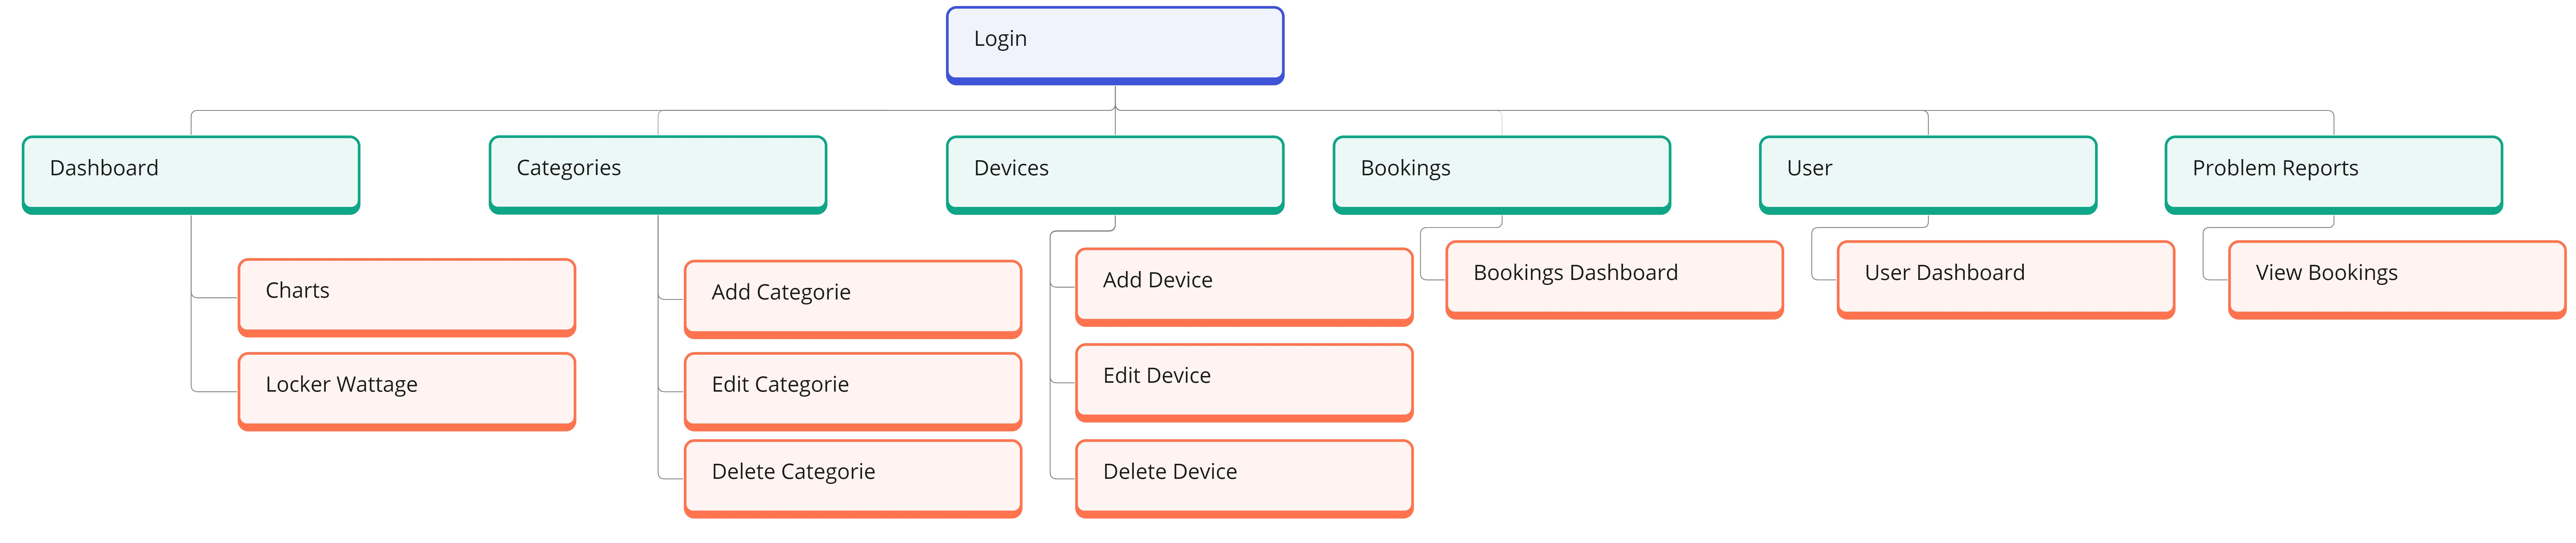
\includegraphics[width=1\textwidth]{images/Sitemap.jpg}
    \caption{Admin Frontend Sitemap}
    \label{fig:myimage}
\end{figure}
\clearpage
\item \textbf {User Frontend}
\begin{figure}[h]
    \centering
    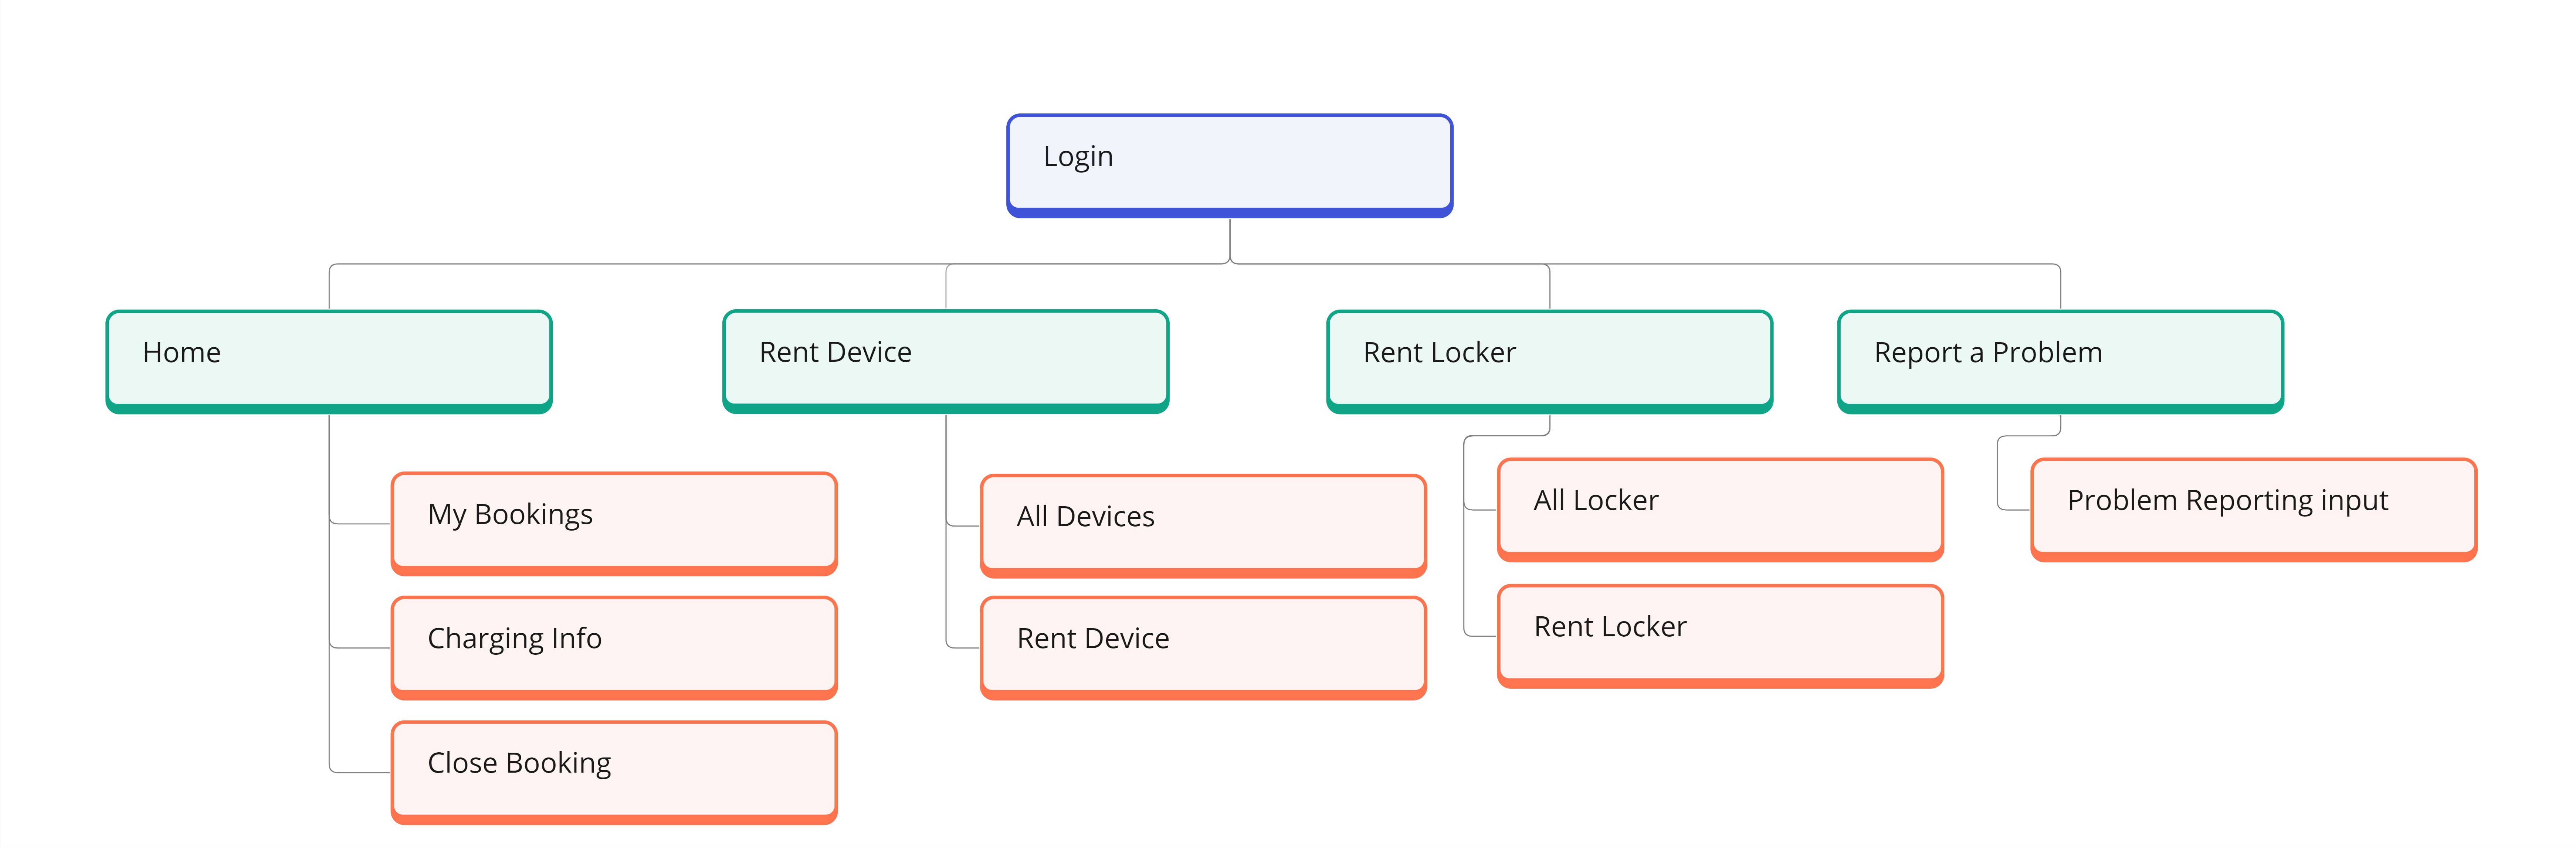
\includegraphics[width=1\textwidth]{images/usersitemap.jpg}
    \caption{User Frontend Sitemap}
    \label{fig:myimage}
\end{figure}
\end{itemize}

\subsubsection{Frontend Demo Screenshots}
This section provides a visual demonstration of the frontend interface, starting with the Admin-Portal Dashboard. 
\begin{itemize}
\item \textbf {Admin Dashboard:} The dashboard offers a comprehensive overview of all device bookings and displays revenue statistics for recent months. Additionally, in alignment with our commitment to security awareness, the dashboard includes a wattage overview for the currently booked lockers.
\begin{figure}[h]
    \centering
    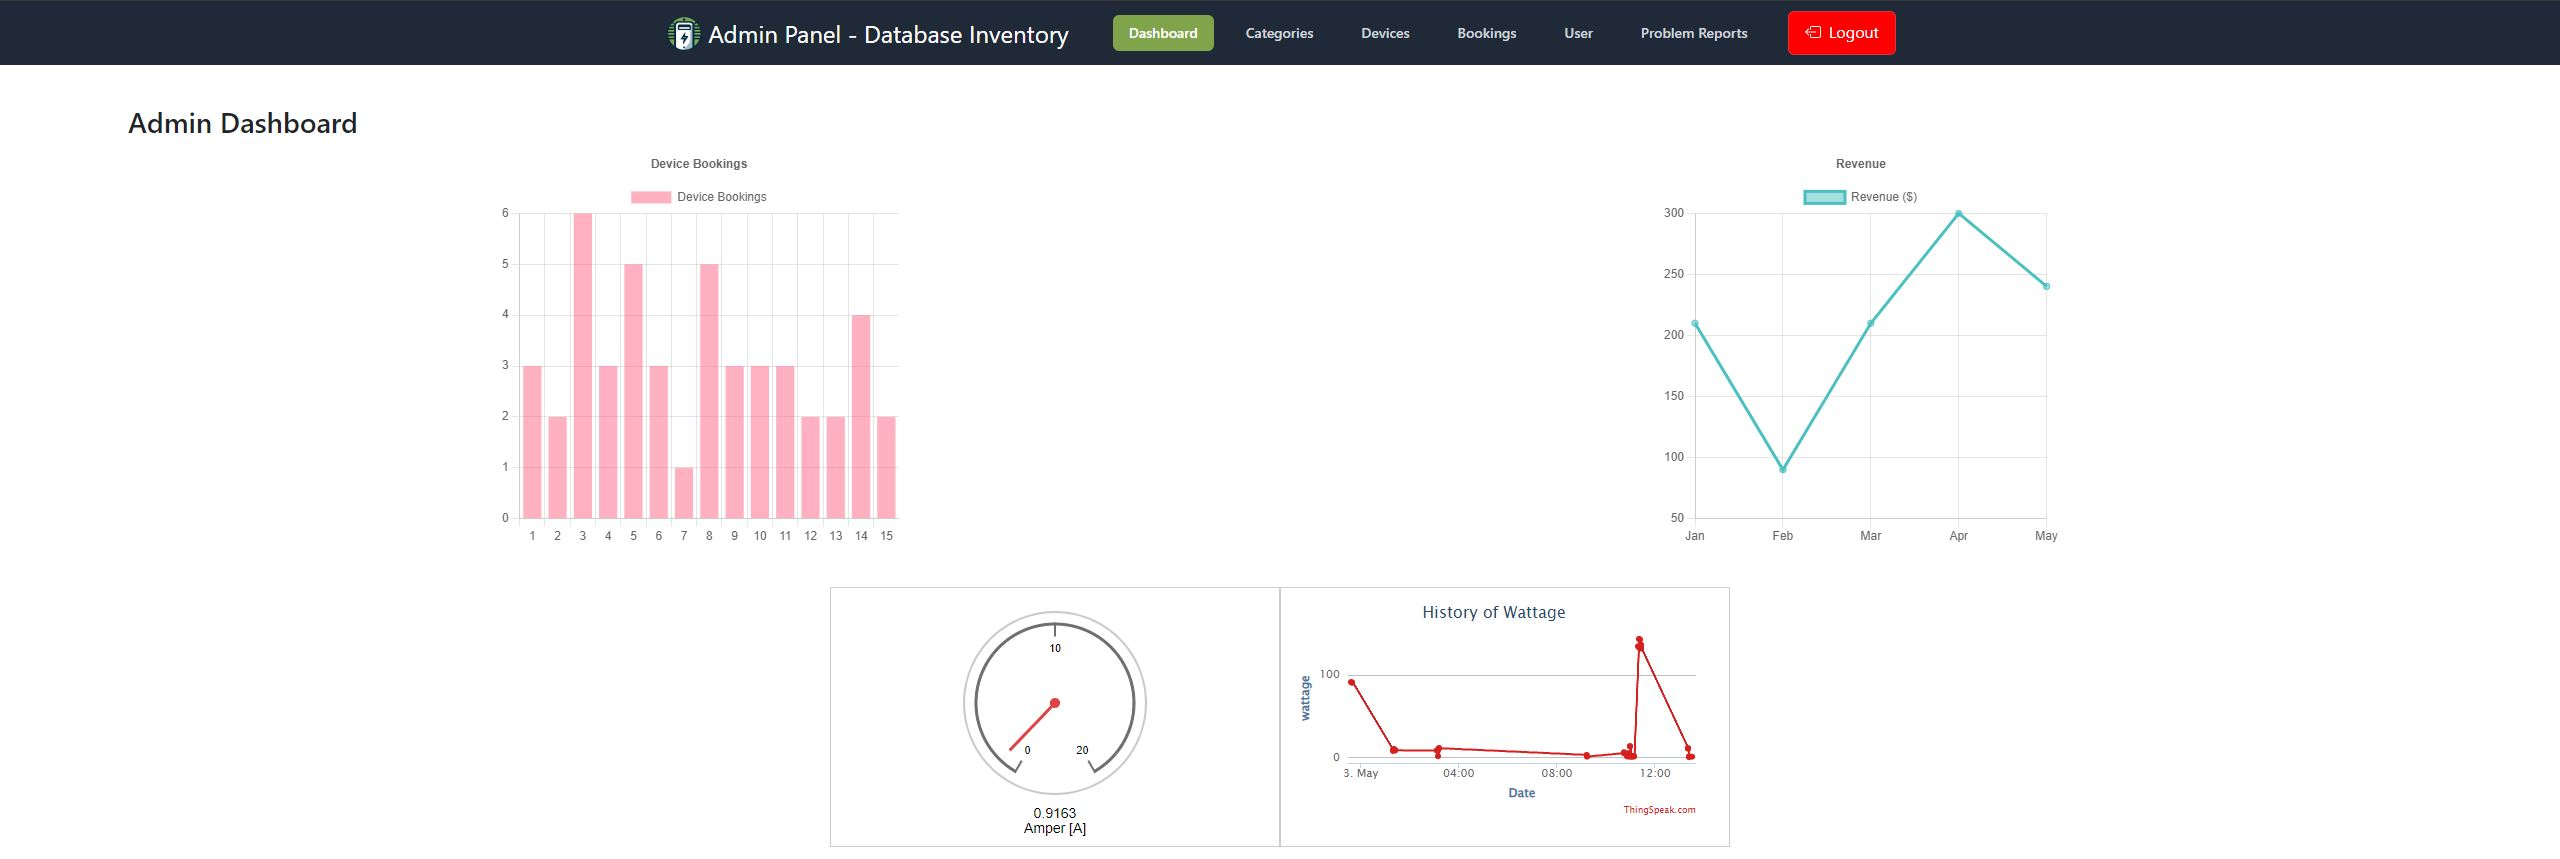
\includegraphics[width=1\linewidth]{images/admin-dashboard.JPG}
    \caption{Admin Dashboard}
    \label{fig:admin-dashboard}
\end{figure}

\item \textbf {Categories Screen:}In the Categories Screen, administrators can view all categories that have been added to the system. Each category can be edited or deleted, and new categories can be added, providing flexible management of the system's categorization logic.
\begin{figure}[h]
    \centering
    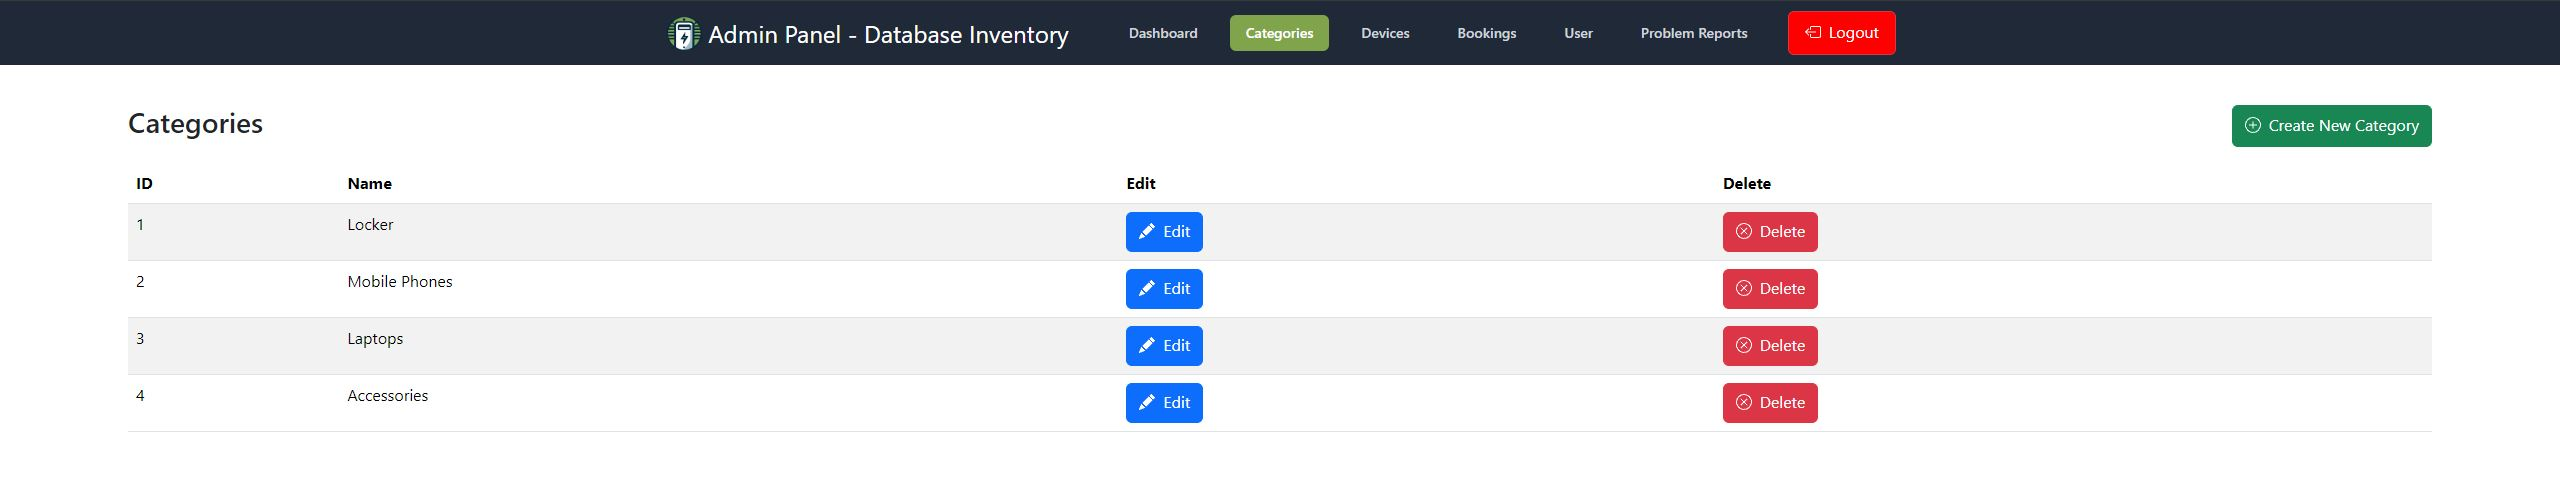
\includegraphics[width=1\linewidth]{images/categories.JPG}
    \caption{Admin Dashboard Categories}
    \label{fig:categories-dashboard}
\end{figure}


\item \textbf {Edit Categories Screen:}This figure depicts the Edit Category Modal, where administrators can easily modify the name of a category, enhancing the adaptability of system configurations.
\begin{figure}[h]
    \centering
    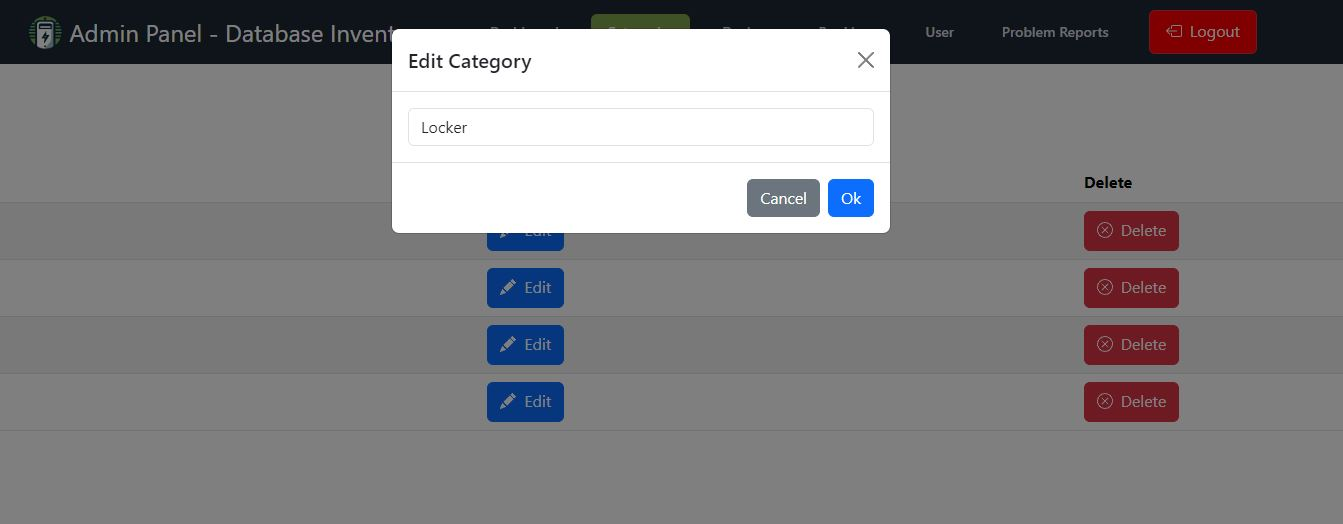
\includegraphics[width=1\linewidth]{images/edit categorie.JPG}
    \caption{Admin Dashboard Edit Categories Modal}
    \label{fig:edit-category-modal}
\end{figure}


\item \textbf {Devices Screen:}The Devices Screen displays all devices that have been integrated into the system. This interface allows for the addition of new items and the modification of existing devices, ensuring that the system remains up-to-date and functional.
\begin{figure}[h]
    \centering
    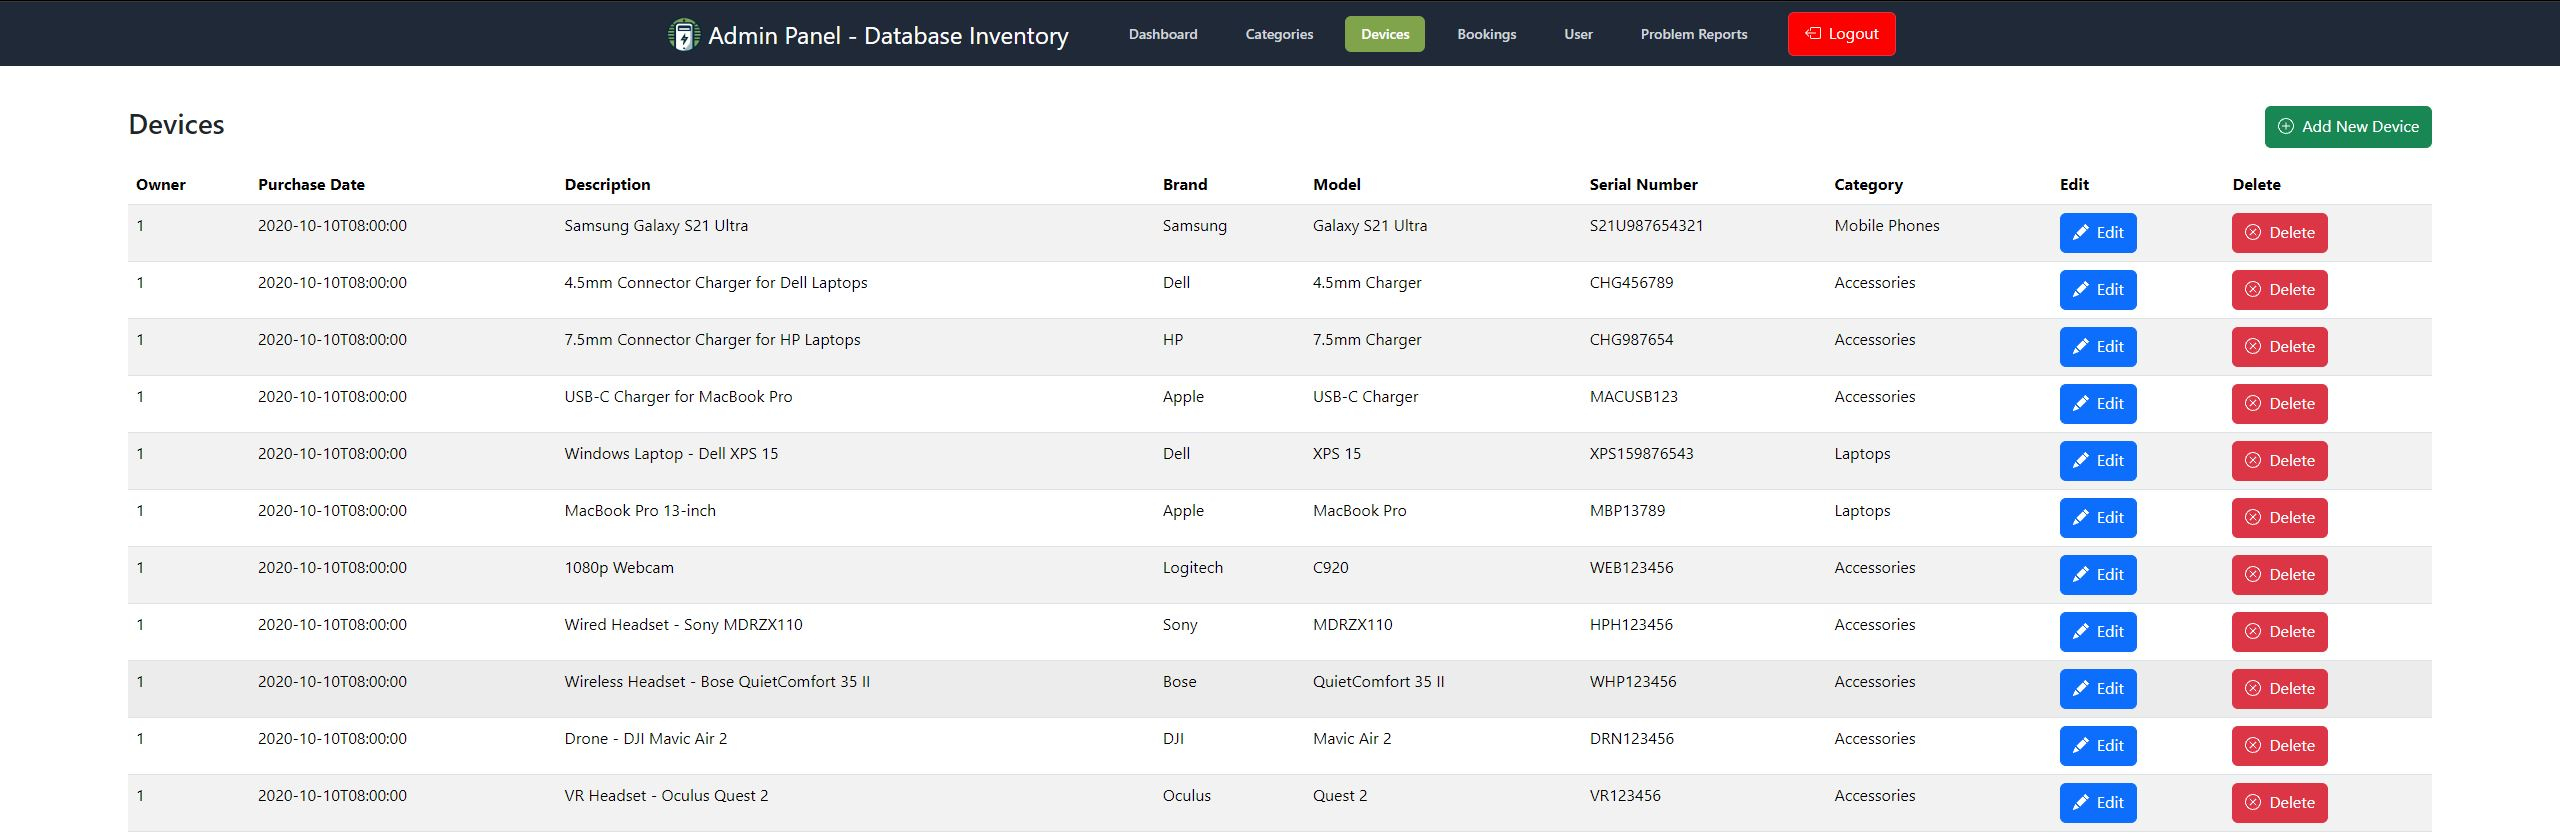
\includegraphics[width=1\linewidth]{images/devices.JPG}
    \caption{Admin Dashboard Devices}
    \label{fig:devices-dashboard}
\end{figure}

\item \textbf {Problem Reports Screen:}At the Problem Reports screen, administrators can review all user-submitted reports. Each report includes a photograph and is linked to the booking it pertains to, allowing for efficient and effective issue tracking and resolution.
\begin{figure}[h]
    \centering
    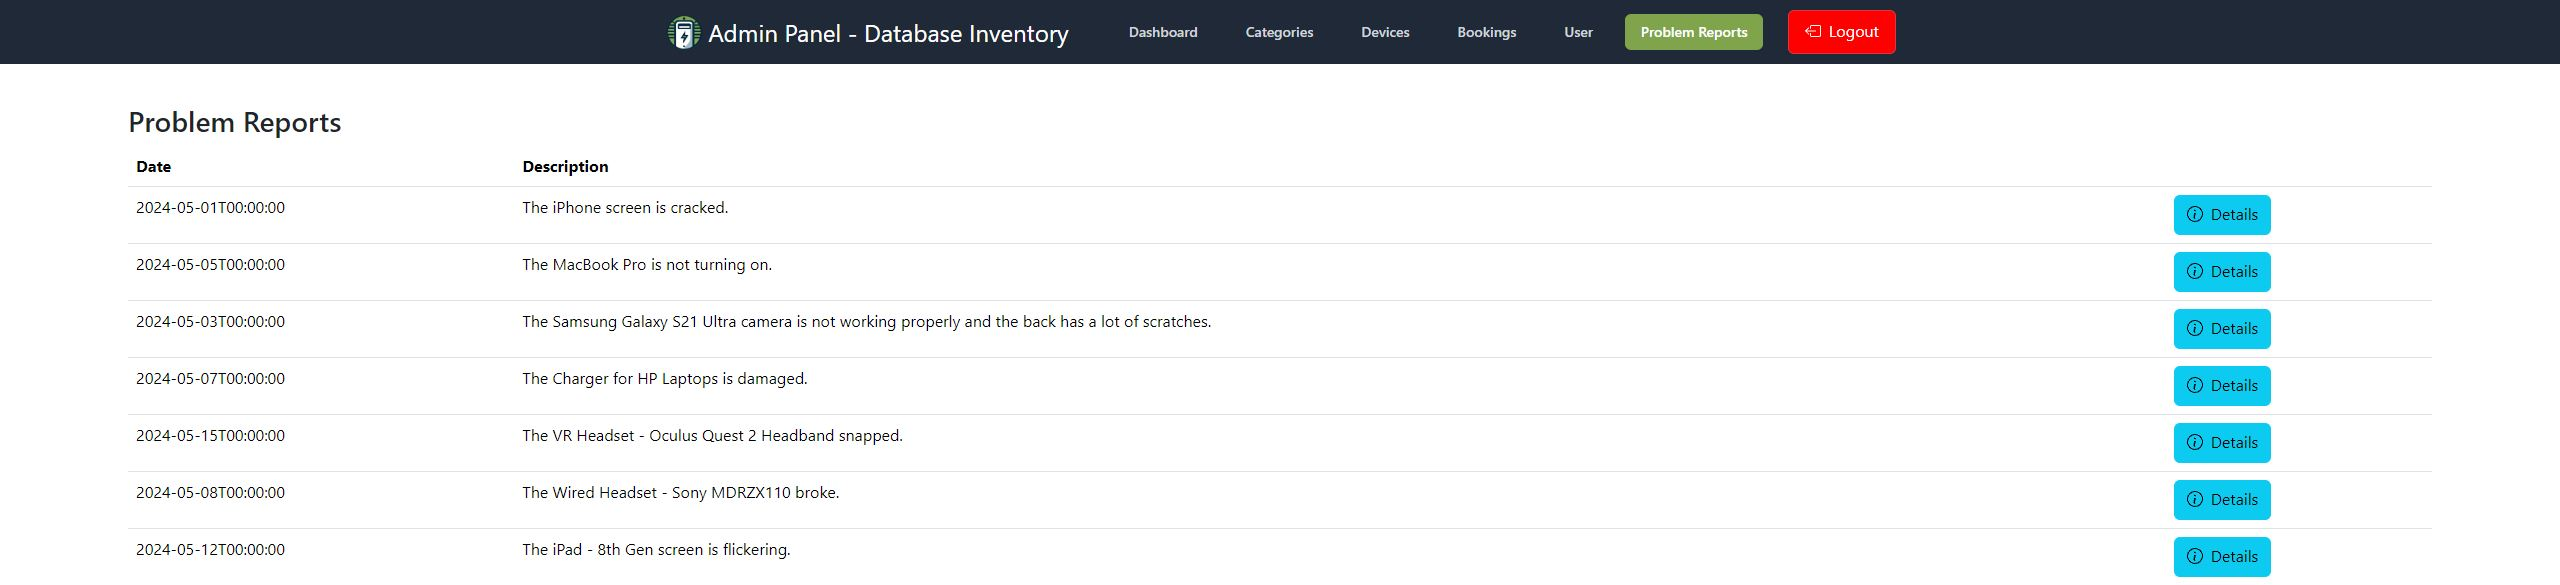
\includegraphics[width=1\linewidth]{images/problem reports.JPG}
    \caption{Admin Dashboard Problem Reports}
    \label{fig:problem-reports-dashboard}
\end{figure}
\newpage
\item \textbf{User Frontend Bookings:} This interface allows users to view all their bookings. It provides detailed information for each booking, including price, start and end times. Users can also terminate an ongoing booking directly from this screen. Additionally, for lockers rented for charging, a 'wattage' button is available to monitor power usage.
\begin{figure}[h]
    \centering
    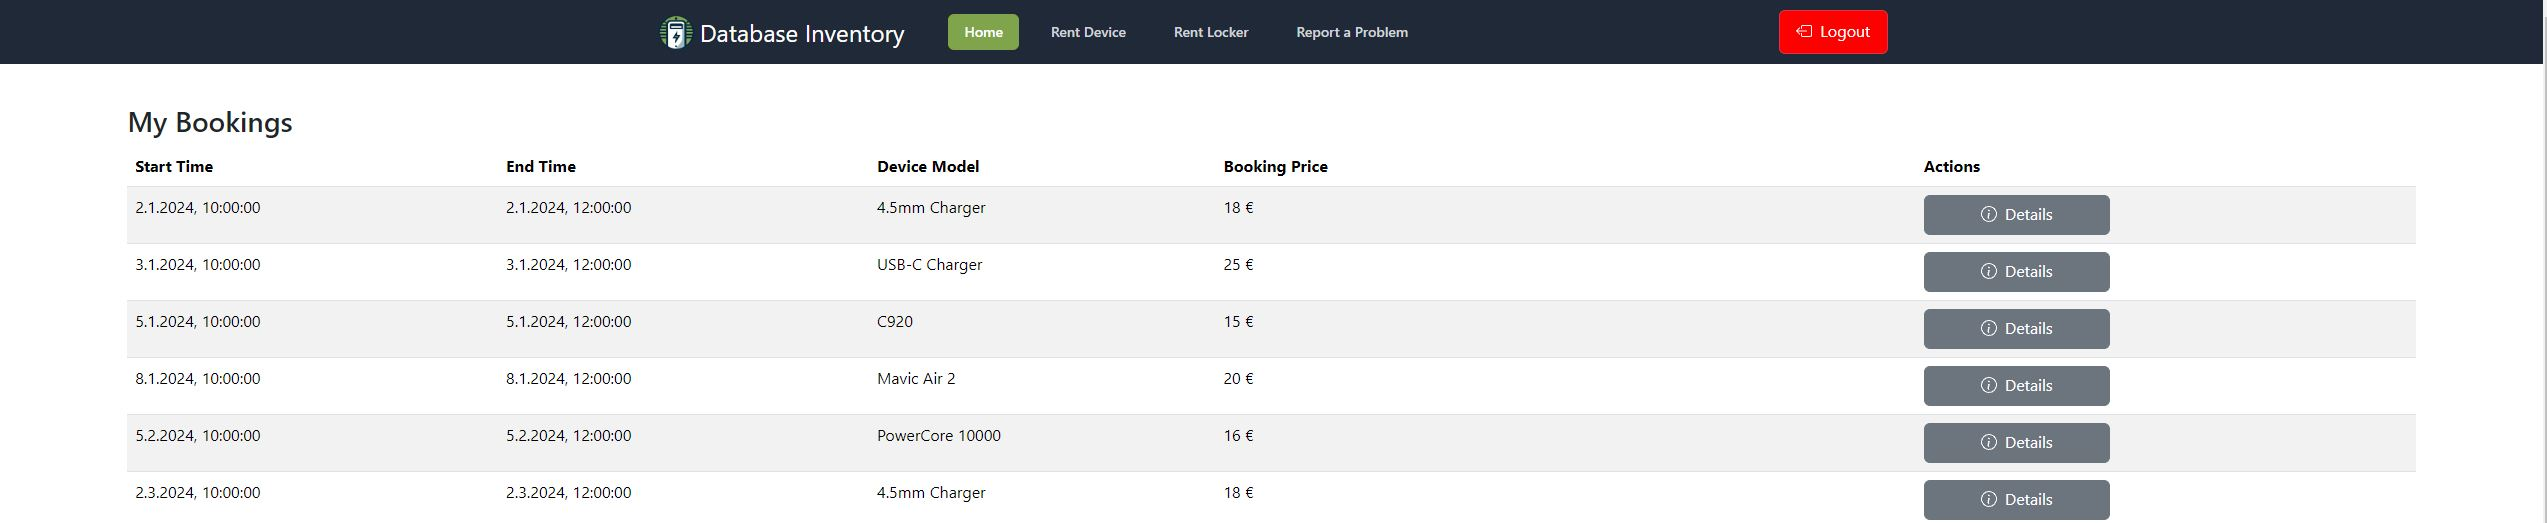
\includegraphics[width=1\linewidth]{images/bookings.JPG}
    \caption{User Frontend Bookings}
    \label{fig:user-bookings-dashboard}
\end{figure}

\item \textbf{User Frontend Rent Device:} This screen displays all available devices for rent, detailing the cost per hour and providing comprehensive information about each device. Users can select devices based on their specific needs and availability.
\begin{figure}[h]
    \centering
    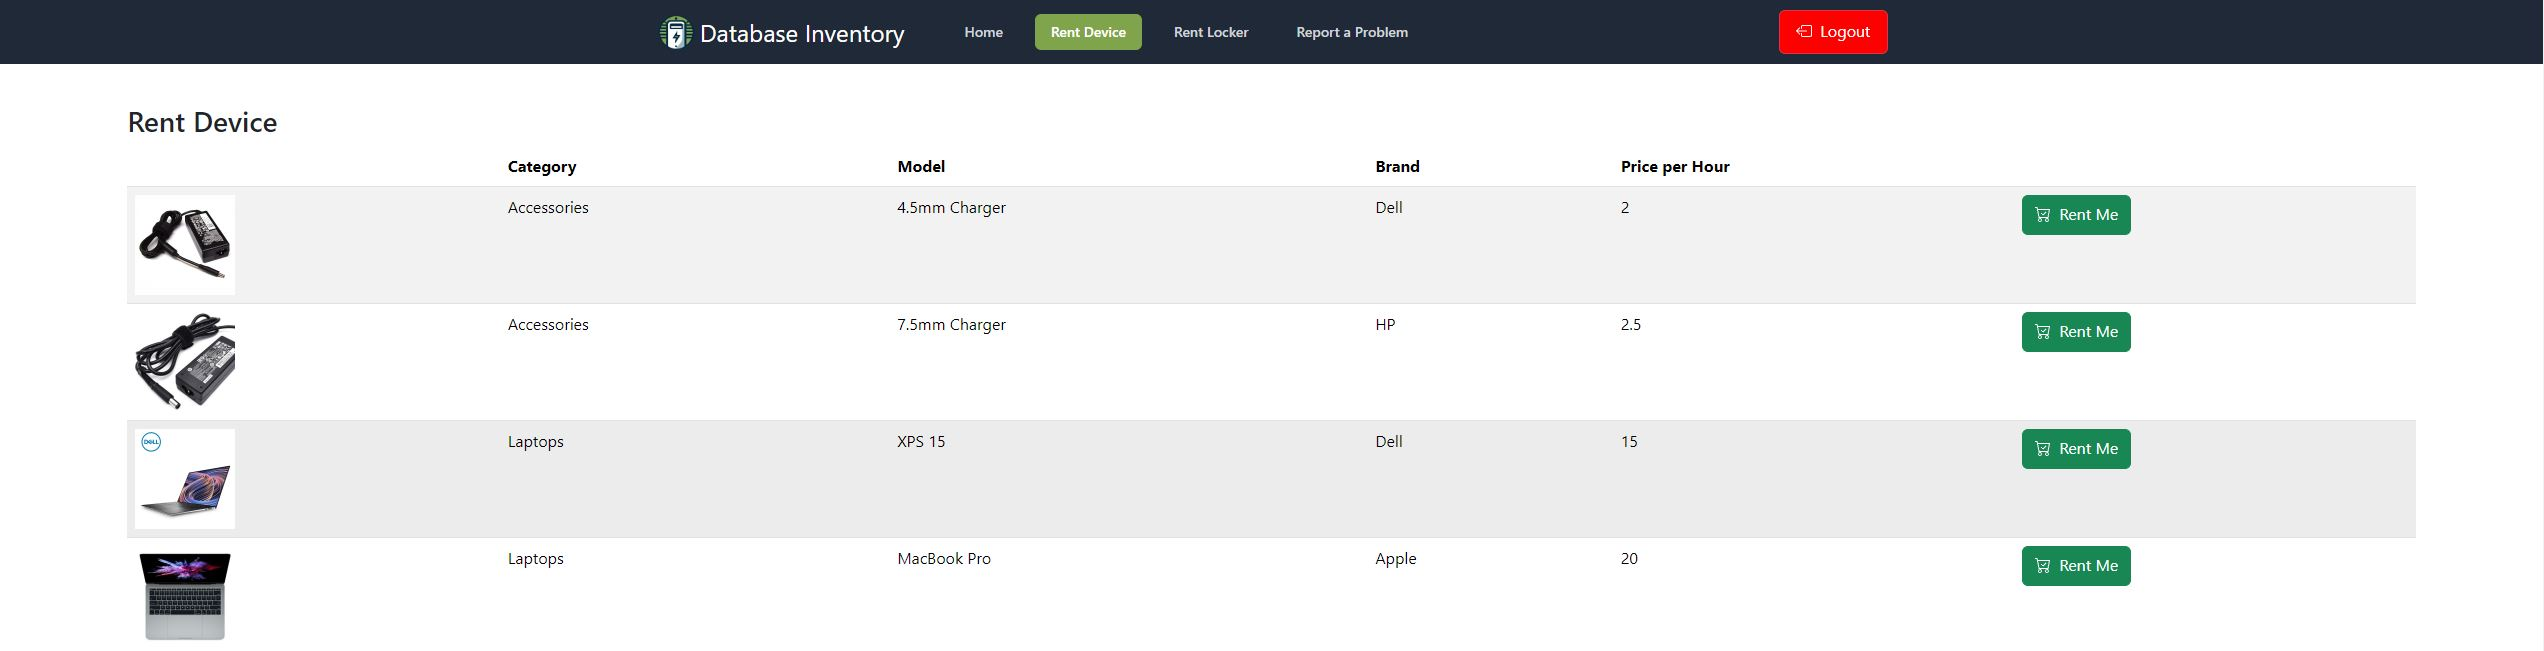
\includegraphics[width=1\linewidth]{images/rent device.JPG}
    \caption{User Frontend Rent Device}
    \label{fig:rent-device-dashboard}
\end{figure}
\newpage
\item \textbf{User Frontend Rent Device Confirmation:} In this confirmation modal, users receive a pin code to access the locker. Additionally, the modal includes a Google Map showing the location of the device or locker, enhancing user convenience and security.
\begin{figure}[h]
    \centering
    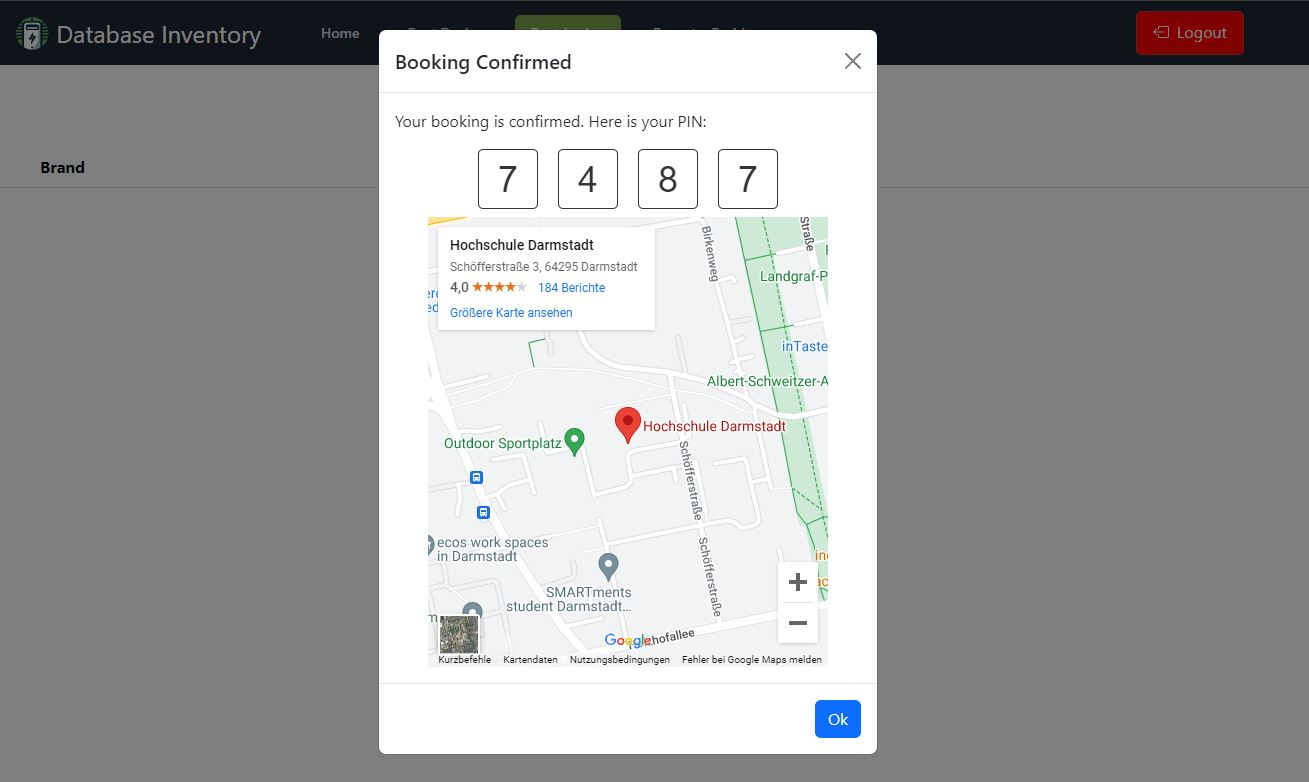
\includegraphics[width=1\linewidth]{images/booking conf.JPG}
    \caption{User Frontend Rent Device Confirmation}
    \label{fig:rent-device-confirmation-modal}
\end{figure}

\item \textbf{User Frontend Locker Wattage Overview:} This view provides users with real-time information on whether the device is currently charging. If the wattage flow is off, it indicates that the device is fully charged, offering users insight into the device's charging status.
\begin{figure}[h]
    \centering
    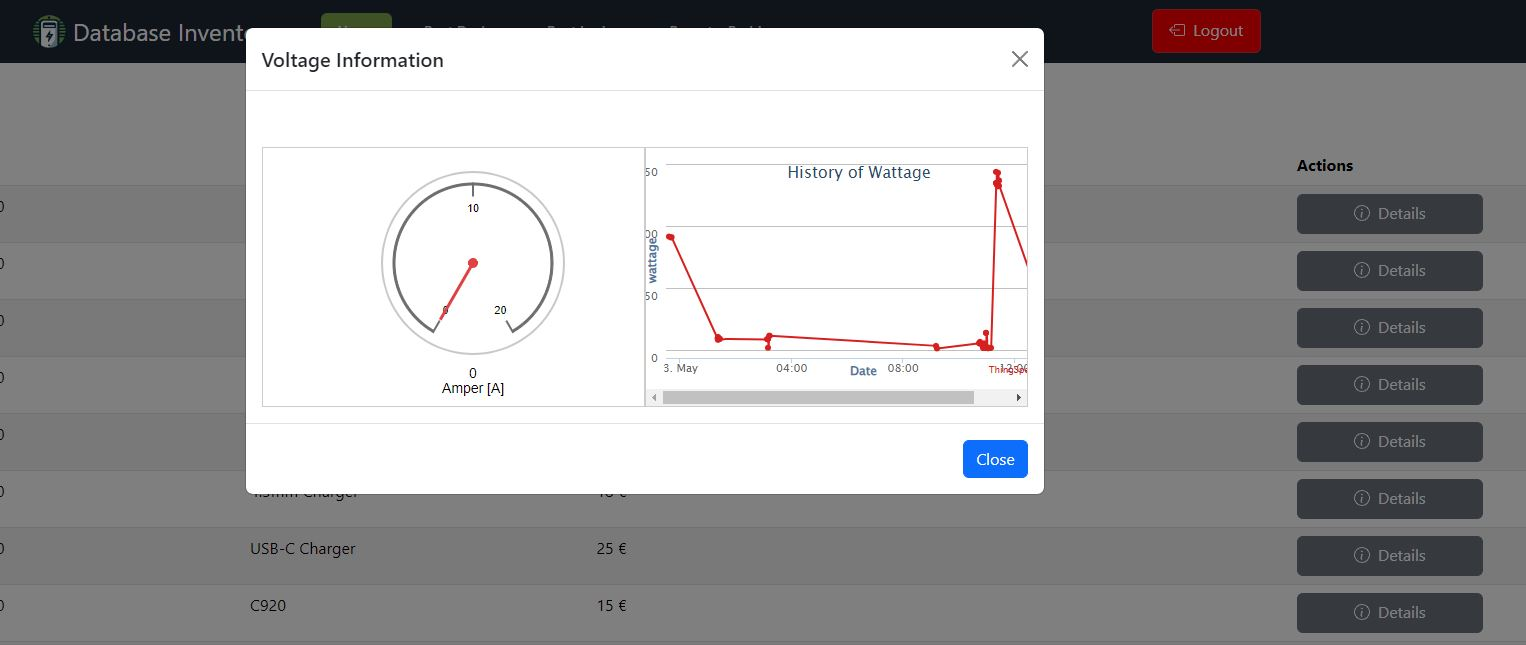
\includegraphics[width=1\linewidth]{images/user_wattage.JPG}
    \caption{User Frontend Locker Wattage Overview}
    \label{fig:locker-wattage-overview}
\end{figure}
\end{itemize}


\subsection{Backend}
{\tiny Written by: Sven Lepper}\\

\subsection{Backend Implementation} \label{sec:Implementation_Backend}

This subsection provides an overview of the implementation details for the backend of the locker system. It covers the technologies, frameworks, and development environment used in the development process.

\subsubsection{Project Setup}

The backend part of the locker system project is developed using FastAPI and SQLAlchemy/alembic. These technologies were chosen for their robustness, scalability, and ease of use in building web APIs and managing database migrations.

The development environment setup involves several steps to ensure a smooth workflow. Firstly, it requires a local Postgres database instance to be running, with specific configuration settings provided via environment variables. These variables include the database username, password, host, port, and name.

The project setup also involves cloning the backend repository and configuring the environment variables as necessary. A virtual environment is then created to isolate dependencies, followed by the installation of required packages specified in the `requirements.txt` file using pip.

Once the development environment is set up, the application can be run locally by activating the virtual environment and starting the application. Additionally, database migrations can be managed using alembic, with commands provided to generate and apply migration scripts.

\subsubsection{List of Important Libraries and Versions}

The following list includes the most important libraries used in the backend implementation along with their versions:

\begin{itemize}
    \item \textbf{\href{https://fastapi.tiangolo.com/}{FastAPI}} (\texttt{fastapi==0.110.2}): FastAPI is a modern, fast (high-performance) web framework for building APIs with Python 3.7+ based on standard Python type hints.

    \item \textbf{\href{https://www.sqlalchemy.org/}{SQLAlchemy}} (\texttt{SQLAlchemy==2.0.29}): SQLAlchemy is the Python SQL toolkit and Object-Relational Mapper that gives application developers the full power and flexibility of SQL.

    \item \textbf{\href{https://alembic.sqlalchemy.org/en/latest/}{Alembic}} (\texttt{alembic==1.13.1}): Alembic is a lightweight database migration tool for usage with the SQLAlchemy Database Toolkit for Python.

    \item \textbf{\href{https://docs.pydantic.dev/latest/}{Pydantic}} (\texttt{pydantic==2.7.1}): Pydantic is a data validation and settings management using Python type annotations.

    \item \textbf{\href{https://www.uvicorn.org/}{uvicorn}} (\texttt{uvicorn==0.29.0}): Uvicorn is a lightning-fast ASGI server implementation, using uvloop and httptools.

    \item \textbf{\href{https://pypi.org/project/psycopg2/}{Psycopg2}}: Psycopg is the most popular PostgreSQL database adapter for the Python programming language.
\end{itemize}

\subsubsection{Request Handling in FastAPI and SQLAlchemy}

A crucial aspect of understanding the backend implementation is to grasp how FastAPI and SQLAlchemy handle incoming requests and interact with the database. The following diagram illustrates the request handling process:

\begin{figure}[h]
    \centering
    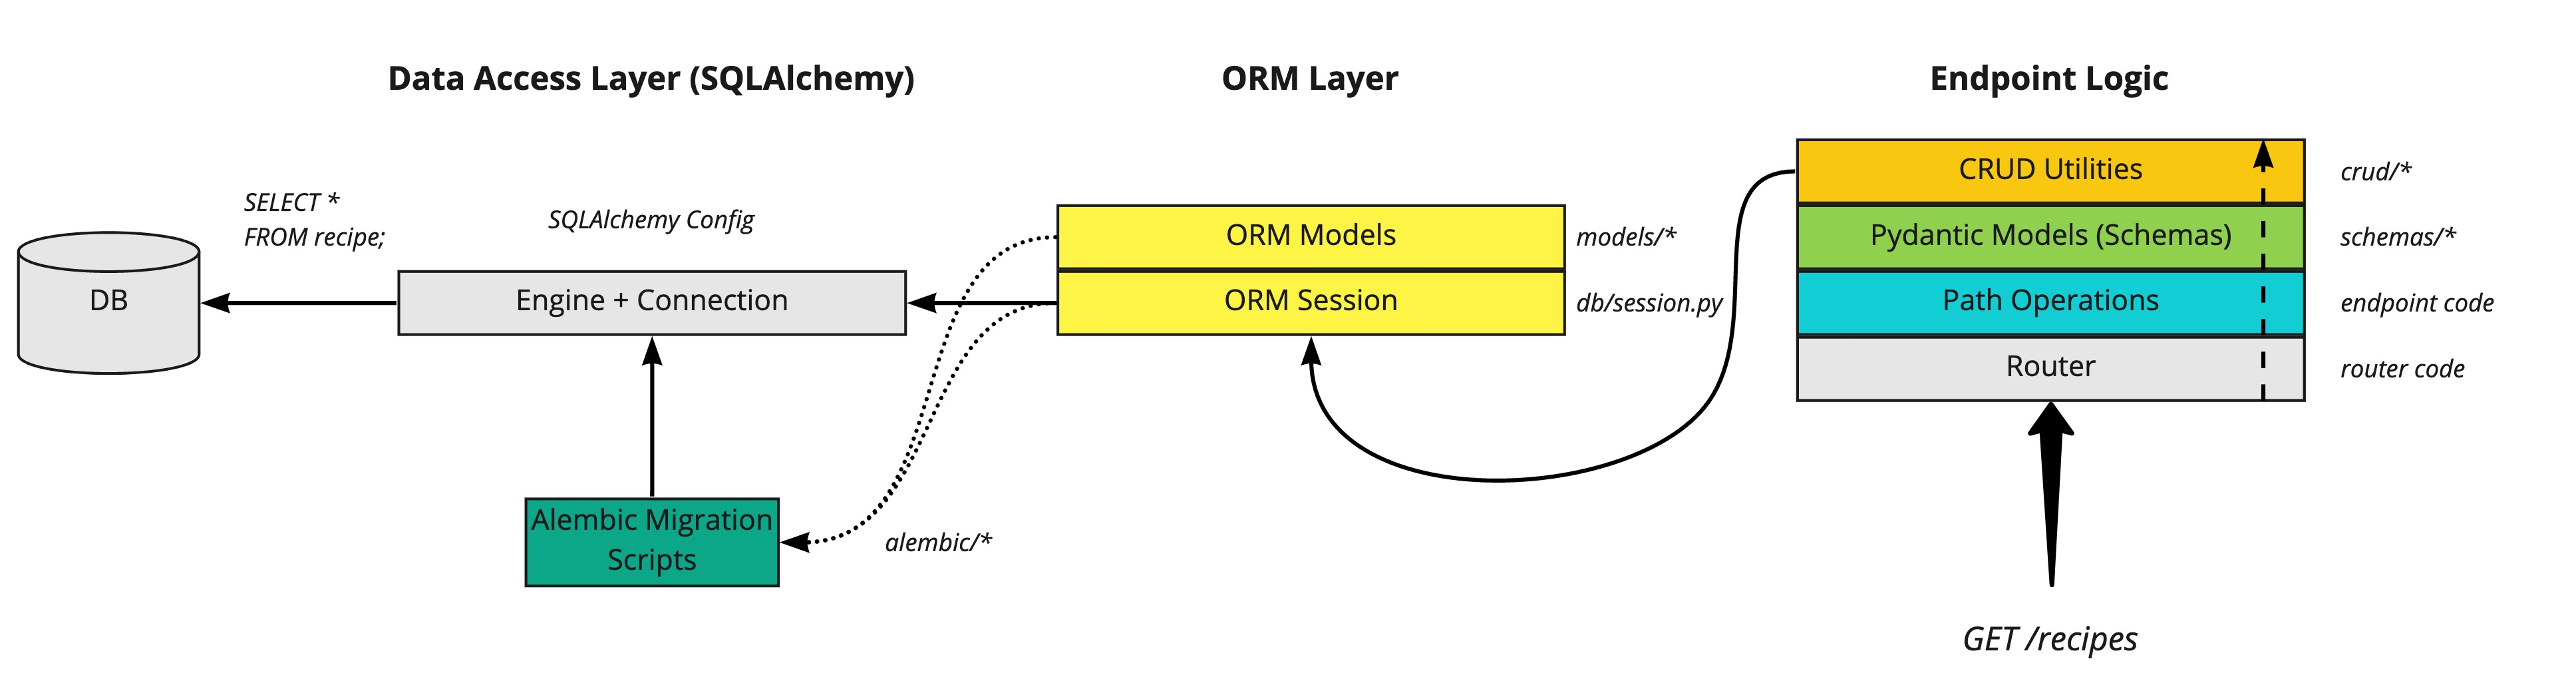
\includegraphics[width=0.8\textwidth]{images/request_handling_diagram}
    \caption{Request Handling in FastAPI and SQLAlchemy \cite{samiullah_fastapi_tutorial}}
    \label{fig:request_handling}
\end{figure}


This diagram visually represents the sequence of steps involved in processing a client request, starting from the client making an HTTP request to the backend API. FastAPI routes the request to the appropriate endpoint, where it is processed by the corresponding router function. The router function interacts with the database through SQLAlchemy ORM, executing CRUD operations as necessary to fulfill the request. Once the database operations are complete, a response is generated and returned to the client.

Understanding this request handling flow is essential for developers to comprehend the inner workings of the backend system and troubleshoot any issues that may arise during development or deployment.


\subsubsection{Project Structure}

The backend part of the locker system project adheres to a well-organized structure, following best practices to ensure clarity, modularity, and maintainability. Below is an overview of the project structure and the rationale behind each component:

\begin{itemize}
    \item \textbf{README.md}: This file serves as the project's main documentation hub, containing comprehensive information on setup instructions, deployment steps, and other essential details. A well-written README enhances project understanding and facilitates collaboration among team members.

    \item \textbf{requirements.txt}: This file enumerates all Python packages required by the project, making it easy for developers to install dependencies using pip. Managing dependencies in a centralized file promotes consistency and reproducibility across different environments.

    \item \textbf{.env}: Environment variables play a crucial role in configuring the application, especially sensitive information like database credentials. Utilizing a separate .env file allows for easy management of configuration settings across various deployment environments.

    \item \textbf{venv}: The virtual environment isolates project dependencies, ensuring compatibility and preventing conflicts with other Python projects. By encapsulating dependencies within a dedicated environment, developers can maintain a clean and reproducible development setup.

    \item \textbf{alembic/versions}: This directory houses database migration files managed by Alembic, a lightweight migration tool for SQLAlchemy. Organizing migrations in a structured manner facilitates version control and systematic evolution of the database schema over time.

    \item \textbf{images}: Images used in the project documentation, such as the README file, are stored in this directory. Including visuals enhances readability and comprehension of project-related instructions and guidelines.

    \item \textbf{Dockerfile}: Docker simplifies application deployment by encapsulating the application and its dependencies into portable containers. The Dockerfile specifies the steps to build a Docker image, promoting consistency and reproducibility across different deployment environments.
\end{itemize}

The \textbf{app} folder encapsulates the core components of the backend application. It is further divided into the following subdirectories and files (examples are used from the Category class, but the structure is the same for all classes):

\begin{itemize}
    \item \textbf{api} folder: This folder contains endpoint-specific modules responsible for handling HTTP requests and responses. Each endpoint module typically consists of three main components:

    \begin{itemize}
        \item \textbf{CRUD operations (Create, Read, Update, Delete)}: These operations define the basic functionalities for interacting with database entities. For example, the \texttt{crud.py} files contain functions for creating, retrieving, updating, and deleting records from the database.

        The following code snippet demonstrates the \texttt{delete\_category\_by\_id} function, which is responsible for deleting a category from the database by its ID:

        \begin{lstlisting}[language=Python]
        def delete_category_by_id(category_id: int, db: Session):
            category = get_category_by_id(category_id, db)
            if category:
                db.delete(category)
                db.commit()
        \end{lstlisting}

        This function first retrieves the category with the specified ID using the \texttt{get\_category\_by\_id} function. If the category exists, it is deleted from the database using the SQLAlchemy \texttt{delete} method, followed by a commit to persist the changes.


        \item \textbf{Router functions}: The \texttt{router.py} files define FastAPI router instances responsible for routing HTTP requests to the appropriate endpoint functions. Routers enhance code organization and modularity by grouping related endpoint operations together.

        The following code snippet illustrates a router function responsible for handling HTTP DELETE requests to delete a category:

        \begin{lstlisting}[language=Python]
        @router.delete('/categories/{category_id}', response_model=None, tags=['category'])
        def delete_category(
                category_id: int,
                db: Session = Depends(get_db)):
            category_crud.delete_category_by_id(category_id, db)
            return Response(status_code=status.HTTP_204_NO_CONTENT)
        \end{lstlisting}

        In this function, the route decorator specifies the HTTP method (DELETE) and the endpoint URL pattern ("/categories/{category\_id}"). The function parameters include the category ID to be deleted and a database session dependency obtained through the \texttt{get\_db} function. Inside the function, the \texttt{delete\_category\_by\_id} function from the CRUD module (\texttt{category\_crud}) is called to delete the category from the database. Finally, a 204 No Content response is returned to indicate successful deletion.


        \item \textbf{Schema definitions}: Schemas define the structure and validation rules for request and response payloads exchanged between the client and server. The \texttt{schemas.py} files contain Pydantic models representing data schemas for serialization and validation purposes.

        The following code snippet presents a Pydantic model (\texttt{CategoryBaseSchema}) defined in a schema file:

        \begin{lstlisting}[language=Python]
        class CategoryBaseSchema(BaseModel):
            name: str
        \end{lstlisting}

        In this schema definition, \texttt{CategoryBaseSchema} inherits from \texttt{BaseModel}, a Pydantic base class used for defining data models. The schema consists of a single field (\texttt{name}) with a data type of \texttt{str}, representing the name of a category. Pydantic models provide automatic data validation based on the specified field types, enabling robust input validation and serialization/deserialization of data between client and server components.

    \end{itemize}

    \item \textbf{db} folder: This folder contains modules related to database management and configuration. Key components include:

    \begin{itemize}
        \item \textbf{Configuration module (\texttt{config.py})}: This module defines database connection settings using environment variables and provides functions for establishing database connections and checking connectivity status. Centralizing database configuration facilitates easy maintenance and deployment across different environments.

        The following code snippet illustrates the \texttt{config.py} module, which manages database configuration:

        \begin{lstlisting}[language=Python]
        from sqlalchemy import create_engine
        from sqlalchemy.orm import sessionmaker
        from sqlalchemy.exc import OperationalError
        from dotenv import load_dotenv
        import os

        load_dotenv()

        DB_USERNAME = os.getenv("DATABASE_USERNAME")
        DB_PASSWORD = os.getenv("DATABASE_PASSWORD")
        DB_HOST = os.getenv("DATABASE_HOST")
        DB_PORT = os.getenv("DATABASE_PORT")
        DB_NAME = os.getenv("DATABASE_NAME")
        DB_URL = f"postgresql://{DB_USERNAME}:{DB_PASSWORD}@{DB_HOST}:{DB_PORT}/{DB_NAME}"

        def get_database_url():
            return DB_URL

        engine = create_engine(DB_URL)
        SessionLocal = sessionmaker(autocommit=False, autoflush=False, bind=engine)

        def check_database_connection():
            try:
                engine = create_engine(DB_URL)
                with engine.connect():
                    return True
            except OperationalError:
                return False
        \end{lstlisting}

        This module loads database connection settings from environment variables using the \texttt{dotenv} library. It defines functions for retrieving the database URL, establishing a database engine, and checking database connectivity. By encapsulating database configuration in a single module, the codebase becomes more modular and maintainable, enabling seamless deployment across various environments.


        \item \textbf{Model definitions (\texttt{models.py})}: Models define the structure of database tables and their relationships using SQLAlchemy declarative base. Models encapsulate business logic and data integrity constraints, promoting code organization and reusability.

        The following code snippet demonstrates a model definition (\texttt{Category}) in the \texttt{models.py} module:

        \begin{lstlisting}[language=Python]
        from sqlalchemy import Column, Integer, String
        from db.config import Base

        class Category(Base):
            __tablename__ = 'categories'

            id = Column(Integer, primary_key=True)
            name = Column(String, nullable=False)
        \end{lstlisting}

        In this model definition, \texttt{Category} is a SQLAlchemy model representing the \texttt{categories} table in the database. It inherits from \texttt{Base}, the declarative base provided by SQLAlchemy. The \texttt{\_\_tablename\_\_} attribute specifies the table name, while \texttt{id} and \texttt{name} represent the table columns. By encapsulating database schema in model classes, the codebase becomes more organized and maintainable, facilitating data manipulation and ensuring data integrity.
    \end{itemize}

    \item \textbf{main.py}: The main entry point of the backend application, responsible for initializing the FastAPI application instance and configuring middleware, routers, and other application-level settings.
\end{itemize}

\subsubsection{API Design}

The backend API is documented using the OpenAPI Specification (OAS) format, commonly known as Swagger. Swagger provides a standardized, machine-readable representation of the API, detailing its endpoints, request/response formats, and data models.

\textbf{What is Swagger?}:
Swagger is an open-source framework that enables the design, documentation, and testing of RESTful APIs. It defines a structured format for describing API endpoints, parameters, responses, and authentication mechanisms, facilitating seamless integration and collaboration among developers.

\begin{figure}[h]
    \centering
    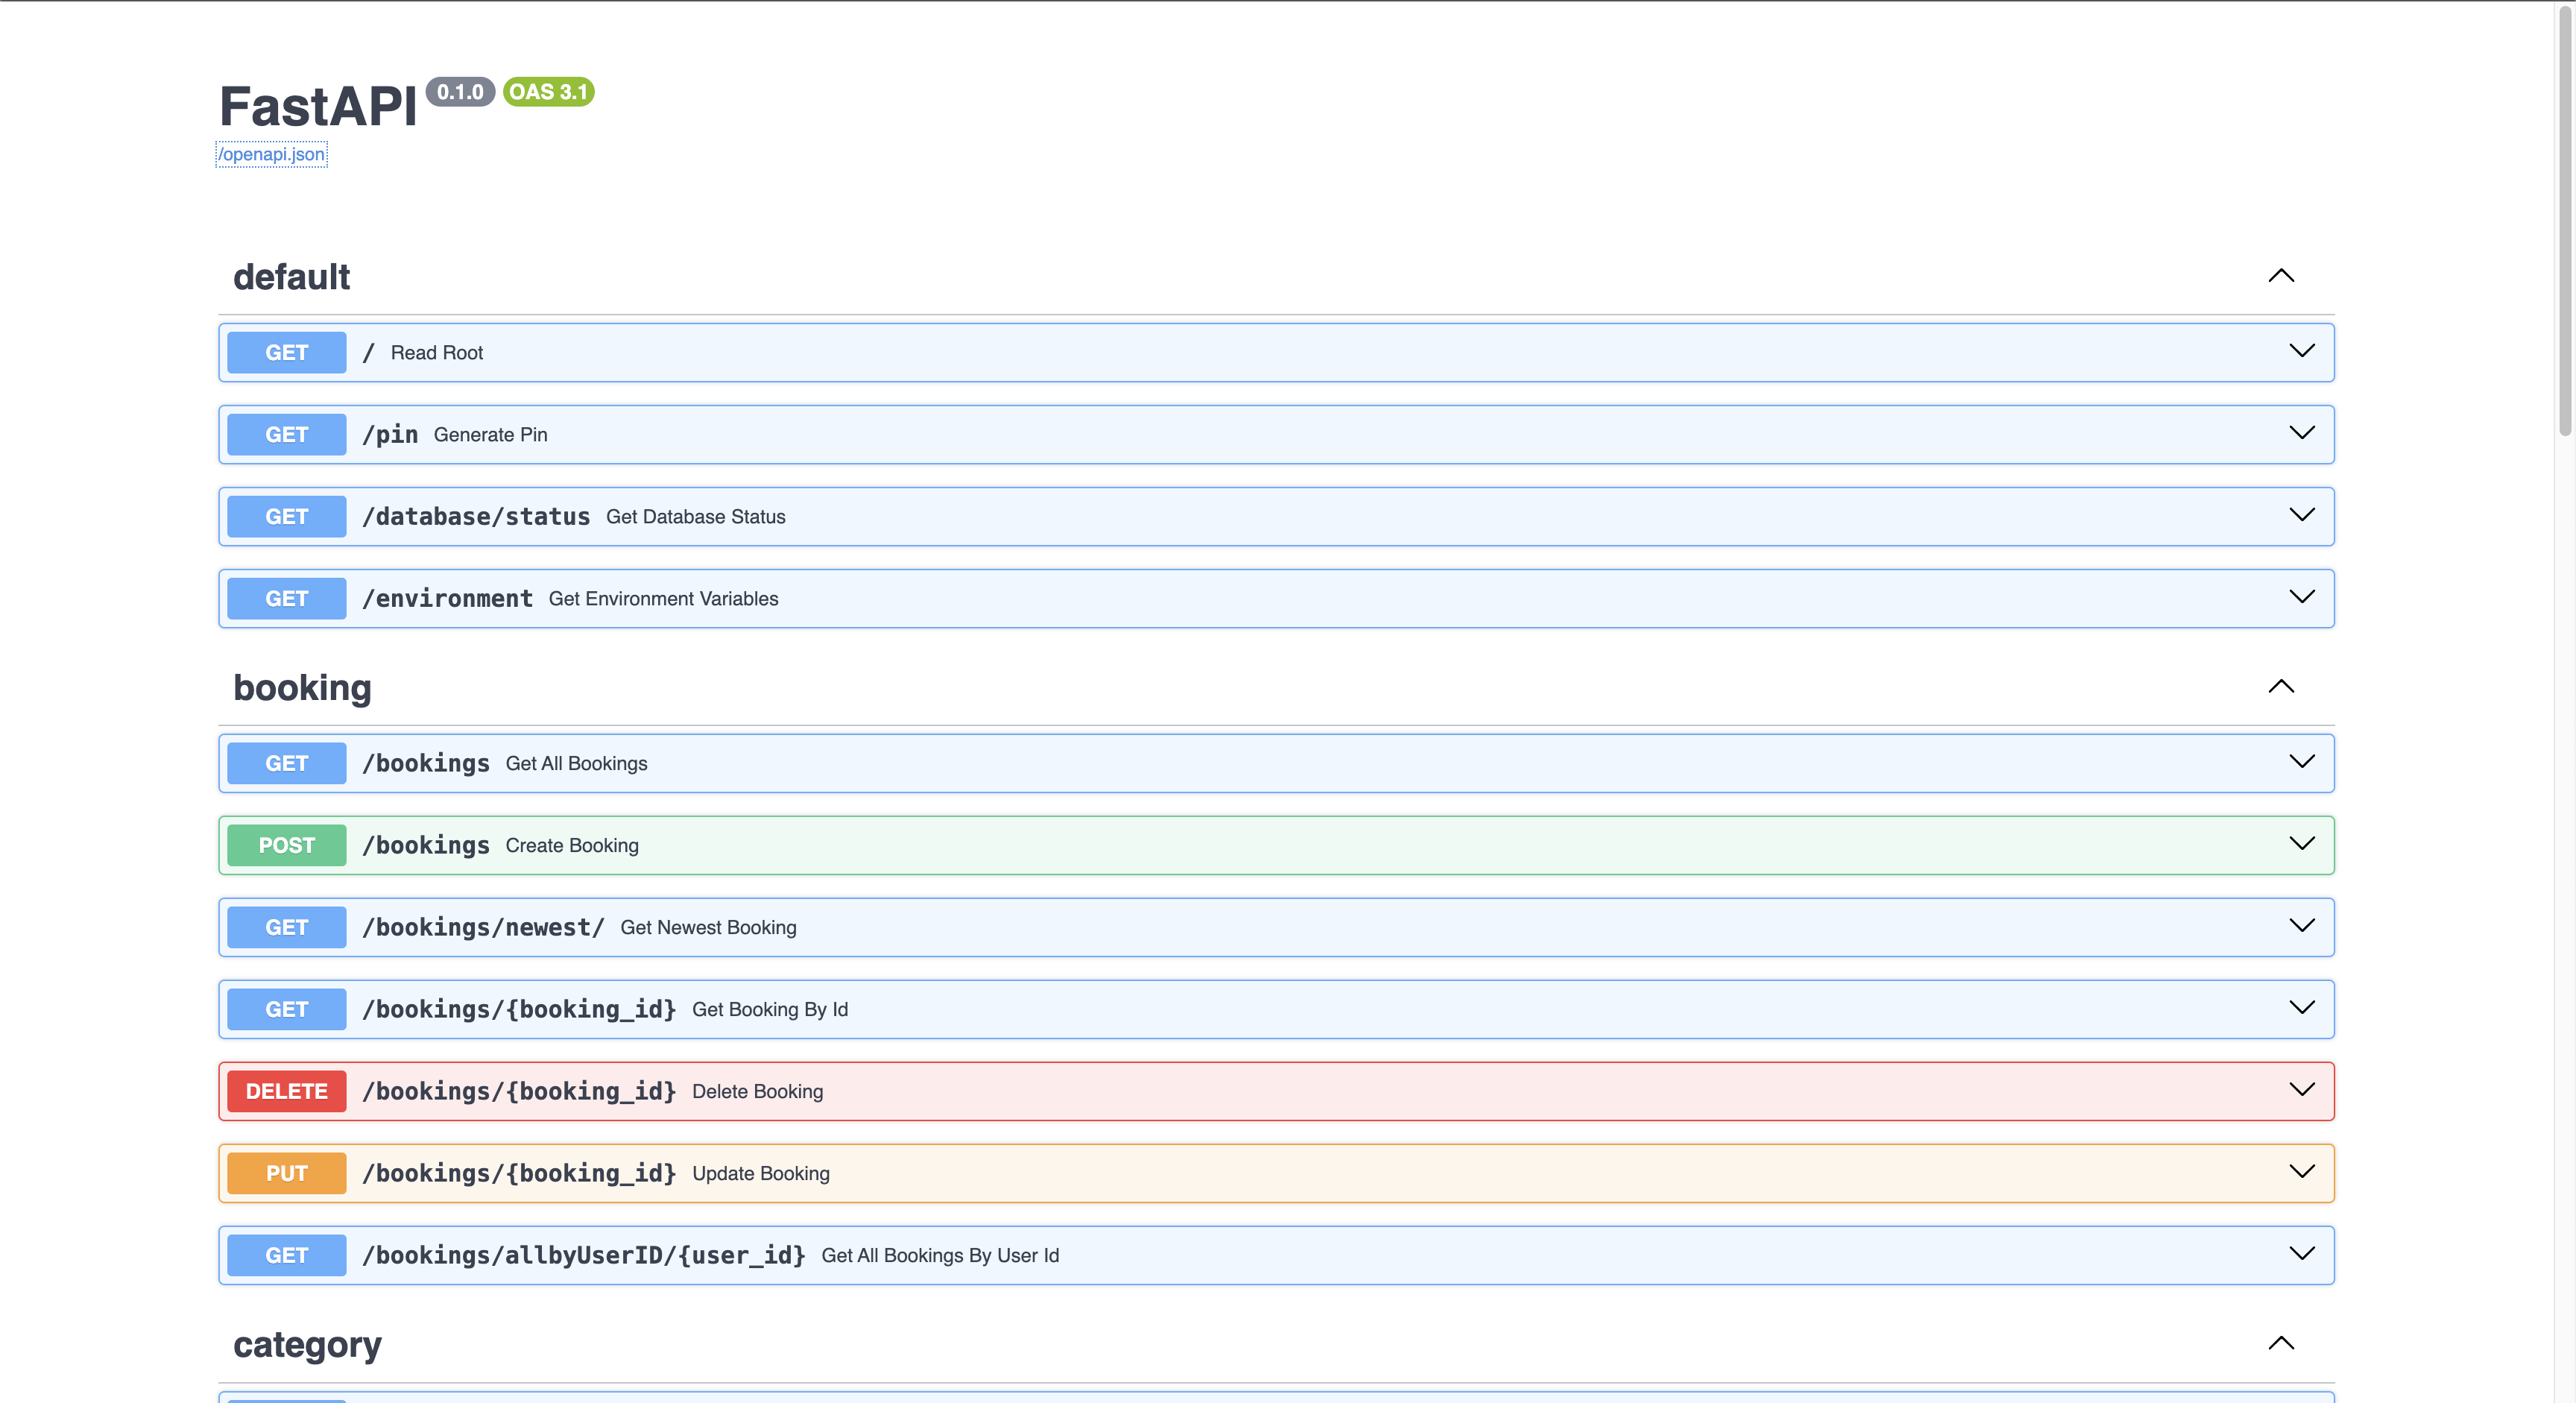
\includegraphics[width=0.8\textwidth]{images/swagger_ui}
    \caption{FastAPI Swagger UI}
    \label{fig:swagger_ui}
\end{figure}

\textbf{Why is Swagger Useful?}:
Swagger simplifies API development by offering a centralized platform for describing and visualizing API specifications. It enhances communication between frontend and backend developers, accelerates client-side integration, and fosters interoperability across diverse programming languages and frameworks.

\textbf{FastAPI and Swagger}:
FastAPI, a modern web framework for building APIs with Python, integrates seamlessly with Swagger to automate API documentation. FastAPI generates Swagger UI out of the box, allowing developers to interactively explore and test API endpoints. By leveraging FastAPI's native support for Swagger, developers can focus on implementing business logic without worrying about manual documentation efforts.

\textbf{Endpoints Definition}:
The backend API comprises a set of well-defined endpoints, each catering to a specific functionality within the locker system. Endpoints such as \texttt{/bookings}, \texttt{/categories}, \texttt{/devices}, \texttt{/reports}, \texttt{/users}, among others, provide access to the corresponding resources and operations.

\begin{figure}[h]
    \centering
    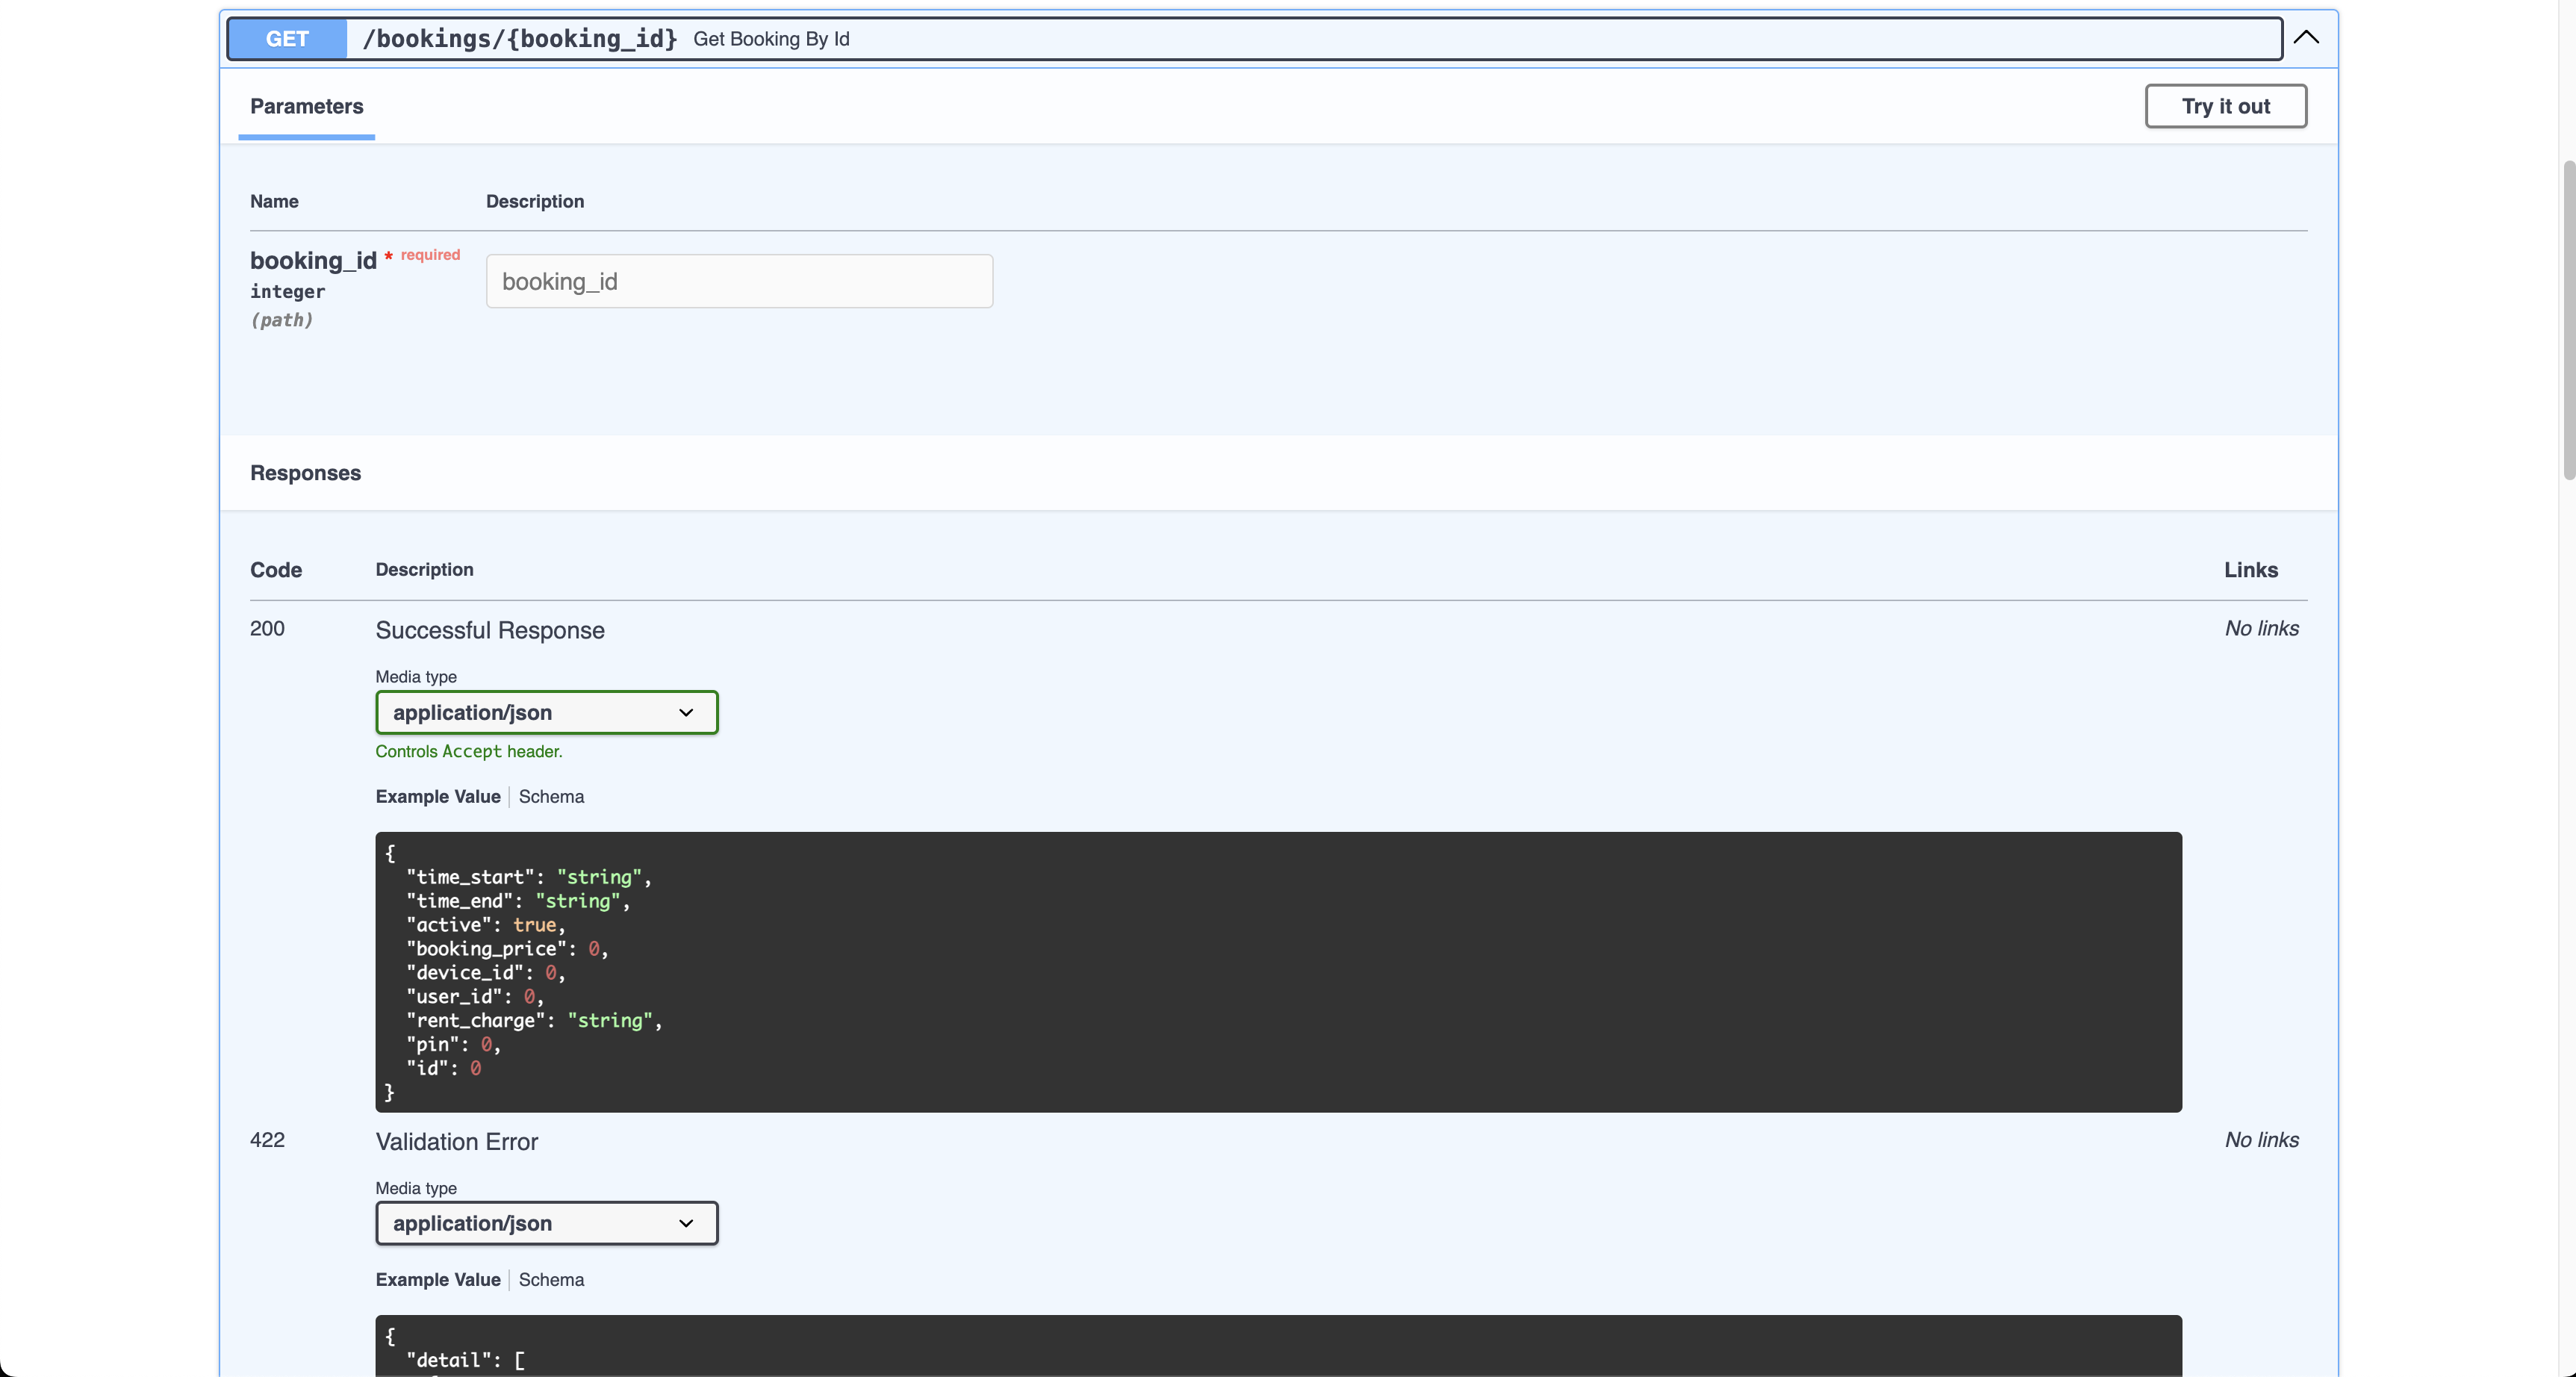
\includegraphics[width=0.8\textwidth]{images/swagger_ui_bookings}
    \caption{FastAPI Swagger UI - Bookings Endpoint}
    \label{fig:swagger_ui_bookings}
\end{figure}

\textbf{Request/Response Formats}:
For each endpoint, clear specifications are provided regarding the expected request formats, including request bodies, query parameters, and path parameters. Similarly, the response formats, denoted by response schemas, outline the structure of data returned by the server in response to client requests.

\textbf{Data Models}:
The API leverages distinct data models to represent various entities and their attributes. These models, including \texttt{BookingSchema}, \texttt{CategorySchema}, \texttt{DeviceSchema}, \texttt{ReportSchema}, and \texttt{UserSchema}, encapsulate the structure of data exchanged between the client and server. Additionally, specialized schemas such as \texttt{BookingCreateSchema}, \texttt{CategoryCreateSchema}, and others are utilized for specific operations, ensuring consistency and validation of incoming data.

\subsubsection{Database Schema Design}

The database schema for the locker system is designed to efficiently store information related to bookings, categories, devices, reports, and users. The schema employs normalization techniques to minimize redundancy and ensure data integrity. Indexing strategies are implemented to optimize query performance, particularly for frequently accessed fields.

\begin{figure}[h]
    \centering
    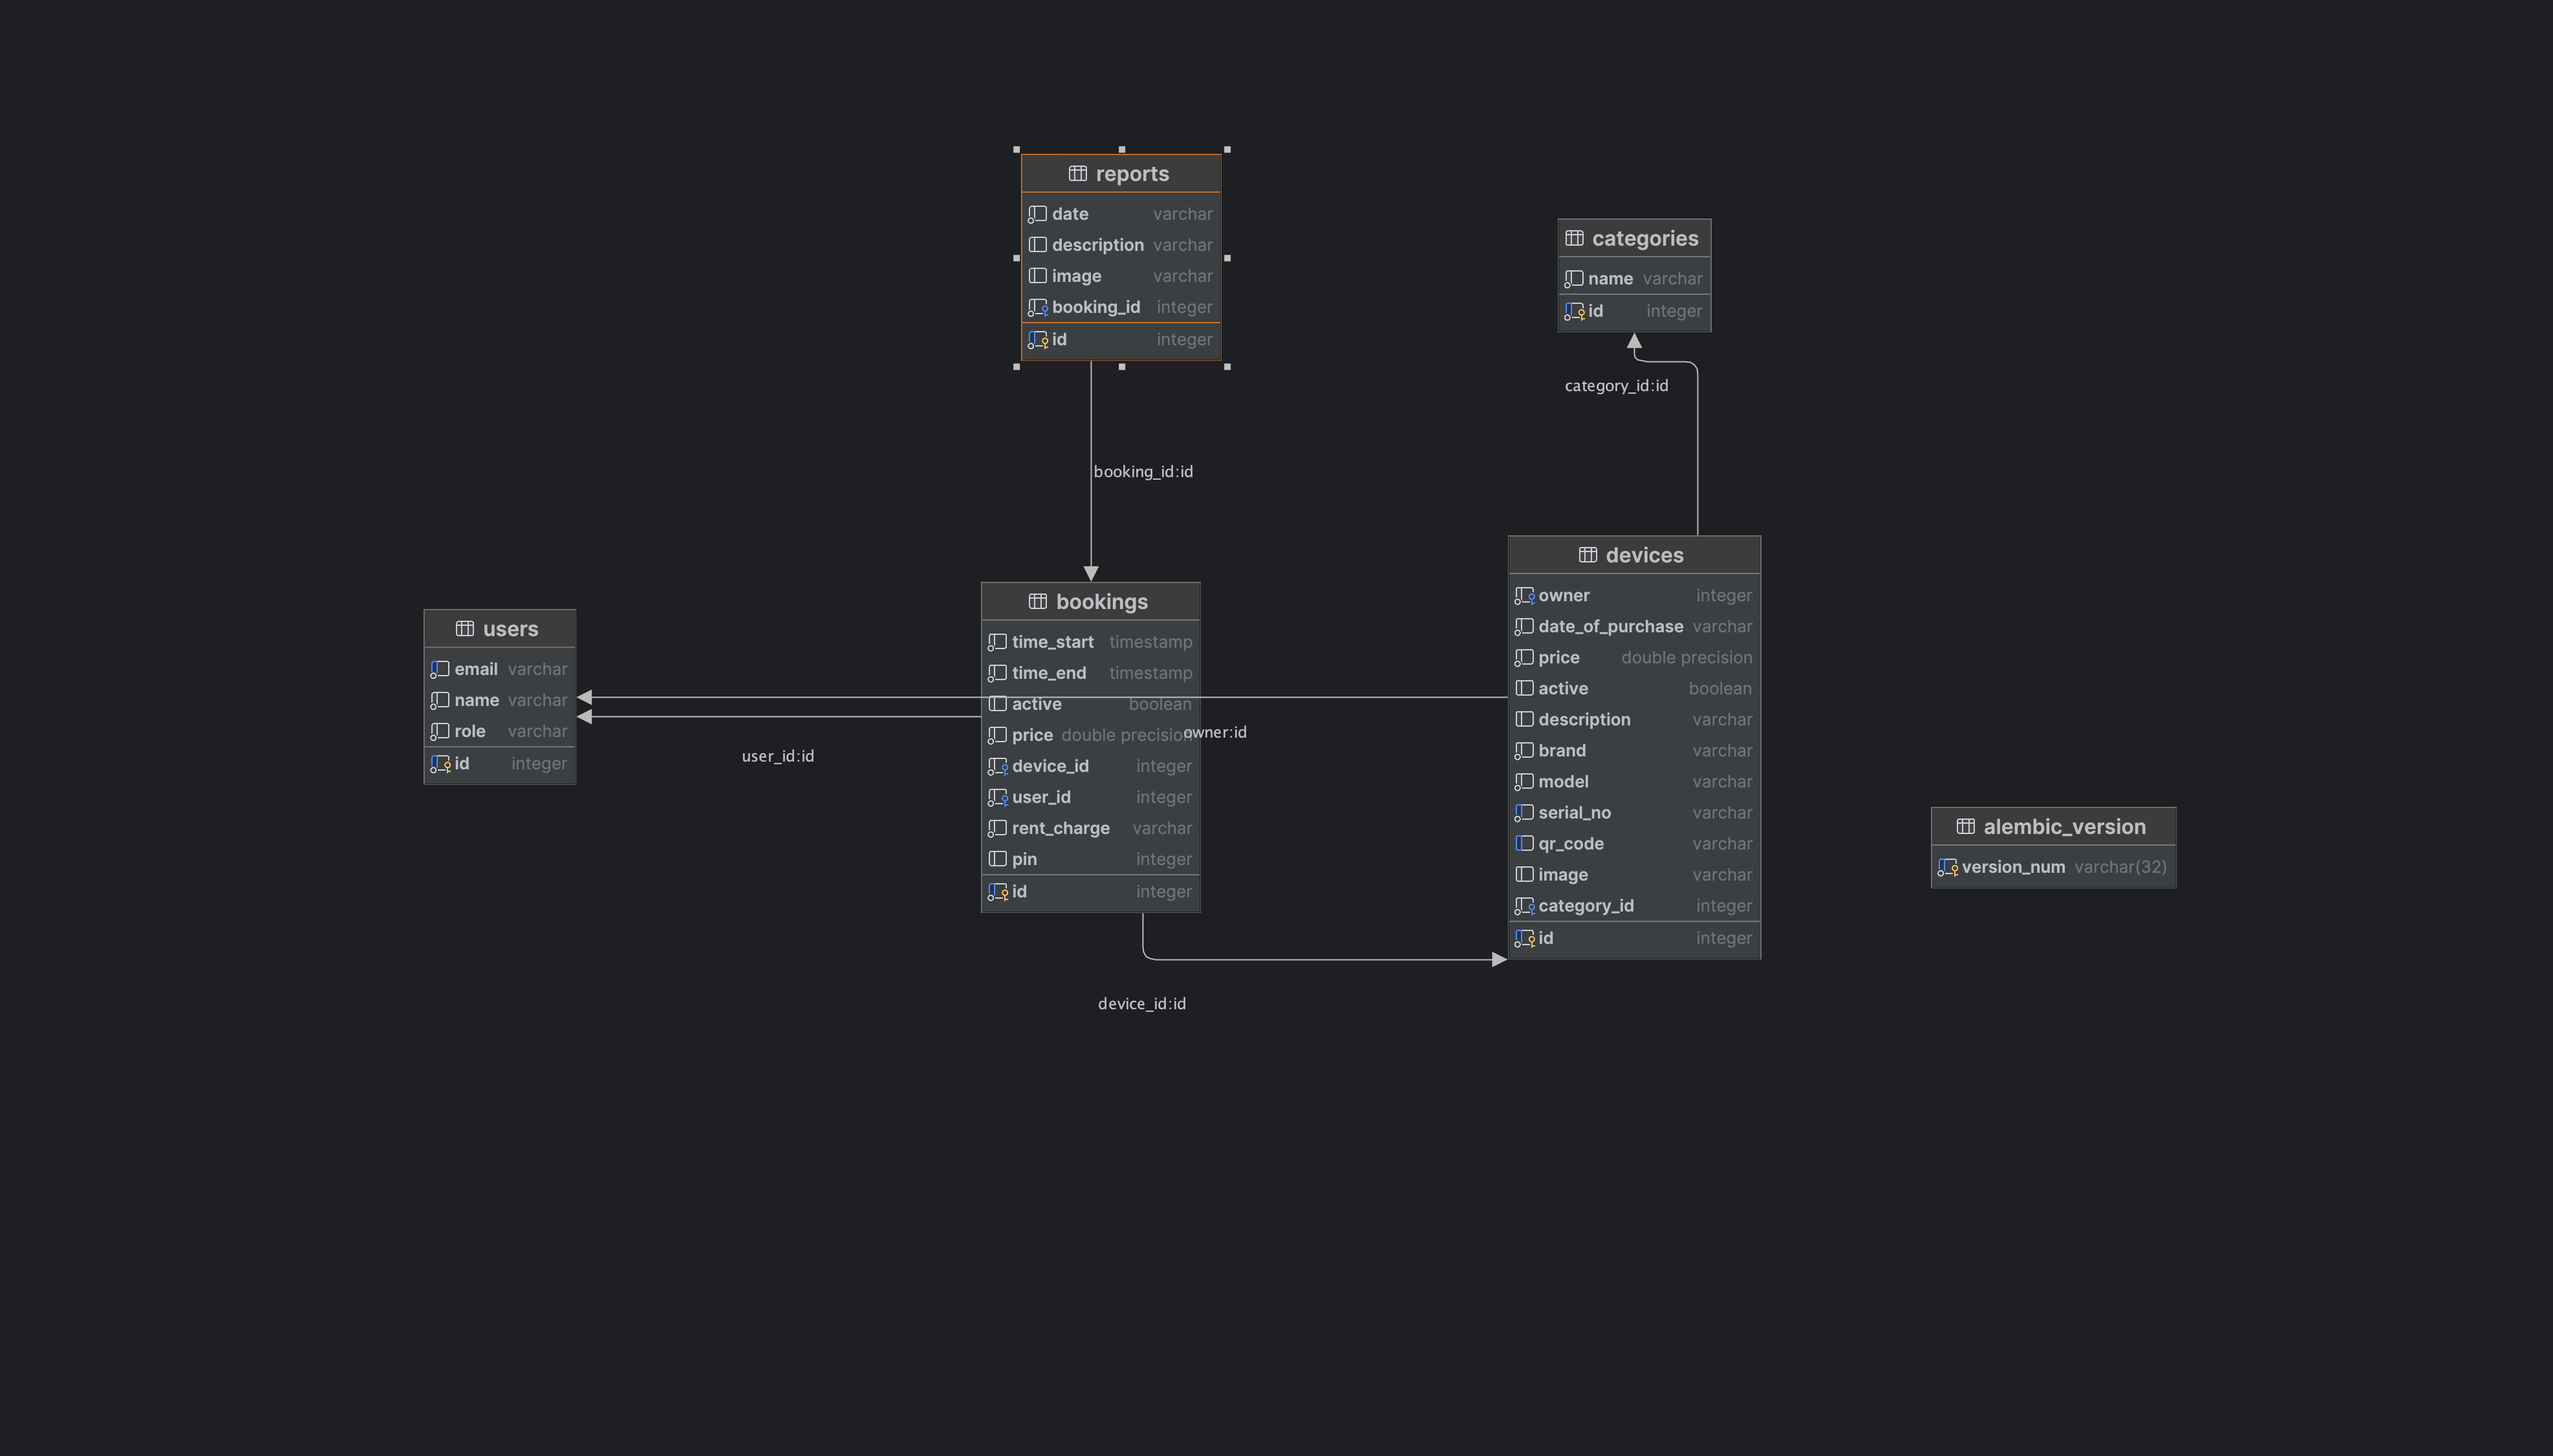
\includegraphics[width=0.8\textwidth]{images/db_schema}
    \caption{Database Schema Design}
    \label{fig:dbschema}
\end{figure}

\textbf{Normalization}:
The schema adheres to normalization principles to eliminate data redundancy and dependency issues. By organizing data into well-structured tables and establishing relationships between them, normalization ensures efficient data storage and maintenance.

\textbf{Indexing}:
To enhance query performance, the database schema incorporates appropriate indexes on key fields. Indexing accelerates data retrieval operations by facilitating quick access to specific records, especially in scenarios involving large datasets.

\textbf{Optimization}:
The schema design incorporates optimization strategies to streamline database operations and enhance overall system performance. Techniques such as query optimization, caching, and resource allocation are employed to mitigate bottlenecks and ensure optimal resource utilization.

\subsubsection{Logging}

Logging plays a crucial role in monitoring and troubleshooting the backend operations of the locker system. By capturing relevant information during runtime, logging enables developers to track system behavior, identify errors, and analyze performance metrics.

\textbf{Logging Implementation}:
The backend API incorporates logging functionality to record significant events and activities. The Python logging module provides a flexible framework for logging messages of varying severity levels to different destinations, including files, streams, or external services.

\textbf{Example:} Consider the following function for creating a booking within the locker system:

\begin{lstlisting}[language=Python]
def create_booking(schema: BookingCreateSchema, db: Session):
    entity = Booking(**schema.dict())
    entity.pin = random.randint(1000, 9999)
    logging.info('Booking created with id {}'.format(entity.id))
    db.add(entity)
    db.commit()
    return entity
\end{lstlisting}

In this example, the \texttt{create\_booking} function creates a new booking entity based on the provided schema. After generating a random PIN for the booking, the function logs a message indicating the successful creation of the booking along with its ID. This logging statement provides valuable insights into the system's activity and facilitates debugging and auditing processes.

\subsubsection{Areas for Improvement}

While the backend implementation of the locker system prototype adheres to common best practices, several areas require further attention and refinement before the system can be considered production-ready:

\begin{itemize}
    \item \textbf{Error Handling}: The current implementation lacks comprehensive error handling mechanisms, which are essential for gracefully managing unexpected scenarios and providing informative feedback to users. For example, enhancing error responses with appropriate status codes and error messages would improve the system's robustness.

    \item \textbf{Infrastructure}: The prototype operates in a development environment and lacks the infrastructure necessary for deployment in a production setting. Implementing scalable infrastructure components, such as load balancers, auto-scaling groups, and fault-tolerant databases, is crucial for ensuring system reliability and performance under varying workloads.

    \item \textbf{Validation}: While basic input validation is incorporated into the API endpoints, there is room for strengthening validation logic to enforce data integrity and prevent malicious inputs. Implementing robust validation mechanisms, such as input sanitization and parameter validation, would enhance the security and reliability of the system.

    \item \textbf{Security}: Security measures, including authentication, authorization, and data encryption, are fundamental requirements for safeguarding sensitive information and protecting the system against security threats. Implementing authentication mechanisms, role-based access control (RBAC), and encryption protocols would mitigate security risks and enhance the system's trustworthiness.
\end{itemize}

Addressing these areas of improvement would contribute to the development of a robust, secure, and scalable backend system for the locker application.



\subsection{Arduino}
{\tiny Written by: Felix}

\subsection{Arduino Implementation}

\subsubsection{Arduino Setup}

The Arduino component of the locker system project is developed using Arduino IDE version 2.3.2 \cite{arduino-software}. This development environment ensures a streamlined workflow, particularly when the Arduino is connected via USB, with logs displayed within the IDE's Terminal.

To set up the Arduino for this project, follow these steps:

\begin{enumerate}
    \item \textbf{Cloning the Arduino Repository}:
    Begin by cloning the Arduino repository referenced in the project documentation \cite{inventory-database-arduino}.
    
    \item \textbf{Wiring the Cables}:
    Refer to the Fritzing diagram provided in Section \ref{sec:ArduinoFritzing} Figure \ref*{fig:ardFritzing} to correctly wire the components for the Arduino setup.
    
    \item \textbf{Downloading Required Libraries}:
    Utilize the Arduino IDE specified in Section \ref{sec:ArduinoLibaries} to download and integrate the necessary libraries into your project.
    
    \item \textbf{Configuring WiFi Connection}:
    Update the WiFi credentials within the Arduino sketch as illustrated below:
    
    \begin{lstlisting}[language=C++, caption={WiFi Configuration in Arduino Sketch}]
    // WiFi Configuration
    #include <WiFiNINA.h>
    char ssid[] = "YOUR_SSID";
    char wifi_password[] = "YOUR_PASSWORD";
    \end{lstlisting}
    
    Replace \texttt{YOUR\_SSID} and \texttt{YOUR\_PASSWORD} with your WiFi network name (SSID) and password.
    
    \item \textbf{Creating a ThingSpeak Channel for Data Monitoring}:
    To monitor the wattage data from the sensors, you need to create a ThingSpeak channel online. This channel will serve as a platform to collect and visualize the sensor data in real-time. Obtain the Channel ID and Write API Key for your ThingSpeak channel.
    
    Include the following code snippet in your Arduino sketch to interface with ThingSpeak:
    
    \begin{lstlisting}[language=C++, caption={ThingSpeak Configuration in Arduino Sketch}]
    // ThingSpeak Configuration
    #include "ThingSpeak.h"
    unsigned long smart_room_channel_number = YOUR_CHANNEL_NUMBER;  // ThingSpeak Channel Number
    const char* write_API_KEY = "YOUR_WRITE_API_KEY";     // ThingSpeak Write API Key
    \end{lstlisting}
    
    Replace \texttt{smart\_room\_channel\_number} and \texttt{write\_API\_KEY} with your specific ThingSpeak channel number and Write API Key.

    \item \textbf{Setting up your Voltage}:
    Ensuring the correct voltage configuration is essential for accurate wattage measurements, as it directly impacts the output of electrical equations.

    To determine the appropriate voltage settings for your 
    Arduino project, consult international 
    standards or local electrical regulations 
    to identify the correct voltage rating for 
    your power grid, which can be found here \cite{rei-world-electricity-guide}

    \begin{lstlisting}[language=C++, caption={Setting Voltage in Arduino Sketch}]
    // Setting up Voltage for Power Grid
    int voltage = 220; // Default Voltage for Power Grid (in volts)
    \end{lstlisting}

    In the provided Arduino sketch code snippet, the `voltage` variable is initialized with a default value of 220 volts, which is commonly used in many regions. Modify this value according to the specific voltage rating of your local power grid to ensure accurate readings and safe operation of your voltage monitoring system.

\end{enumerate}

After setting up the development environment and configuring the Arduino,
proceed with starting the Arduino.
The LCD display will provide real-time status updates or prompts,
such as commands to close the door. 
The Arduino initializes in a consistent state upon startup.

Ensure adherence to this structured approach to establish a reliable 
and functional Arduino setup for the locker system project.

\subsubsection{List of Important Libraries and Versions}\label{sec:ArduinoLibaries}

The following list includes the most important libraries used in the Arduino implementation along with their versions:

\begin{itemize}
    \item \textbf{Servo} by Michael Margolis, Arduino 1.2.1 (Servo Motor) \\ Controls the movement of servos for locking and unlocking the locker door.
    \item \textbf{Grove - LCD RGB Backlight} by Seeed Studio 1.0.0 (Display LCD) \\ Displays information and status messages on the locker system interface.
    \item \textbf{ArduinoJson} by Benoit Blanchon 7.0.4 \\ Parses and manipulates JSON data for communication and data exchange.
    \item \textbf{WifiNINA} by Arduino 1.8.14 \\ Enables Wi-Fi connectivity for accessing online services (FastAPI) and remote monitoring (ThingSpeak).
    \item \textbf{Keypad} by Mark Stanley, Alexander Brevig 3.1.1 (Keypad) \\ Allows user input for password authentication and interaction with the locker system.
    \item \textbf{ThingSpeak} by MathWorks 2.0.1 \\ Sends sensor data to ThingSpeak for real-time monitoring and visualization.
\end{itemize}


\newpage

\subsubsection{Sensors Overview}\label{sec:ArduinoSensors}

\begin{enumerate}
    \item \textbf{Keypad}  
    
    \textbf{Reference}: Tutorial available at \cite{keypad-tutorial}
    
    \textbf{Purpose}: The keypad allows user input for controlling and interacting with the Arduino locker system. It enables entering the PIN code or commands like \# for starting to enter the password or \* for confirming the password, to operate the system securely.
    
    \textbf{Functionality}: The Arduino interprets the key presses from the keypad matrix and executes corresponding actions based on the input received.
    
    \begin{figure}[h]
        \centering
        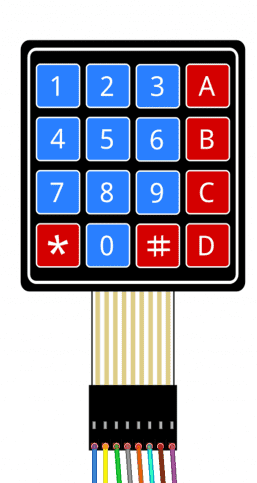
\includegraphics[width=0.4\textwidth]{images/Arduino/keypad_image.png} % Image placeholder
        \caption{Keypad}
    \end{figure}
\newpage

    \item \textbf{LCD-Screen}
    
    \textbf{Reference}: Details available at \cite{seeedstudio-lcd}
    
    \textbf{Purpose}: The LCD screen displays real-time information and system status to users, providing visual feedback about the locker system's operation.
    
    \textbf{Functionality}: The Arduino sends commands to the LCD screen to display text and graphics, enhancing user interaction and system monitoring capabilities.
    
    \begin{figure}[h]
        \centering
        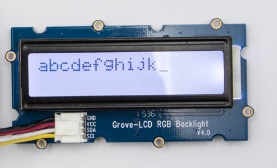
\includegraphics[width=0.5\textwidth]{images/Arduino/lcd_image.png} % Image placeholder
        \caption{LCD Screen}
    \end{figure}
\newpage
    \item \textbf{Current Sensor}
    
    \textbf{Reference}: Follow this \cite{current-sensor-tutorial} for implementation details
    
    \textbf{Purpose}: The current sensor measures electrical current flowing through a circuit, enabling monitoring of power consumption and detecting anomalies.
    
    \textbf{Functionality}: The Arduino reads analog voltage signals from the current sensor to calculate current values, which can be used for power management and safety monitoring.
    
    \begin{figure}[h]
        \centering
        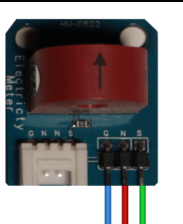
\includegraphics[width=0.4\textwidth]{images/Arduino/current_sensor_image.png} % Image placeholder
        \caption{Current Sensor}
    \end{figure}
\newpage
    \item \textbf{Door Sensor}
    
    \textbf{Reference}: Learn more about Arduino door sensors from this \cite{door-sensor-tutorial}
    
    \textbf{Purpose}: The door sensor detects the state (open or closed) of the locker door, providing security and triggering actions based on door status changes.
    
    \textbf{Functionality}: The Arduino reads digital signals from the door sensor to determine the door's position and reacts accordingly, such as activating the locking mechanism.
    
    \begin{figure}[h]
        \centering
        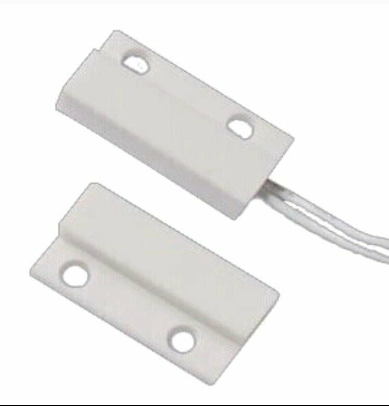
\includegraphics[width=0.5\textwidth]{images/Arduino/door_sensor_image.png} % Image placeholder
        \caption{Door Sensor}
    \end{figure}
    \newpage

    \item \textbf{Servo Motor}  
    
    \textbf{Reference}: Tutorial available at \cite{arduino-micro-servos}
    
    \textbf{Purpose}: The servo motor controls the mechanical movement of the locker's locking mechanism, enabling remote operation and automation.
    
    \textbf{Functionality}: The Arduino sends PWM signals to the servo motor to position it at specific angles, allowing precise control over the locking and unlocking of the locker.
    
    \begin{figure}[h]
        \centering
        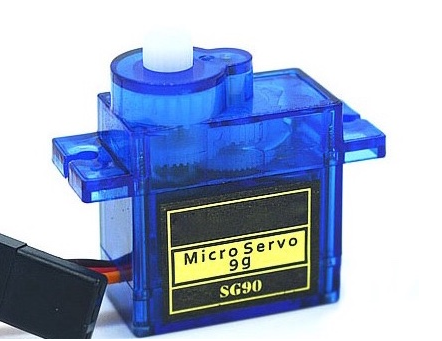
\includegraphics[width=0.5\textwidth]{images/Arduino/servo.png} % Image placeholder
        \caption{Servo Motor }
    \end{figure}
    
\end{enumerate}


\newpage
\subsubsection{Fritzing}\label{sec:ArduinoFritzing}
The image depicted in Figure \ref{fig:ardFritzing} illustrates the correct arrangement and connections of cables and components required for setting up the Arduino system as described in this guide. This visual guide, created using Fritzing software, provides a clear representation of how to wire the Arduino board with various sensors and peripherals. Referencing this diagram will ensure accurate implementation of the hardware setup outlined in the instructions.

\begin{figure}[h]
    \centering
    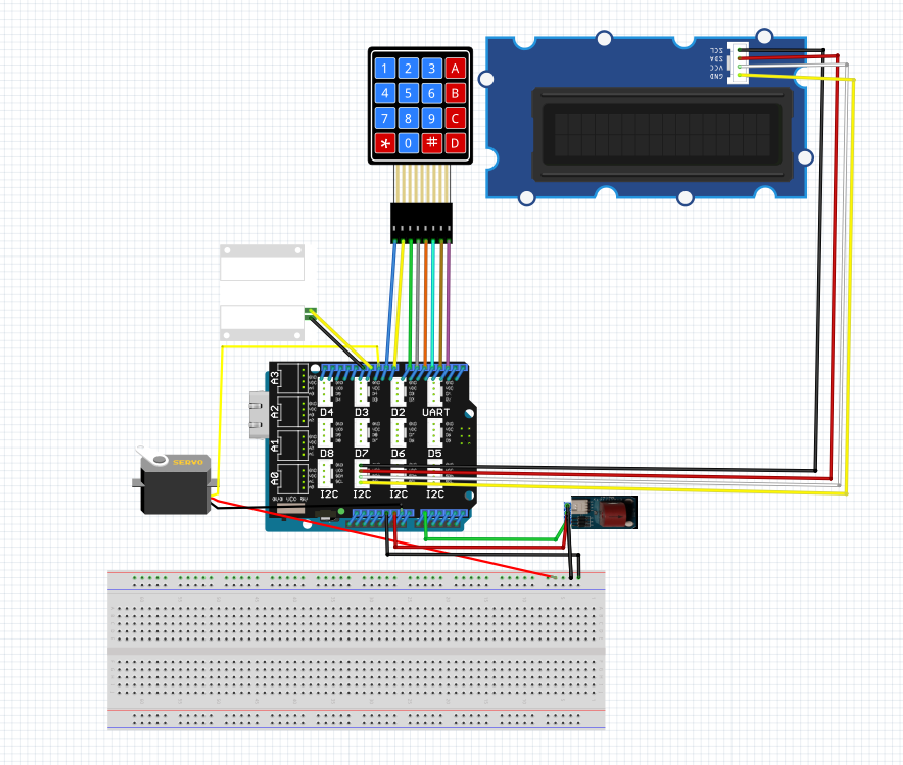
\includegraphics[width=0.8\textwidth]{images/Arduino/arduino_fritzing_curcuit.png}
    \caption{Arduino Fritzing setup}
    \label{fig:ardFritzing}
\end{figure}



\subsubsection{Areas for Improvement}

While the backend implementation of the locker system prototype adheres to common best practices, several areas require further attention and refinement before the system can be considered production-ready:

\begin{itemize}
    \item \textbf{Error Handling}: The current implementation lacks comprehensive error handling mechanisms, which are essential for gracefully managing unexpected scenarios and providing informative feedback to users. For example, enhancing error responses with appropriate status codes and error messages would improve the system's robustness.

    \item \textbf{Infrastructure}: The prototype operates in a development environment and lacks the infrastructure necessary for deployment in a production setting. Implementing scalable infrastructure components, such as load balancers, auto-scaling groups, and fault-tolerant databases, is crucial for ensuring system reliability and performance under varying workloads.

    \item \textbf{Validation}: While basic input validation is incorporated into the API endpoints, there is room for strengthening validation logic to enforce data integrity and prevent malicious inputs. Implementing robust validation mechanisms, such as input sanitization and parameter validation, would enhance the security and reliability of the system.

    \item \textbf{Security}: Security measures, including authentication, authorization, and data encryption, are fundamental requirements for safeguarding sensitive information and protecting the system against security threats. Implementing authentication mechanisms, role-based access control (RBAC), and encryption protocols would mitigate security risks and enhance the system's trustworthiness.
\end{itemize}

Addressing these areas of improvement would contribute to the development of a robust, secure, and scalable backend system for the locker application.

\section{Testing}
{\tiny Written by: Jingya Zhao}\\

\subsection{Why we test with Postman}

Here’s why using Postman to test APIs created by FastAPI is beneficial:

\begin{enumerate}
    \item \textbf{Ease of Use:} Postman provides a user-friendly interface that simplifies the process of testing APIs. With its intuitive design and features like history collections and environment, we can quickly create, organize, and execute API tests without the need for complex setups and configurations.

    \item \textbf{Real-time Feedback and Collaboration:} During the development phase, using Postman allows developers to test APIs in real-time, enabling them to identify any issues or errors promptly. For instance, when encountering an unexpected response status code of 403 (Forbidden), Postman allows us to easily share the request details with other team members. We can collaborate to rectify the issues and update the test accordingly.

    \item \textbf{Automated Testing:} We can use Postman CLI to automate collection runs on continuous integration and deployment (CI/CD) pipelines. After running the commands in the local terminal, the Postman CLI generates a link. Following the link, team members can check the detailed results.
\end{enumerate}

\subsection{How we test}

In the testing process for various functionalities of the FastAPI Inventory Management System, we adopt a systemic approach for sending HTTP requests with different methods (e.g., GET, POST, PUT, DELETE), headers, body content (in JSON format), and parameters. The testing methodology involves the following steps:

\begin{enumerate}
    \item \textbf{Request Configuration:} We configure Postman to send HTTP requests to the corresponding endpoints for each functionality being tested. We primarily utilized the GET method to retrieve data from the API endpoints related to bookings, categories, devices, users, and pins. This includes setting up appropriate headers, request bodies, and query parameters as necessary.

    \item \textbf{Test Execution:} Upon sending each request, Postman interacts with the server and awaits the response. Once the response is received, Postman triggers a series of predefined tests.

    \item \textbf{Test Result Analysis:} Postman automatically evaluates the response against the predefined tests and generates detailed test reports. We analyze these reports to identify any failed tests or errors encountered during the testing process.

    \item \textbf{Iterative Testing:} Based on the test results and feedback, we iterate on the testing process, updating test scripts, and re-executing tests as necessary to ensure comprehensive testing and validate the functionality’s correctness.
\end{enumerate}

\subsection{What we test}

The entities and their corresponding test areas include:

\begin{itemize}
    \item \textbf{Bookings:} We tested the ability to retrieve existing bookings from the system. Tests include scenarios where bookings are filtered by specific criteria using parameters such as date, user ID, and locker ID.

    \item \textbf{Categories:} Testing focused on ensuring the proper retrieval of available locker categories. Tests verify that categories are returned with their corresponding properties, such as category name and ID.

    \item \textbf{Devices:} Tests aimed to ensure proper retrieval of device information. Tests include essential details such as owner, purchase status, and device-specific information.

    \item \textbf{Users:} Tests targeted at user management functionalities. Tests verify the email address, name, role (user or admin), and ID.

    \item \textbf{Pins:} Generate Pin Functionality in detail. In the testing of the Generate Pin functionality, we focus on evaluating various aspects to ensure the correctness and reliability of the PIN generation process:
    \begin{lstlisting}[language=Java]
    // Test for HTTP status code
pm.test("Status code is 200", function () {
    pm.response.to.have.status(200);
});

// Test that the response contains a "pin" property
pm.test("Response contains a 'pin' property", function () {
    const jsonData = pm.response.json();
    pm.expect(jsonData).to.have.property("pin"); // Check for "pin" property
});

// Test that the "pin" property is an integer
pm.test("'pin' is an integer", function () {
    const jsonData = pm.response.json();
    pm.expect(jsonData.pin).to.be.a("number"); // Ensure "pin" is a number
});

// Test that the "pin" is between 1000 and 9999
pm.test("The 'pin' is a four-digit number between 1000 and 9999 and the generated 'pin' is unique", function () {
    const jsonData = pm.response.json();
    const pin = jsonData.pin;
    pm.expect(pin).to.be.within(1000, 9999); // Check if "pin" is within the four-digit range
});
\end{lstlisting}

    \begin{itemize}
        \item \textbf{HTTP Status Code Test:} We verify that the server responds with a status code of 200, indicating that the request was successful and the PIN generation endpoint is accessible.

        \item \textbf{Presence of “pin” Property Test:} We confirm that the response body contains a "pin" property, which is essential for identifying and retrieving the generated PIN.

        \item \textbf{Data Type of “pin” Property Test:} It's critical to ensure the value associated with the "pin" property is an integer. This guarantees compatibility with further processing steps within the system and adheres to the expected data format.

        \item \textbf{Validity of Generated PIN Test:} We rigorously validate that the generated PIN adheres to the predefined criteria. The PIN should be a four-digit number, falling within the range of 1000 to 9999.
    \end{itemize}
\end{itemize}

If the Postman test execution for the Generate Pin functionality resulted in all four tests passing successfully.
\begin{figure}[h]
    \centering
    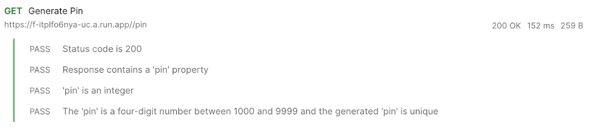
\includegraphics[width=0.8\textwidth]{images/testing1}
    \caption{Generate Pin Functionality Test results}
    \label{fig:testresults-postman}
\end{figure}
This confirms that the API endpoints behaves as intended when generating pins.

\subsection{Evaluation of test results (Automate runs via Postman CLI)}
\begin{figure}[h]
    \centering
    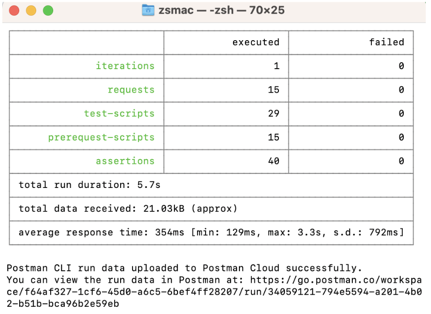
\includegraphics[width=0.8\textwidth]{images/testing2}
    \caption{Test results of Inventory Management System}
    \label{fig:testresults-postman-all}
\end{figure}
We utilise Postman’s command-line interface (CLI) to execute an automated test for our Inventory Management System. The result comprised 29 test scripts designed to verify various functionalities. As show in the picture above, the test run executed all scripts successfully, and the corresponding assertions (verification checks) passed, confirming that the system behaves as intended.
\section{Reflection and Lessons Learned}
{\tiny Written by: Sven Lepper}\\

\subsection{Successes and Effective Practices}

Reflecting on the international project to develop a locker system for universities, several valuable lessons were learned throughout the course of the project. These reflections include both the successes achieved and areas for improvement, providing insights that would guide future projects.

Overall, the project concluded with a very satisfactory outcome for us, despite the challenges posed by the tight deadline. Key factors contributing to the success of the project include:

\begin{itemize}
    \item \textbf{Effective Communication}: Maintaining open and regular communication channels proved to be essential. Through platforms such as WhatsApp and Discord, along with bi-weekly meetings, team members remained well-informed about project progress and tasks.

    \item \textbf{Positive Team Dynamics}: The cohesive spirit within the team fostered a supportive environment where members easily assisted each other. This collaborative ethos not only enhanced productivity but also facilitated mutual learning and skill development.

    \item \textbf{Utilization of Kanban Board}: Adopting a Kanban board for task organization proved to be important in visualizing workflow and tracking individual and collective progress. The transparency afforded by this tool promoted accountability and facilitated efficient task allocation.

    \item \textbf{Adaptability to Remote Work}: Despite a preference for face-to-face collaboration, the team demonstrated adaptability in transitioning to online work modes when necessary. Effective utilization of online collaboration tools enabled seamless remote teamwork.

    \item \textbf{Skill Integration through Pair Programming}: Pair programming is a collaborative development technique where two programmers work together at one workstation. One programmer, known as the "driver," writes the code, while the other, the "navigator," reviews each line as it's typed. This approach encourages constant communication, instant feedback, and shared problem-solving.

    Pair programming was the right tool for our team for several reasons. Firstly, it facilitated knowledge sharing among team members with different expertise levels. Pairing individuals allowed for the transfer of skills and knowledge in real-time, fostering a supportive environment where team members could learn from each other's experiences.

    Moreover, pair programming promoted a deeper understanding of the codebase and project requirements. The constant dialogue between the driver and navigator ensured that code was thoroughly reviewed as it was written, reducing the likelihood of errors and enhancing overall code quality. Additionally, pairing individuals with varying skill levels encouraged less experienced team members to contribute actively while receiving guidance and mentorship from more experienced team members.
\end{itemize}

\subsection{Areas for Improvement and Lessons Learned}

While the project yielded very good results, several areas were identified for improvement, along with valuable lessons learned for future projects:

\begin{itemize}
    \item \textbf{Investment in Quality Components}: An incident involving the malfunction of inexpensive Arduino components underscored the importance of investing in quality hardware. In future projects, buying higher-quality components would mitigate risks of hardware failures and enhance system reliability.

    \item \textbf{Consideration of Hosting Platforms}: Initially opting for Amazon Web Services (AWS) for hosting, the project encountered unexpected costs associated with certain AWS components. Subsequently transitioning to Google Cloud required additional effort but provided valuable exposure to alternative cloud platforms.

    \item \textbf{Consolidation of API Documentation}: We generated API documentation in two separate documents, this led to discrepancies and minor bugs. Consolidating all API documentation into a single source of truth would streamline development processes and ensure consistency across the project.

    \item \textbf{Early Testing Implementation}: We realized that initiating the testing phase earlier in the development cycle would have allowed us to identify and address bugs faster. In future projects, starting testing sooner will be a priority to reduce the time spent on debugging later in the process.
\end{itemize}

In conclusion, the international project to develop a locker system for universities provided invaluable learning experiences and insights. While celebrating the successes achieved, it is important to acknowledge areas for improvement and incorporate lessons learned into future projects.
\section{Next steps / Outlook}

This chapter presents the next steps of our project and explores possibilities 
for enhancement with additional time and resources. 
We will outline specific options and solutions to optimize and advance project outcomes. 
Through this exploration, we aim to maximize the full potential of our project 
for maximum impact and success.

\subsection{Expanding from One Locker Prototype to Locker Systems}

Currently, our system features a single locker prototype designed to demonstrate the functionality and implementation of our technology. This prototype serves as a proof of concept for showcasing our capabilities.

Moving forward, our objective is to scale our system by implementing a comprehensive locker system with customizable configurations to meet diverse needs. For example:

\begin{itemize}
    \item \textbf{Thinner Lockers for Laptops}: We plan to introduce lockers with wider compartments suitable for securely storing laptops and larger electronic devices.
    \item \textbf{Smaller Lockers for Phones and Small Items}: Additionally, we aim to offer compact lockers designed specifically for storing mobile phones, wallets, keys, and other smaller items.
    \item \textbf{Variable Compartment Sizes}: Our locker system will feature adjustable compartment sizes to accommodate various items, providing flexibility for different storage requirements.
\end{itemize}

This transition from a single prototype to a versatile locker system infrastructure represents a significant advancement in our capabilities. It enables us to cater to a wide range of applications, including secure storage solutions tailored to specific customer needs and use cases.


\subsection{Real-time Charging Level Monitoring}
The current approach involves utilizing an Arduino Current Power Sensor to measure the
current amperage flowing into the device, 
enabling determination of the charging status and current amperage. 
This method provides basic charging information but lacks insight into the battery's state of charge.

To enhance this system, our objective is to implement a more sophisticated feature that enables 
real-time monitoring of the device's charging percentage. This enhancement aims to facilitate smart and 
sustainable charging practices to mitigate premature battery degradation.


\subsection{Implementation of QR Codes for Streamlined Inventory Management}
Currently, the inventory management system relies on manual entry through an administrative interface,
 where item parameters must be manually inputted to add items to the system. 
 Searching for specific items within the database requires querying by ID, name, or other attributes.

Our proposed approach involves transitioning to a QR code-based system, where each item is assigned
 a unique QR code identifier. 
 This implementation aims to simplify inventory management by enabling rapid item identification 
 through QR code scanning, streamlining the process for administrators to locate and manage items
 within the system.

\subsection{Scheduled Maintenance Protocol}
As our system continues to grow and evolve, particularly with the increasing complexity of our inventory management,
we recognize the critical importance of ensuring reliability and performance. 
To achieve this, we are dedicated to establishing a structured and scheduled maintenance protocol. 
This protocol will enable us to proactively manage maintenance activities, optimize asset performance,
and minimize unplanned downtime, specifically targeting our inventory items. By implementing this approach,
we aim to enhance overall system reliability, support scalability,
and ensure the continuous functionality and efficiency of our inventory management processes as we expand.


\subsection{Automated Reservation System}



\section{Summary Ifdi}
To be done...

\section{Append}
Appendix



\bibliographystyle{ieeetr}
\bibliography{references}

\end{document}
